\documentclass[12pt,openany,twoside,a4paper]{book}
\usepackage[utf8]{inputenc}
\usepackage{graphicx}
\usepackage[left=2.90cm,right=2.30cm,top=2.90cm,bottom=2.30cm]{geometry}
\usepackage{hyperref}
\usepackage{arabtex}
\usepackage{utf8}
\usepackage[T1]{fontenc}
\usepackage{helvet}
\usepackage[table, xcdraw]{xcolor}
\usepackage{pagecolor}
\usepackage{afterpage}
\usepackage{float}
\usepackage{array}
\usepackage[acronym,toc,section]{glossaries}
\usepackage[english]{babel}
% TODO: use style=ieee but it brokes encoding
\usepackage[backend=biber,bibencoding=utf8]{biblatex}
\usepackage[toc,page]{appendix}
\usepackage{fancyhdr}
\usepackage{lmodern}
\usepackage{listings}
\usepackage{listings-golang}
\usepackage{enumitem}
\usepackage{multirow}
\setcounter{tocdepth}{4}
\setcounter{secnumdepth}{4}


\addbibresource{references.bib}

\newcommand{\gpProject}{C4IAN}
\newcommand{\gpYear}{2021}
\newcommand{\gpDate}{July 24, \gpYear}
\newcommand{\gpSupervisor}{Dr. Ahmed Hamdy}
\newcommand{\gpSupervisorEmail}{ahamdy@eng.cu.edu.eg}
\newcommand{\gpSupervisorMobile}{+2 01012697605}
\newcommand{\gpStudentFirst}{Abdulrahman Khalid Hassan}
\newcommand{\gpStudentFirstEmail}{abdulrahman.elshafei98@gmail.com}
\newcommand{\gpStudentFirstMobile}{+2 01011315175}
\newcommand{\gpStudentSecond}{Ahmed Mahmoud AbdEl-Monaem}
\newcommand{\gpStudentSecondEmail}{ahmed.afifi.cufe@gmail.com}
\newcommand{\gpStudentSecondMobile}{+2 01003242713}
\newcommand{\gpStudentThird}{Mahmoud Othman Adas}
\newcommand{\gpStudentThirdEmail}{mahmoud.othman.adas@gmail.com}
\newcommand{\gpStudentThirdMobile}{+2 01019426003}
\newcommand{\gpStudentFourth}{Yosry Mohammad Yosry}
\newcommand{\gpStudentFourthEmail}{yosrym93@gmail.com}
\newcommand{\gpStudentFourthMobile}{+2 01149392716}
\definecolor{gpCoverBGColor}{HTML}{FFFFFF}
\definecolor{gpCoverTextColor}{HTML}{000000}

\renewcommand*{\contentsname}{Table of Contents}
\renewcommand{\familydefault}{\sfdefault}
\newcommand\thefont{\expandafter\string\the\font}

\pagestyle{fancy}
\fancyhf{}
\cfoot{\thepage}
\fancyhead[RO]{\gpProject{} | \gpYear{}}
\fancyhead[LE]{\gpYear{} | \gpProject{}}
\fancyhead[RE,LO]{}

% list of abbreviations won't show if you don't declare and use one or more acronyms
% for more info https://www.overleaf.com/learn/latex/Glossaries#Acronyms
\makeglossaries

\newacronym{cmd}{CMD}{Command Center Client}
\newacronym{zhls}{ZHLS}{Zone Hierarchical Link state Routing}
\newacronym{odmrp}{ODMRP}{On Demand Multicast Routing Protocol}
\newacronym{vrb}{VRB}{Variable-Radius Broadcasting}
\newacronym{ui}{UI}{User Interace}
\newacronym{guis}{GUIs}{Graphical User Interfaces}
\newacronym{gui}{GUI}{Graphical User Interface}
\newacronym{ip}{IP}{Internet Protocol}
\newacronym{manets}{MANETs}{Mobile Ad-hoc Networks}
\newacronym{manet}{MANET}{Mobile Ad-hoc Network}
\newacronym{caian}{C4IAN}{Command, Control, Communications, Computing \& Intelligence using Ad-hoc Networks}
\newacronym{rnd}{R\&D}{Research and Development}
\newacronym{voip}{VoIP}{Voice Over IP}
\newacronym{poc}{PoC}{Push-to-Tablk over Cellular}
\newacronym{dmr}{DMR}{Digital Mobile Radio}
\newacronym{dsdv}{DSDV}{Destination Sequenced Distance Vector}
\newacronym{olsr}{OLSR}{Optimized Link State Routing Protocol}
\newacronym{fsr}{FSR}{Fisheye State Routing}
\newacronym{aodv}{AODV}{Ad Hoc On-Demand Distance Vector Routing
Protocol}
\newacronym{dsr}{DSR}{Dynamic Source Routing}
\newacronym{zrp}{ZRP}{Zone Routing Protocol}
\newacronym{hw}{HW}{Hardware}
\newacronym{zid}{ZID}{Zone IDentification Protocol}
\newacronym{arp}{ARP}{Address Resolution Protocol}
\newacronym{sarp}{SARP}{Secure Address Resolution Protocol}
\newacronym{mac}{MAC}{Media Access Control}
\newacronym{sse}{SSE}{Server-Side Events}
\newacronym{hal}{HAL}{Hardware Abstraction Layer}
\newacronym{api}{API}{Application Programming Interface}
\newacronym{rest}{REST}{Representational State Transfer}
\newacronym{rfc}{RFC}{Reference for Comments}
\newacronym{ebpf}{eBPF}{Extended Berkeley Packet Filter}
\newacronym{hls}{HLS}{Http Live Streaming}
\newacronym{Capex}{CAPEX}{Capital Expenses}
\newacronym{Opex}{OPEX}{Operational Expenses}
\newacronym{utils}{utils}{utilities}


% golang code listing preferences
\newcommand{\setGolang}{\lstset{%
    frame=single,
    basicstyle=\footnotesize,
    keywordstyle=\color{red},
    numbers=left,
    numbersep=5pt,
    showstringspaces=false, 
    stringstyle=\color{blue},
    tabsize=4,
    language=Golang,
    escapechar=@,
    captionpos=b
}}
\renewcommand{\lstlistingname}{Snippet}

% General Guidelines
%     • The document is intended to be a template for the graduation project report in the department of Computer Engineering, Cairo University
%     •  After reading this page, you have to remove it from the report
%     • Red texts should be removed and replaced by similar ones, related to your project
%     • The color of the cover page should be green
%     • Throughout your text, use the font type, font size, and spacing, as in this template. In general, Arial font should be used. Chapter headings should be of size 24. Sections should be of size 18, and regular text should be of size 12. Your text should be justified on both left and right sides.  
%     • The reference list should be written using a font size of 10. Ensure that the references are written correctly and all fields are included. References should be ordered according to their appearance in the text “[1], [2], [3] … etc”
%     • The table of content is a tentative one. You could add more sections as required. However, the mentioned sections should be included in your report
%     • For the appendices, add any appendix you see necessary. Remove any appendix that is not applicable to your project. However, the feasibility study and user guide should be included 
%     • Ensure that the report is clear and self-contained, such that any future interested reader could completely understand your project “to the extent of building another one similar to yours”
%     • Use figures as much as possible to clarify and enrich your discussion. You have to draw all figures yourself. Ensure that the figures are clear and their size is suitable. 
%     • Any figure caption should be inserted below the figure. Figures within any chapter should be numbered starting from 1. For example, the first figure of chapter 2 should be “Figure 2.1”. Similarly, the fourth figure of chapter 3 should be “Figure 3.4”
%     • Any table caption should be inserted above the table. Tables within any chapter should be numbered starting from 1. For example, the first table of chapter 4 should be “Table 4.1”. Similarly, the seventh table of chapter 5 should be “Table 5.7”
%     • Copy and paste from any other source is not allowed by any shape. Even for the background knowledge, you have to use your own wording.
%     • The complete report should be submitted 48 hours before the final project demonstration day. Ensure that you would meet this deadline to avoid any late penalty

\begin{document}
\setcode{utf8}

\pagenumbering{roman}
\pagecolor{gpCoverBGColor}\afterpage{\nopagecolor}
\thispagestyle{empty}
{\color{gpCoverTextColor}
\begin{figure}

\includegraphics[width=1.09in]{images/cu-logo.png}\\
{\color{gpCoverTextColor} 
Cairo University\\
Faculty of Engineering\\
Department of Computer Engineering
}
\vspace{30pt}
\end{figure}

\begin{center}
    \vspace{10pt}
    {\fontsize{32}{50} \selectfont \textbf{\gpProject{}}}
    \vspace{15pt}
    
    \begin{figure}[H]
    \centering
    
\includegraphics[width=0.5\linewidth]{images/logo.png}
    \label{fig:logo}
    \end{figure}

    \vspace{10pt}
    \textbf{A Graduation Project Report Submitted}
    \vspace{3pt}\\
    to
    \vspace{3pt}\\
    \textbf{Faculty of Engineering, Cairo University} 
    \vspace{3pt}\\
    \textbf{in Partial Fulfillment of the requirements of the degree}
    \vspace{3pt}\\
    of
    \vspace{3pt}\\
    \textbf{Bachelor of Science in Computer Engineering}
    \vspace{10pt}
    
    \vspace{15pt}
    {\Large \textbf{Presented by}}\\
    \begin{center}
    \begin{tabular}{ l c r }
     \textbf{\gpStudentFirst} & \hspace{50pt} & \textbf{\gpStudentSecond} \\
     \textbf{\gpStudentThird} & \hspace{50pt} & \textbf{\gpStudentFourth}
    \end{tabular}
    \end{center}
    
    \vspace{8pt}
    {\Large \textbf{Supervised by}}\\
    \vspace{5pt}
    \textbf{\gpSupervisor}
    
    \vspace{15pt}
    \textbf{\gpDate{}}
    
    \vspace{10pt}
    All rights reserved. This report may not be reproduced in whole or in part, by photocopying or other means, without the permission of the authors/department.    
\end{center}
\newpage
}

\section*{Abstract}
\label{sec:abstract}
\addcontentsline{toc}{section}{\nameref{sec:abstract}}

% The abstract should clearly and briefly describe the project objective(s) and outcome(s). In details, the abstract should include, but not limited to, all of the following:
%     \begin{itemize}
%         \item The problem(s) which is(are) addressed in the project
%         \item The objective(s) of the project
%         \item The approach that is followed to solve the problem
%         \item The output(s) of the project
%         \item Testing/development tools and summary of testing results
%         \item The sponsor(s), if any
%     \end{itemize}

\quad \acrfull{manets} is an ever-growing research field due to their numerous practical applications. \acrshort{manets} provide means for infrastructure-less communications, they are utilized by tactical teams, military, emergency and rescue teams, drone swarms, and many others. \\

\acrshort{caian} (\acrlong{caian}) is a scalable communications solution for tactical teams. It builds a \acrshort{manet} on-the-go between command centers and units, allowing them to communicate effectively and securely while moving freely, without the need for any infrastructure. \\

Our system can be run on handheld tactical devices, robots, drones, or any other Linux-based platform. It features both a platform-independent network layer which routes data through dynamically changing and scalable topologies, and applications for tactical teams’ units and command centers to communicate through. \\

\acrshort{caian}'s router implements \acrfull{zhls} routing for uni-casting, \acrfull{odmrp} for multi-casting, and a unique \acrfull{vrb} that is based on \acrshort{zhls}. We also introduced some improvements to \acrshort{zhls} and \acrshort{odmrp} to optimize their implementation.

\newpage

\begin{arabtext}
{\huge
المُلَخَّص
}\vspace{20pt}
الشبكات التلقائية المتحركة تلقي رواجاً كبيرة كمجال للبحث العلمي حيث أن لها عدداً كبيراً من التطبيقات العملية. الشبكات التلقائية المتحركة توفر طريقة للتواصل بدون بنية تحتية, و لها مستخدمون عديدون, مثل الفرق التكتيكية, و الجيوش, وفرق الطوارئ و الإنقاذ, و الروبوتات, و غيرهم.
\vspace{\baselineskip}
كيان هو نظام تواصل معتمد للفرق التكتيكية. كيان يقوم ببناء شبكة تلقائية عند الحاجة بين مراكز التحكم و الوحدات, ممكناً إياهم من التواصل بشكل سريع و آمن أثناء التحرك بحرية, بدون الحاجة إلي بنية تحتية.
\vspace{\baselineskip}
نظام كيان يمكن تشغليه علي أجهزة التواصل المحمولة الخاصة بالفرق التكتيكية, أو علي روبوتات, أو علي أي جهاز يدعم نظام تشغيل لينكس. النظام قادر علي تحديد مسار البيانات و توجيهها داخل الشبكات كبيرة الحجم المتغيرة بسرعة, بالإضافة إلي برنامجين لوحدات الفرق التكتيكية و مراكز القيادة.
\vspace{\baselineskip}
موجه البيانات في كيان يستخدم بروتوكول توجيه 
هرمي مبني على المناطق للبيانات الموجهة لوجهة واحدة, و بروتوكل توجيه متعدد عند الحاجة للبيانات الموجهة لعدة جهات, و بروتوكول نشر المعلومات لقطر معين لتوجيه البيانات الموجهة للجميع. لقد قمنا أيضاً بإضافة بعض التحسينات علي هذه البروتوكولات.

\end{arabtext}
\newpage

\section*{Acknowledgment}
\addcontentsline{toc}{section}{Acknowledgment}
\quad Our gratitude to those who helped us cannot be put in words. First, we would like to express our appreciation and thankfulness to our supervisor, \textbf{Dr. Ahmed Hamdy}, for his utmost care and support for us during our work. His guidance and mentorship have been critical to our success. \\

We would also like to thank our family, friends and colleagues, who have always been there to support us and push us forward. We are defined by the people who surround us, and those people made us who we are today.
\newpage

\tableofcontents
\addcontentsline{toc}{section}{\contentsname}

\listoffigures
\addcontentsline{toc}{section}{List of Figures}

\listoftables
\addcontentsline{toc}{section}{List of Tables}

\clearpage

\printglossary[type=\acronymtype,title=List of Abbreviations]

\clearpage

\section*{Contacts}
\label{sec:contacts}
\addcontentsline{toc}{section}{\nameref{sec:contacts}}

\subsubsection*{\centering Team Members}
\rowcolors{2}{gray!25}{white}
{
\centering
\begin{tabular}{|l | l | l|}
\rowcolor{gray!50}
    \hline
    Name & Email & Phone Number\\\hline\hline
    \gpStudentFirst & \gpStudentFirstEmail & \gpStudentFirstMobile\\\hline
    \gpStudentSecond & \gpStudentSecondEmail & \gpStudentSecondMobile\\\hline
    \gpStudentThird & \gpStudentThirdEmail & \gpStudentThirdMobile\\\hline
    \gpStudentFourth & \gpStudentFourthEmail & \gpStudentFourthMobile\\\hline
\end{tabular}
}

\subsubsection*{\centering Supervisor}
\rowcolors{2}{gray!25}{white}
\begin{center}
\begin{tabular}{|l | l | l|}
\rowcolor{gray!50}
    \hline
    Name & Email & Phone Number\\\hline\hline
    \gpSupervisor & \gpSupervisorEmail & \gpSupervisorMobile\\\hline
\end{tabular}
\end{center}

\clearpage
\vspace*{\fill}
\begin{center}
\begin{minipage}{.45\textwidth}
This page is intentionally left blank
\end{minipage}
\end{center}
\vfill % equivalent to \vspace{\fill}
\clearpage
\chapter{Introduction}
\pagenumbering{arabic}
% This chapter is to introduce your project, justify the need for it and explain the steps you follow to achieve it. The main outcomes from the project should be clearly stated. The organization of the document should finally be given

% In this space, before the first section, write a general introduction to the project

An ad-hoc network is a decentralized network that does not rely on pre-existing infrastructure. There are no dedicated routers or access points. Instead, hosts (user devices) act as both a user and a router in the network. When a message is sent, it gets forwarded between different nodes in the network until it reaches its destination.\cite{wu2004ad} \cite{ramanathan2002brief} \\

\acrfull{manets} are a type of wireless ad-hoc networks where the devices can move freely. This increases the versatility of the network, and extends its use cases to more practical applications. Nonetheless, the routing problem becomes much more complex as the topology of the network is changing dynamically. Links between devices are frequently broken, and devices need to be up-to-date with the most recent version of the topology to be able to communicate. Furthermore, as the network size increases, keeping track of such a dynamic topology becomes even harder.\cite{mohapatra2004ad} \\

Naturally, \acrshort{manets} have always been an active area of research due to the complexity of the routing problem. Different approaches to the routing problem are being researched continuously, with very few practical implementations. \\

\acrshort{caian} (\acrlong{caian}) is a scalable communications solution for tactical teams. It builds a \acrshort{manet} on-the-go between command centers and units, allowing them to communicate effectively and securely while moving freely, without the need for any infrastructure.

\section{Motivation and Justification}
Tactical teams, such as emergency and rescue teams, police officers, and military battalions, require a robust communications solution. They cannot rely on infrastructure-based communications (such as cellular networks) for multiple reasons:
\begin{itemize}[itemsep=1pt, topsep=5pt]
    \item They can be damaged during an emergency or a catastrophe.
    \item They are unavailable in remote areas.
    \item They can be easily targeted by enemies.
    \item Commercial ones may not be secure enough.
\end{itemize}
Hence, \acrshort{manets} are usually the obvious means of communications for such tactical teams. \acrshort{caian} aims to provide a software \acrshort{manet}-based communications solution for tactical teams, that can be deployed on any Linux platform.

\section{Project Objectives and Problem Definition}
We aim to build a scalable software system that provides reliable communications between devices that are moving freely, without any infrastructure. The core of such a system is routing. Our core objective is to develop a scalable \acrshort{manet} routing solution that will be the basis of a concrete communications system. \\

\acrshort{manet} routing is an open-ended research problem. There are no established protocols that work for all use cases. \acrshort{caian} implements unicast, multicast, and broadcast routing. For each type of routing, there are many protocols in the research literature, with very few implementations. We surveyed many protocols, selected and tuned adequate ones, and morphed the results of theoretical research into concrete practical implementations.

\section{Project Outcomes}
The outcome of the project is two-fold. The core part is a Linux-based network layer that implements unicast, multicast, and broadcast routing. The customer-facing part is an application that utilizes this network layer to provide communications to command centers and units in a tactical team.

\section{Document Organization}
In this chapter, we provided an introduction to \acrshort{manets} and to our communications system for tactical teams, \acrshort{caian}. The rest of the document is organized as follows:
\begin{itemize}[itemsep=1pt, topsep=5pt]
    \item In chapter 2 we discuss the potential market for our product, and the competition we may face.
    \item In chapter 3 we review different approaches to unicast and multicast routing in \acrshort{manets}, and lay the necessary background to understand the routing problem. 
    \item In chapter 4 we explain how our system works. We dive deep into the architecture of \acrshort{caian} and discover what every module contributes.
    \item In chapter 5 we explain how we tested different aspects of our system, and how it compares to related work.
    \item In chapter 6 we conclude the document by describing the challenges we faced, the lessons that we learned, and what the future may look like for \acrshort{caian}.
\end{itemize}

Afterwards, the appendices outline the development platforms and tools that we used, different use cases of \acrshort{caian}, the user guide, code documentation, and a comprehensive feasibility study.

\chapter{Market Feasibility Study}
Achieving scalable and reliable communications in areas that lack network infrastructure is a difficult problem, especially in critical situations such as the battlefield or during emergencies. It is also needed for collecting real time data and analyze it to have a competitive advantage in the battleground.
\\
\acrfull{manets} can be formed on-the-go, without any infrastructure. They promise more flexibility and reliability than manual radio broadcasting.
\\

\section{Targeted Customers}
Our initial market will be the tactical teams by providing tactical system and its products for defense industry, rescue teams and police we will provide in yearly subscription for using our products, training and support. As our team gets sophisticated enough, our target customer base will widen, and we will build another solution to fit a normal customer using the same router module. We will build a communication/streaming/gaming service and target customers who do not have internet infrastructure in their area, by providing additional servers in their areas which will act as routers and have significant caches of movies and web data.

\section{Market Survey}
\subsection{Bittium}
% https://www.bittium.com/index.php?id=2167&locate=PRM%2F2020%2F3729781
Bittium [\ref{}] specializes in the development of reliable, secure communications and connectivity solutions with experience over 35 years in advanced radio communication technologies. Bittium provides innovative products and services, customized solutions based on its product platforms and \acrfull{rnd} services. Complementing its communications and connectivity solutions, Bittium offers proven information security solutions for mobile devices and portable computers. Bittium also provides healthcare technology products and services for biosignal measuring in the areas of cardiology, neurology, rehabilitation, occupational health and sports medicine. Net sales in 2020 were EUR 78.4 million and operating profit was EUR 2.1 million.
\\
\\
Bittium offers communication options, which are critical in combat. Bittium TAC WIN, the company's primary competing product, is a high-performance wireless network solution that enables fast and flexible link, point-to-multipoint, and \acrshort{manet} (Mobile Ad Hoc Network) connections.
\\
The system enables improved connection to current wired and wireless IP infrastructures and legacy systems, as well as broadband IP data transmission for mobility troops in all areas of the battlefield. 
\\
\\
The Estonian Defense Forces requested a tactical communication network based on the Bittium TAC WIN system.
\\
The TAC WIN system will be used to modernize IP data transmission, improve the performance of the tactical data transmission, and diversify the wireless and cable connections of the Estonian Land Forces' system entity.
\\
The Bittium Tough \acrfull{voip} product family's products will be used to upgrade the Land Forces' IP voice service, and when combined with the Bittium TAC WIN system, it forms a software solution that seamlessly integrates the tactical network and its voice services for leading troops in the most demanding situations.
\\
\\
On July 1, 2021, Bittium has received another purchased order from the Finnish Defense Forces for the development of a new software version for the software defined radio based Bittium Tactical Wireless IP Network system.
\\
The purchase order is worth roughly 2.3 million EUR (excl. VAT), with extra purchases with a maximum value of 0.5 million EUR (excl. VAT) are included in the procurement decision.
The development work will be completed by the end of the first half of 2022.
\subsection{Hytera}
% https://www.hytera.com/
Hytera [\ref{}] is a Chinese manufacturer of radio transceivers and radio systems. Hytera's sales and revenue in 2020 is 6.06 Billion dollars [\ref{}].
% https://www.wsj.com/market-data/quotes/CN/002583/financials
\\
\\
Hytera provides two types of products \acrfull{dmr} and \acrfull{poc} systems and applications.
The main competitor product is Hytera HALO Dispatch which is a \acrfull{poc} radio systems that enables countrywide or single-site communications and dispatching, as well as rapid group calling that supports data, audio, and video. The three systems are capable of functioning as stand-alone networks.
\\
Hytera Halo Dispatch Software is billed annually. The first year is $999, each additional year is $599.00.

\section{Business Case and Financial Analysis }
The target product of our company is to produce the entire system from A to Z by request. The unit cost is estimated to range from 3000 to 5000 EGP, including its testing. The command center device cost is estimated to range from 8,000 to 10,000 EGP including its testing.
In this section, two aspects will be addressed:
\begin{enumerate}[itemsep=1pt, topsep=5pt]
    \item Business Case.
    \item Financial Analysis.
\end{enumerate}

\subsection{Business Case}
In the business case, we will illustrate the projected amount of product sales over the next five years, which is shown in Table \ref{tbl:business-case}, as well as how we will adjust the pricing to compete.

\begin{center}
\begin{table}[!htbp]
\centering
\begin{tabular}{|c|c|cccc}
\cline{1-2}
\rowcolor[HTML]{C0C0C0} 
\cellcolor[HTML]{C0C0C0}{\color[HTML]{343434} \textbf{Years}}                                  & \cellcolor[HTML]{C0C0C0}{\color[HTML]{343434} \textbf{Year 1}}                         & {\color[HTML]{343434} \textbf{Year 2}}                                                                                             & {\color[HTML]{343434} \textbf{Year 3}}                                                                                             & {\color[HTML]{343434} \textbf{Year 4}}                                                                                             & {\color[HTML]{343434} \textbf{Year 5}}                                                                                             \\ \hline
\rowcolor[HTML]{FFFFFF} 
\textbf{CMD Ordered}                                                                           & \textbf{1,000}                                                                         & \multicolumn{1}{c|}{\cellcolor[HTML]{FFFFFF}\textbf{2,000}}                                                                        & \multicolumn{1}{c|}{\cellcolor[HTML]{FFFFFF}\textbf{3,000}}                                                                        & \multicolumn{1}{c|}{\cellcolor[HTML]{FFFFFF}\textbf{5,000}}                                                                        & \multicolumn{1}{c|}{\cellcolor[HTML]{FFFFFF}\textbf{10,000}}                                                                       \\ \hline
\rowcolor[HTML]{FFFFFF} 
\cellcolor[HTML]{FFFFFF}\textbf{Units Ordered}                                                 & \cellcolor[HTML]{FFFFFF}\textbf{10,000}                                                & \multicolumn{1}{c|}{\cellcolor[HTML]{FFFFFF}\textbf{15,000}}                                                                       & \multicolumn{1}{c|}{\cellcolor[HTML]{FFFFFF}\textbf{20,000}}                                                                       & \multicolumn{1}{c|}{\cellcolor[HTML]{FFFFFF}\textbf{50,000}}                                                                       & \multicolumn{1}{c|}{\cellcolor[HTML]{FFFFFF}\textbf{80,000}}                                                                       \\ \hline
\rowcolor[HTML]{FFFFFF} 
\cellcolor[HTML]{FFFFFF}\textbf{CMD Cost}                                                      & \textbf{10,000}                                                                        & \multicolumn{1}{c|}{\cellcolor[HTML]{FFFFFF}\textbf{10,100}}                                                                       & \multicolumn{1}{c|}{\cellcolor[HTML]{FFFFFF}\textbf{10,300}}                                                                       & \multicolumn{1}{c|}{\cellcolor[HTML]{FFFFFF}\textbf{10,500}}                                                                       & \multicolumn{1}{c|}{\cellcolor[HTML]{FFFFFF}\textbf{10,550}}                                                                       \\ \hline
\rowcolor[HTML]{FFFFFF} 
\textbf{Unit Cost}                                                                             & \textbf{4,000}                                                                         & \multicolumn{1}{c|}{\cellcolor[HTML]{FFFFFF}\textbf{4,200}}                                                                        & \multicolumn{1}{c|}{\cellcolor[HTML]{FFFFFF}\textbf{4,400}}                                                                        & \multicolumn{1}{c|}{\cellcolor[HTML]{FFFFFF}\textbf{4,600}}                                                                        & \multicolumn{1}{c|}{\cellcolor[HTML]{FFFFFF}\textbf{4,650}}                                                                        \\ \hline
\rowcolor[HTML]{FFFFFF} 
\cellcolor[HTML]{FFFFFF}\textbf{\begin{tabular}[c]{@{}c@{}}Purchased \\ CMD Cost\end{tabular}} & \cellcolor[HTML]{FFFFFF}\textbf{\begin{tabular}[c]{@{}c@{}}22,000 \\ EGP\end{tabular}} & \multicolumn{1}{c|}{\cellcolor[HTML]{FFFFFF}\textbf{\begin{tabular}[c]{@{}c@{}}25,000 \\ EGP\end{tabular}}}                        & \multicolumn{1}{c|}{\cellcolor[HTML]{FFFFFF}\textbf{\begin{tabular}[c]{@{}c@{}}30,000 \\ EGP\end{tabular}}}                        & \multicolumn{1}{c|}{\cellcolor[HTML]{FFFFFF}\textbf{\begin{tabular}[c]{@{}c@{}}40,000 \\ EGP\end{tabular}}}                        & \multicolumn{1}{c|}{\cellcolor[HTML]{FFFFFF}\textbf{\begin{tabular}[c]{@{}c@{}}41,000 \\ EGP\end{tabular}}}                        \\ \hline
\rowcolor[HTML]{FFFFFF} 
\textbf{\begin{tabular}[c]{@{}c@{}}Purchased \\ Unit Cost\end{tabular}}                        & \textbf{\begin{tabular}[c]{@{}c@{}}10,000 \\ EGP\end{tabular}}                         & \multicolumn{1}{c|}{\cellcolor[HTML]{FFFFFF}\textbf{\begin{tabular}[c]{@{}c@{}}12,000 \\ EGP\end{tabular}}}                        & \multicolumn{1}{c|}{\cellcolor[HTML]{FFFFFF}\textbf{\begin{tabular}[c]{@{}c@{}}15,000 \\ EGP\end{tabular}}}                        & \multicolumn{1}{c|}{\cellcolor[HTML]{FFFFFF}\textbf{\begin{tabular}[c]{@{}c@{}}17,000 \\ EGP\end{tabular}}}                        & \multicolumn{1}{c|}{\cellcolor[HTML]{FFFFFF}\textbf{\begin{tabular}[c]{@{}c@{}}17,500 \\ EGP\end{tabular}}}                        \\ \hline
\rowcolor[HTML]{FFFFFF} 
\textbf{\begin{tabular}[c]{@{}c@{}}Profit From \\ Purchasing\end{tabular}}                     & \textbf{\begin{tabular}[c]{@{}c@{}}72M\\  EGP\end{tabular}}                     & \multicolumn{1}{c|}{\cellcolor[HTML]{FFFFFF}\textbf{\begin{tabular}[c]{@{}c@{}}146.8M \\ EGP\end{tabular}}}                        & \multicolumn{1}{c|}{\cellcolor[HTML]{FFFFFF}\textbf{\begin{tabular}[c]{@{}c@{}}271.1M\\ EGP\end{tabular}}}                         & \multicolumn{1}{c|}{\cellcolor[HTML]{FFFFFF}\textbf{\begin{tabular}[c]{@{}c@{}}767.5M\\  EGP\end{tabular}}}                        & \multicolumn{1}{c|}{\cellcolor[HTML]{FFFFFF}\textbf{\begin{tabular}[c]{@{}c@{}}1.3325B\\ EGP\end{tabular}}}                        \\ \hline
\rowcolor[HTML]{FFFFFF} 
\textbf{\begin{tabular}[c]{@{}c@{}}Profit From \\ Maintenance\end{tabular}}                    & \textbf{\begin{tabular}[c]{@{}c@{}}2M \\ EGP\end{tabular}}                             & \multicolumn{1}{c|}{\cellcolor[HTML]{FFFFFF}\textbf{\begin{tabular}[c]{@{}c@{}}4M \\ EGP\end{tabular}}}                            & \multicolumn{1}{c|}{\cellcolor[HTML]{FFFFFF}\textbf{\begin{tabular}[c]{@{}c@{}}6M\\  EGP\end{tabular}}}                            & \multicolumn{1}{c|}{\cellcolor[HTML]{FFFFFF}\textbf{\begin{tabular}[c]{@{}c@{}}10M\\ EGP\end{tabular}}}                            & \multicolumn{1}{c|}{\cellcolor[HTML]{FFFFFF}\textbf{\begin{tabular}[c]{@{}c@{}}20M\\ EGP\end{tabular}}}                            \\ \hline
\rowcolor[HTML]{FFFFC7} 
\cellcolor[HTML]{FFFFC7}{\color[HTML]{34696D} \textbf{Total Profit}}                           & {\color[HTML]{34696D} \textbf{\begin{tabular}[c]{@{}c@{}}74M\\  EGP\end{tabular}}}     & \multicolumn{1}{c|}{\cellcolor[HTML]{FFFFC7}{\color[HTML]{34696D} \textbf{\begin{tabular}[c]{@{}c@{}}150.8M\\  EGP\end{tabular}}}} & \multicolumn{1}{c|}{\cellcolor[HTML]{FFFFC7}{\color[HTML]{34696D} \textbf{\begin{tabular}[c]{@{}c@{}}277.1M\\  EGP\end{tabular}}}} & \multicolumn{1}{c|}{\cellcolor[HTML]{FFFFC7}{\color[HTML]{34696D} \textbf{\begin{tabular}[c]{@{}c@{}}777.5M\\  EGP\end{tabular}}}} & \multicolumn{1}{c|}{\cellcolor[HTML]{FFFFC7}{\color[HTML]{34696D} \textbf{\begin{tabular}[c]{@{}c@{}}1.3525B\\ EGP\end{tabular}}}} \\ \hline
\end{tabular}
\caption{Business case over 5 years}
\label{tbl:business-case}
\end{table}
\end{center}

\subsection{Financial Analysis}
Financial analysis is done based on the company's business case to predict the Capital Expenses (Capex) and the Operational Expenses (Opex).
\\
Table \ref{tbl:capex-table} displays the Capex and Table \ref{tbl:opex-table} shows the Opex.

\begin{center}
\begin{table}[!htbp]
\centering
\begin{tabular}{|c|c|}
\hline
\rowcolor[HTML]{C0C0C0} 
{\color[HTML]{343434} \textbf{Items And Supplies}}                                                                            & {\color[HTML]{343434} \textbf{Cost}}       \\ \hline
\rowcolor[HTML]{FFFFFF} 
\textbf{\begin{tabular}[c]{@{}c@{}}Offices, chairs, air conditioners, \\ security cameras, routers and switches\end{tabular}} & \textbf{90,000 EGP}                        \\ \hline
\rowcolor[HTML]{FFFFFF} 
\textbf{Developers Laptops}                                                                                                   & \textbf{10 * 15 = 150,000 EGP}             \\ \hline
\rowcolor[HTML]{FFFFFF} 
\textbf{\begin{tabular}[c]{@{}c@{}}30 units of Raspberry Pi\\  4 Model B 4 GB for testing\end{tabular}}                        & \textbf{1,720.00 * 30 = 51,600 EGP}         \\ \hline
\rowcolor[HTML]{FFFFFF} 
\textbf{\begin{tabular}[c]{@{}c@{}}30 units of RC Waterproof 2.4Ghz \\ All Terrain Off-Road Amphibious Car\end{tabular}}      & \textbf{600 * 30 = 18,000 EGP}              \\ \hline
\rowcolor[HTML]{FFFFC7} 
{\color[HTML]{34696D} \textbf{Total Capex}}                                                                                   & {\color[HTML]{34696D} \textbf{409,600 EGP}} \\ \hline
\end{tabular}
\caption{Capex Table}
\label{tbl:capex-table}
\end{table}

\begin{table}[!htbp]
\centering
\begin{tabular}{|c|c|}
\hline
\rowcolor[HTML]{C0C0C0} 
{\color[HTML]{343434} \textbf{Items And Supplies}}                                                & {\color[HTML]{343434} \textbf{Cost per Month}} \\ \hline
\rowcolor[HTML]{FFFFFF} 
\textbf{Employees' salaries}                                                                      & \textbf{150,000 EGP}                           \\ \hline
\rowcolor[HTML]{FFFFFF} 
\textbf{Office Rent}                                                                              & \textbf{4,000 EGP}                              \\ \hline
\rowcolor[HTML]{FFFFFF} 
\multicolumn{1}{|l|}{\cellcolor[HTML]{FFFFFF}\textbf{Training customers and testing fields Rent}} & \textbf{12,000 EGP}                            \\ \hline
\rowcolor[HTML]{FFFFFF} 
\textbf{Office maintenance}                                                                       & \textbf{2,000 EGP}                              \\ \hline
\rowcolor[HTML]{FFFFFF} 
\textbf{Servers maintenance}                                                                      & \textbf{3,000 EGP}                              \\ \hline
\rowcolor[HTML]{FFFFFF} 
\textbf{\begin{tabular}[c]{@{}c@{}}Bills (electricity, water, gas, \\ etc.)\end{tabular}}         & \textbf{2,000 EGP}                              \\ \hline
\rowcolor[HTML]{FFFFC7} 
{\color[HTML]{34696D} \textbf{Total Opex}}                                                        & {\color[HTML]{34696D} \textbf{173,000 EGP}}     \\ \hline
\end{tabular}
\caption{Opex Table}
\label{tbl:opex-table}
\end{table}



\begin{table}[!htbp]
\centering
\resizebox{18cm}{!}{%
\begin{tabular}{|c|c|c|c|c|c|c|c|c|c|c|c|c|}
\hline
\rowcolor[HTML]{C0C0C0} 
\multicolumn{13}{|c|}{\cellcolor[HTML]{C0C0C0}{\color[HTML]{343434} \textbf{Money Going Out}}}                                                                                                                                                                                                                                                                                                                                                                                                                                                                                                                                                                                                                                                                                                                                                                                                                                                                                                                                                           \\ \hline
\rowcolor[HTML]{C0C0C0} 
\cellcolor[HTML]{C0C0C0}{\color[HTML]{343434} \textbf{Month}}                                       & \cellcolor[HTML]{C0C0C0}{\color[HTML]{343434} \textbf{1}} & {\color[HTML]{343434} \textbf{2}}        & {\color[HTML]{343434} \textbf{3}}        & {\color[HTML]{343434} \textbf{4}}        & {\color[HTML]{343434} \textbf{5}}                                                        & {\color[HTML]{343434} \textbf{6}}                                                        & {\color[HTML]{343434} \textbf{7}}                                                        & {\color[HTML]{343434} \textbf{8}}                                                        & {\color[HTML]{343434} \textbf{9}}                                                        & {\color[HTML]{343434} \textbf{10}}                                                       & {\color[HTML]{343434} \textbf{11}}                                                       & {\color[HTML]{343434} \textbf{12}}                                                       \\ \hline
\rowcolor[HTML]{C0C0C0} 
\multicolumn{13}{|c|}{\cellcolor[HTML]{C0C0C0}{\color[HTML]{343434} \textbf{Capex}}}                                                                                                                                                                                                                                                                                                                                                                                                                                                                                                                                                                                                                                                                                                                                                                                                                                                                                                                                                                     \\ \hline
\rowcolor[HTML]{FFFFFF} 
\cellcolor[HTML]{FFFFFF}\textbf{Office}                                                             & \cellcolor[HTML]{FFFFFF}\textbf{7,500}                    & \textbf{7,500}                           & \textbf{7,500}                           & \textbf{7,500}                           & \textbf{7,500}                                                                           & \textbf{7,500}                                                                           & \textbf{7,500}                                                                           & \textbf{7,500}                                                                           & \textbf{7,500}                                                                           & \textbf{7,500}                                                                           & \textbf{7,500}                                                                           & \textbf{7,500}                                                                           \\ \hline
\rowcolor[HTML]{FFFFFF} 
\cellcolor[HTML]{FFFFFF}\textbf{Laptops}                                                            & \cellcolor[HTML]{FFFFFF}\textbf{12,500}                   & \textbf{12,500}                          & \textbf{12,500}                          & \textbf{12,500}                          & \textbf{12,500}                                                                          & \textbf{12,500}                                                                          & \textbf{12,500}                                                                          & \textbf{12,500}                                                                          & \textbf{12,500}                                                                          & \textbf{12,500}                                                                          & \textbf{12,500}                                                                          & \textbf{12,500}                                                                          \\ \hline
\rowcolor[HTML]{FFFFFF} 
\cellcolor[HTML]{FFFFFF}\textbf{\begin{tabular}[c]{@{}c@{}}30 Unit \\ Raspberry \\ Pi\end{tabular}} & \cellcolor[HTML]{FFFFFF}\textbf{4,300}                    & \textbf{4,300}                           & \textbf{4,300}                           & \textbf{4,300}                           & \textbf{4,300}                                                                           & \textbf{4,300}                                                                           & \textbf{4,300}                                                                           & \textbf{4,300}                                                                           & \textbf{4,300}                                                                           & \textbf{4,300}                                                                           & \textbf{4,300}                                                                           & \textbf{4,300}                                                                           \\ \hline
\rowcolor[HTML]{FFFFFF} 
\cellcolor[HTML]{FFFFFF}\textbf{30 Unit Car}                                                        & \cellcolor[HTML]{FFFFFF}\textbf{1,500}                    & \textbf{1,500}                           & \textbf{1,500}                           & \textbf{1,500}                           & \textbf{1,500}                                                                           & \textbf{1,500}                                                                           & \textbf{1,500}                                                                           & \textbf{1,500}                                                                           & \textbf{1,500}                                                                           & \textbf{1,500}                                                                           & \textbf{1,500}                                                                           & \textbf{1,500}                                                                           \\ \hline
\rowcolor[HTML]{C0C0C0} 
\multicolumn{13}{|c|}{\cellcolor[HTML]{C0C0C0}{\color[HTML]{343434} \textbf{Opex}}}                                                                                                                                                                                                                                                                                                                                                                                                                                                                                                                                                                                                                                                                                                                                                                                                                                                                                                                                                                      \\ \hline
\rowcolor[HTML]{FFFFFF} 
\textbf{Salaries}                                                                                   & \cellcolor[HTML]{FFFFFF}\textbf{150,000}                  & \textbf{150,000}                         & \textbf{150,000}                         & \textbf{150,000}                         & \textbf{150,000}                                                                         & \textbf{150,000}                                                                         & \textbf{150,000}                                                                         & \textbf{150,000}                                                                         & \textbf{150,000}                                                                         & \textbf{150,000}                                                                         & \textbf{150,000}                                                                         & \textbf{150,000}                                                                         \\ \hline
\rowcolor[HTML]{FFFFFF} 
\cellcolor[HTML]{FFFFFF}\textbf{\begin{tabular}[c]{@{}c@{}}Office\\ Rent\end{tabular}}              & \textbf{4,000}                                            & \textbf{4,000}                           & \textbf{4,000}                           & \textbf{4,000}                           & \textbf{4,000}                                                                           & \textbf{4,000}                                                                           & \textbf{4,000}                                                                           & \textbf{4,000}                                                                           & \textbf{4,000}                                                                           & \textbf{4,000}                                                                           & \textbf{4,000}                                                                           & \textbf{4,000}                                                                           \\ \hline
\rowcolor[HTML]{FFFFFF} 
\textbf{\begin{tabular}[c]{@{}c@{}}Fields\\ Rent\end{tabular}}                                      & \textbf{12,000}                                           & \textbf{12,000}                          & \textbf{12,000}                          & \textbf{12,000}                          & \textbf{12,000}                                                                          & \textbf{12,000}                                                                          & \textbf{12,000}                                                                          & \textbf{12,000}                                                                          & \textbf{12,000}                                                                          & \textbf{12,000}                                                                          & \textbf{12,000}                                                                          & \textbf{12,000}                                                                          \\ \hline
\rowcolor[HTML]{FFFFFF} 
\textbf{\begin{tabular}[c]{@{}c@{}}Office\\ Maintenance\end{tabular}}                               & \textbf{2,000}                                            & \textbf{2,000}                           & \textbf{2,000}                           & \textbf{2,000}                           & \textbf{2,000}                                                                           & \textbf{2,000}                                                                           & \textbf{2,000}                                                                           & \textbf{2,000}                                                                           & \textbf{2,000}                                                                           & \textbf{2,000}                                                                           & \textbf{2,000}                                                                           & \textbf{2,000}                                                                           \\ \hline
\rowcolor[HTML]{FFFFFF} 
\cellcolor[HTML]{FFFFFF}\textbf{\begin{tabular}[c]{@{}c@{}}Servers\\ Maintenance\end{tabular}}      & \cellcolor[HTML]{FFFFFF}\textbf{3,000}                    & \textbf{3,000}                           & \textbf{3,000}                           & \textbf{3,000}                           & \textbf{3,000}                                                                           & \textbf{3,000}                                                                           & \textbf{3,000}                                                                           & \textbf{3,000}                                                                           & \textbf{3,000}                                                                           & \textbf{3,000}                                                                           & \textbf{3,000}                                                                           & \textbf{3,000}                                                                           \\ \hline
\rowcolor[HTML]{FFFFFF} 
\cellcolor[HTML]{FFFFFF}\textbf{Bills}                                                              & \textbf{2,000}                                            & \textbf{2,000}                           & \textbf{2,000}                           & \textbf{2,000}                           & \textbf{2,000}                                                                           & \textbf{2,000}                                                                           & \textbf{2,000}                                                                           & \textbf{2,000}                                                                           & \textbf{2,000}                                                                           & \textbf{2,000}                                                                           & \cellcolor[HTML]{FFFFFF}\textbf{2,000}                                                   & \textbf{2,000}                                                                           \\ \hline
\rowcolor[HTML]{FFFFC7} 
{\color[HTML]{329A9D} \textbf{Total Out}}                                                           & {\color[HTML]{329A9D} \textbf{198,800}}                   & {\color[HTML]{329A9D} \textbf{198,800}}  & {\color[HTML]{329A9D} \textbf{198,800}}  & {\color[HTML]{329A9D} \textbf{198,800}}  & {\color[HTML]{329A9D} \textbf{198,800}}                                                  & {\color[HTML]{329A9D} \textbf{198,800}}                                                  & {\color[HTML]{329A9D} \textbf{198,800}}                                                  & {\color[HTML]{329A9D} \textbf{198,800}}                                                  & {\color[HTML]{329A9D} \textbf{198,800}}                                                  & {\color[HTML]{329A9D} \textbf{198,800}}                                                  & {\color[HTML]{329A9D} \textbf{198,800}}                                                  & {\color[HTML]{329A9D} \textbf{198,800}}                                                  \\ \hline
\rowcolor[HTML]{C0C0C0} 
\multicolumn{13}{|c|}{\cellcolor[HTML]{C0C0C0}{\color[HTML]{343434} \textbf{Money Going In}}}                                                                                                                                                                                                                                                                                                                                                                                                                                                                                                                                                                                                                                                                                                                                                                                                                                                                                                                                                            \\ \hline
\rowcolor[HTML]{FFFFFF} 
\textbf{\begin{tabular}[c]{@{}c@{}}Total CMD\\ \& Unit \\ Purchased\\ Profits\end{tabular}}         & \textbf{0}                                                & \textbf{0}                               & \textbf{0}                               & \textbf{0}                               & \textbf{925,000}                                                                         & \textbf{925,000}                                                                         & \textbf{925,000}                                                                         & \textbf{925,000}                                                                         & \textbf{925,000}                                                                         & \textbf{925,000}                                                                         & \textbf{925,000}                                                                         & \textbf{925,000}                                                                         \\ \hline
\rowcolor[HTML]{FFFFFF} 
\cellcolor[HTML]{FFFFFF}\textbf{Maintainance}                                                       & \cellcolor[HTML]{FFFFFF}\textbf{0}                        & \textbf{0}                               & \textbf{0}                               & \textbf{0}                               & \textbf{500,00}                                                                          & \textbf{500,00}                                                                          & \textbf{500,00}                                                                          & \textbf{500,00}                                                                          & \textbf{500,00}                                                                          & \textbf{500,00}                                                                          & \textbf{500,00}                                                                          & \textbf{500,00}                                                                          \\ \hline
\rowcolor[HTML]{FFFFC7} 
{\color[HTML]{329A9D} \textbf{Total In}}                                                            & {\color[HTML]{329A9D} \textbf{0}}                         & {\color[HTML]{329A9D} \textbf{0}}        & {\color[HTML]{329A9D} \textbf{0}}        & {\color[HTML]{329A9D} \textbf{0}}        & {\color[HTML]{329A9D} \textbf{\begin{tabular}[c]{@{}c@{}}1.425\\ Million\end{tabular}}}  & {\color[HTML]{329A9D} \textbf{\begin{tabular}[c]{@{}c@{}}1.425\\ Million\end{tabular}}}  & {\color[HTML]{329A9D} \textbf{\begin{tabular}[c]{@{}c@{}}1.425\\ Million\end{tabular}}}  & {\color[HTML]{329A9D} \textbf{\begin{tabular}[c]{@{}c@{}}1.425\\ Million\end{tabular}}}  & {\color[HTML]{329A9D} \textbf{\begin{tabular}[c]{@{}c@{}}1.425\\ Million\end{tabular}}}  & {\color[HTML]{329A9D} \textbf{\begin{tabular}[c]{@{}c@{}}1.425\\ Million\end{tabular}}}  & {\color[HTML]{329A9D} \textbf{\begin{tabular}[c]{@{}c@{}}1.425\\ Million\end{tabular}}}  & {\color[HTML]{329A9D} \textbf{\begin{tabular}[c]{@{}c@{}}1.425\\ Million\end{tabular}}}  \\ \hline
\rowcolor[HTML]{FFFFC7} 
{\color[HTML]{329A9D} \textbf{Profit}}                                                              & {\color[HTML]{329A9D} \textbf{-198,800}}                  & {\color[HTML]{329A9D} \textbf{-198,800}} & {\color[HTML]{329A9D} \textbf{-198,800}} & {\color[HTML]{329A9D} \textbf{-198,800}} & {\color[HTML]{329A9D} \textbf{\begin{tabular}[c]{@{}c@{}}1.2262\\ Million\end{tabular}}} & {\color[HTML]{329A9D} \textbf{\begin{tabular}[c]{@{}c@{}}1.2262\\ Million\end{tabular}}} & {\color[HTML]{329A9D} \textbf{\begin{tabular}[c]{@{}c@{}}1.2262\\ Million\end{tabular}}} & {\color[HTML]{329A9D} \textbf{\begin{tabular}[c]{@{}c@{}}1.2262\\ Million\end{tabular}}} & {\color[HTML]{329A9D} \textbf{\begin{tabular}[c]{@{}c@{}}1.2262\\ Million\end{tabular}}} & {\color[HTML]{329A9D} \textbf{\begin{tabular}[c]{@{}c@{}}1.2262\\ Million\end{tabular}}} & {\color[HTML]{329A9D} \textbf{\begin{tabular}[c]{@{}c@{}}1.2262\\ Million\end{tabular}}} & {\color[HTML]{329A9D} \textbf{\begin{tabular}[c]{@{}c@{}}1.2262\\ Million\end{tabular}}} \\ \hline
\rowcolor[HTML]{FFFFC7} 
{\color[HTML]{329A9D} \textbf{Net Profit}}                                                          & {\color[HTML]{329A9D} \textbf{-198,800}}                  & {\color[HTML]{329A9D} \textbf{-397,600}} & {\color[HTML]{329A9D} \textbf{-596,400}} & {\color[HTML]{329A9D} \textbf{-795,200}} & {\color[HTML]{329A9D} \textbf{431,000}}                                                  & {\color[HTML]{329A9D} \textbf{\begin{tabular}[c]{@{}c@{}}1.6572\\ Million\end{tabular}}} & {\color[HTML]{329A9D} \textbf{\begin{tabular}[c]{@{}c@{}}2.8834\\ Million\end{tabular}}} & {\color[HTML]{329A9D} \textbf{\begin{tabular}[c]{@{}c@{}}4.1096\\ Million\end{tabular}}} & {\color[HTML]{329A9D} \textbf{\begin{tabular}[c]{@{}c@{}}5.3358\\ Million\end{tabular}}} & {\color[HTML]{329A9D} \textbf{\begin{tabular}[c]{@{}c@{}}6.562\\ Million\end{tabular}}}  & {\color[HTML]{329A9D} \textbf{\begin{tabular}[c]{@{}c@{}}7.7882\\ Million\end{tabular}}} & {\color[HTML]{329A9D} \textbf{\begin{tabular}[c]{@{}c@{}}9.0144\\ Million\end{tabular}}} \\ \hline
\end{tabular}
}
\caption{Cache Flow Table in (EGP)}
\label{tbl:cache-flow-table}

\end{table}
\end{center}

As can be seen in the Cash  Flow  Table \ref{tbl:cache-flow-table}, it is expected that we do not sell any units or command center devices for the first four months. These four months are dedicated for testing and training troops. We should break even by the beginning of May With a net profit value of \textbf{431,000 EGP}. The main profit contribution comes from the purchase, not the support.
\\
This means that depending only on maintenance is not a good strategy, and that we should always keep our customers happy with reasonable prices and excellent services.
\\
Our product is the only one of its kind in the Middle East. Moreover, our product is so much cheaper than our competitors outside the Middle East. Hytera Halo Dispatch Software mentioned in the previous section is an example. It costs \$999 per unit per year. They also adopt a different business model and they depend more on the annual subscription.
\\
In our case, we build the system unit or CMD and sell it one time with a maintenance subscription, which is so much cheaper than selling annual subscription used by other companies.

\chapter{Literature Survey}
\label{ch:literature-survey}

\quad This section will present an overview of the literature on routing protocols in \acrshort{manet}. An ad-hoc routing protocol is a convention or standard that regulates how nodes choose which method to route data between computing devices in a mobile ad-hoc network. According to the desired destination, ad-hoc network routing techniques are split into three types: unicast routing for a single destination, multicast routing for a group of destinations, and lastly broadcast routing for all targets in the network.

A comprehensive discussion of unicast routing protocols in \acrshort{manet}, particularly \acrshort{zhls} (our implemented approach), is given in sections 3.1, 3.2, and 3.3. In sections 3.3, 3.4, and 3.5, we will discuss multicast routing protocols, particularly \acrshort{odmrp} (our implemented approach).

\section{Unicast Routing in \acrshort{manets}}
\qquad The research interest in mobile ad-hoc networking grew rapidly in the 1990s. Because of the network's lack of infrastructure and dynamic nature, new networking methods must be adopted in order to ensure efficient end-to-end communication. This, combined with the numerous applications of these networks in various circumstances such as the battlefield and disaster recovery, has resulted in \acrshort{manets} routing being studied by a variety of organizations and institutes. The majority of \acrshort{manet} applications rely on unicast connectivity. The source mobile node transmits data packets to the destination in unicast mode. The destination address in the data packet is used by the dispatch node to search it up in the routing table when forwarding data packets\cite{unicast1}. \\

It's not easy to forward packets in a \acrshort{manet} with restricted resources (such as bandwidth restrictions, concealed terminals, and low battery power). To do this, a number of protocols have been developed. To decrease packet loss, communication overheads, and enhance data delivery ratio, various \acrshort{manet} unicast routing protocols have concentrated on attaining stability and dependability. Other unicast routing protocols have placed a premium on scalability to be capable of dealing with huge networks with minimum  computations. Other protocols placed an emphasis on data transmission speed and the ability to meet real-time constraints. To attain those objectives, many techniques have been developed. A comparative study of these Unicast routing techniques will be proposed in the next section.

\section{Comparative study of Unicasting}
The fundamental goal of ad-hoc routing protocols is to efficiently transmit data packets between nodes without relying on preset topologies or centralized management. Any unicast routing protocol must have the following characteristics: 
\begin{itemize}[itemsep=1pt, topsep=5pt]
    \item It should be assumed that routes are unidirectional.
    \item It should consider data security.
    \item It must be energy-and-power-efficient.
    \item It should be distributed in such a way as to enhance its dependability.
\end{itemize}  

Based on the previous properties, unicast routing techniques in \acrshort{manets} can be divided into three classes based on the time it takes for nodes to obtain a route to a destination. Those classes are reactive, proactive, and hybrid.

\subsection{Proactive routing protocols}
Proactive routing protocols, also known as table-driven routing protocols, require each node to maintain one or more tables containing up-to-date and consistent routing information for all other nodes in the network. these protocols learn the network's global topology by sharing information across network nodes. The nodes send out update messages every time the topology changes, and the knowledge about this change is disseminated across the network. Using this information, the shortest path can be computed from each source to any destination, but on the other side a lot of bandwidth is consumed\cite{unicast2}. In the following sections, some proactive routing protocols will be discussed.

\subsubsection{\acrfull{dsdv}}
The \acrfull{dsdv} is an extension of the well-known wired routing Distance Vector protocol. \acrshort{dsdv} addresses the primary problem associated with distance vector routing protocol in wired networks by utilizing destination sequence numbers, namely count-to-infinity. old routes and new routes are distinguished using sequence numbers originated at the destination, enabling the routing protocol to avoid route loops. multiple routes with the same sequence number are distinguished using the shortest route metric.\cite{abd2009performance}


\subsubsection{\acrfull{olsr}}
\acrfull{olsr} is an also extension and optimized variant of the well-known pure link-state routing protocol. It uses a multipoint relaying technique to efficiently transmit link-state packets. As the traditional link-state routing protocol, by sending link-state messages on a regular basis, each node keeps track of the network's topology. The optimization is mostly accomplished in two ways. First, during each route update, the size of the control packets for a specific node is reduced heavily by exchanging just a subset of links with the node's neighbors who are its multipoint relay selectors, rather than all links in the network. Each packet may be read and processed by any node not in the set, but it cannot be retransmitted. Second, it reduces control traffic flooding by employing just chosen nodes, known as multipoint relays, to distribute information in the network. Each node broadcasts a list of its one-hop neighbors to select these multipoint relaying nodes. A subset of these one-hop neighbors are chosen  from the list of nodes in the hello messages that covers all of its two-hop neighbors. Node A in Figure \ref{fig:multipoint relays} can choose MPR nodes from nodes B, C, K, and N. Because these nodes cover all nodes that are two hops apart.\cite{clausen2003optimized} \cite{clausen2003rfc3626}

\begin{figure}[!htb]
    \centering
    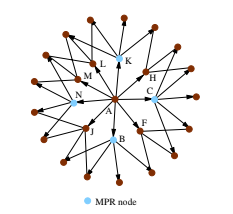
\includegraphics[scale=1]{images/olsr-mpr.png}
    \caption{Multipoint relays}
    \label{fig:multipoint relays}
\end{figure}

\subsubsection{\acrfull{fsr}}
\acrfull{fsr} is another optimized variant of the link-state routing protocol. It effectively reduces the amount of information and time it takes to keep network topology up to date. Link state updates are created and flooded across the network anytime a topology change is detected in the traditional link state routing method. However, in \acrshort{fsr}, nodes only communicate link status information on a periodic basis. By updating network information for local nodes at a higher frequency than for faraway nodes beyond the fisheye scope, \acrshort{fsr} lowers the size of update messages. As a result, \acrshort{fsr} is more scalable for huge networks. Figure \ref{fig:fsr} illustrate the \acrshort{fsr} hierarchical scopes.\cite{sathish2011comparative}

\begin{figure}[!htb]
    \centering
    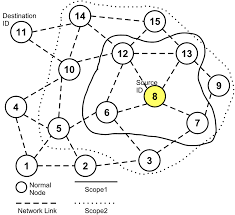
\includegraphics[scale=1]{images/fsr.png}
    \caption{Fisheye hierarchical scopes}
    \label{fig:fsr}
\end{figure}

\subsection{Reactive routing protocols}
On demand routing systems are also known as reactive protocols. By preserving route information for active routes, such protocol decreased the overheads of proactive protocol. It means that routing information is only necessary and stored when a node wishes to transmit a data packet to a specific destination. From the previous description, we can deduce that the main advantage for the reactive routing protocols over proactive routing protocol is to reduce the bandwidth waste. When route discovery is less frequent than data transmission, reactive routing systems function effectively\cite{unicast3}. Route discovery is generally accomplished by flooding the network with route request packets. When route discovery is less frequent than data transmission, reactive routing systems function effectively. 

\subsubsection{\acrfull{aodv}} 
With low control overhead and route acquisition delay, \acrfull{aodv} creates efficient routes on demand.
\acrshort{aodv} is essentially a hybrid of \acrfull{dsr} and \acrshort{dsdv} algorithms, using \acrshort{dsr}'s fundamental on-demand route discovery and maintenance mechanism as well as \acrshort{dsdv}'s usage of hop-by-hop routing sequence numbers to ensure loop-free routing. The source broadcasts a route request packet to determine a path from source to destination. The neighbors then broadcast the packet to their neighbors until it reaches an intermediary node with up-to-date route information about the destination or the destination itself. Because the route reply packet takes the same path as the route request packet, \acrshort{aodv} only needs symmetric connections. The nodes along the path insert the forward route into their tables as the route reply packet travels back to the source. Figure \ref{fig:aodv} illustrate the \acrshort{aodv} route discovery process. \cite{chakeres2004aodv} \cite{royer2000implementation}

\begin{figure}[!htb]
    \centering
    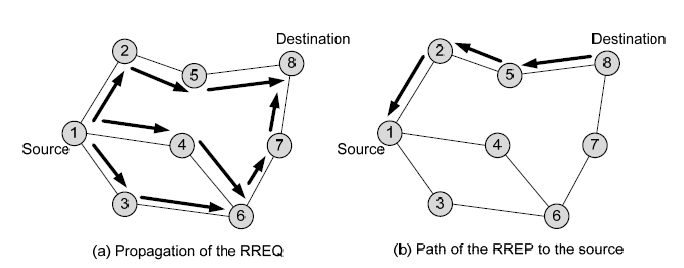
\includegraphics[scale=0.6]{images/aodv.png}
    \caption{\acrshort{aodv} route discovery}
    \label{fig:aodv}
\end{figure}

\subsubsection{\acrfull{dsr}}
\acrfull{dsr} offers a lot of advantages over routing protocols like \acrshort{aodv}, and it may perform better on small networks. \acrshort{dsr} has the benefit of allowing nodes to keep numerous routes in their route cache, allowing the node that wants to send a packet to some destination to check its route cache for a valid route before beginning route discovery, and if one is discovered, route discovery is not required. However, \acrshort{dsr} has a serious problem when dealing with huge networks, as its packets must carry the entire address (all hops in the path from source to destination). This indicates that this protocol will be ineffective on huge networks since the amount of overhead carried in each packet will grow as the network diameter grows, and it will consume a huge amount of bandwidth. Figure \ref{fig:dsr} illustrate how \acrshort{dsr} packets look like. \cite{usop2009performance} \cite{johnson2001dsr}

\begin{figure}[!htb]
    \centering
    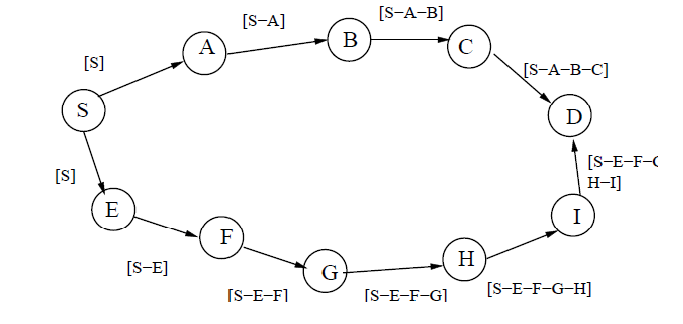
\includegraphics[scale=0.5]{images/dsr.png}
    \caption{\acrshort{dsr} packets}
    \label{fig:dsr}
\end{figure}

\subsection{Hybrid Routing Protocols}
Hybrid routing protocols are a new breed of protocol that is proactive as well as reactive. These protocols are intended to improve scalability by allowing nodes in proximity to collaborate to build a backbone that reduces route-finding overheads. The majority of this is accomplished by proactively maintaining routes to nearby nodes and finding routes to distant nodes using a route discovery strategy. The majority of hybrid protocols suggested to date are zone-based\cite{hybrid}, which implies that each node sees the network as a series of zones. In the next subsection, the \acrshort{zrp} routing protocol will be discussed, while in the next section the \acrshort{zhls} routing protocol will be discussed as our implemented approach.

\subsubsection{\acrfull{zrp}}
The nodes in \acrshort{zrp} each have a routing zone, which specifies a range (in hops) within which each node must maintain proactive network communication. As a result, routes are immediately available for nodes within the routing zone. Routes are determined on-demand for nodes outside the routing zone, and any on-demand routing protocol can be used to find a route to the needed destination. When compared to pure proactive protocols, this protocol has considerably reduced the amount of communication overhead. By allowing routes to be identified faster, it has also decreased the latency associated with pure reactive protocols like \acrshort{dsr}. This is because, in order to identify a route to a node outside the routing zone, the routing simply needs to go to a node on the required destination's borders (routing zone's edge). The drawback of \acrshort{zrp} is that it can operate as a pure proactive protocol for high values of routing zone, but as a reactive protocol for small values. \cite{beijar2002zone}

\subsubsection{\acrfull{zhls}}
\acrfull{zhls} split the whole network into zones that do not overlap. Each node in such a non-overlapping zone has a unique zone ID computed by GPS, and remember that each node in the whole network has a unique IP. The network's hierarchical structure (topology) is divided into two levels: node level topology and zone level topology, as shown in Figure \ref{fig:zhls}. Intrazone and interzone routing tables are created by each node using the flooded interzone and interzone LSR packets. When a node wants to transfer data packets to a node in another zone, the source node broadcasts a zone level “destination zone discovery (DZD)” request to all neighbor zones, which need much less overhead than reactive protocols' flooding techniques. After obtaining the destination zone, the data packets may be forwarded to the needed destination zone and subsequently to the required target node using the interzone then intrazone routing tables.\cite{joa1999peer} \cite{garg2012review} \cite{bansal2011performance} \cite{kamidate2007fault}

\begin{figure}[!htb]
    \centering
    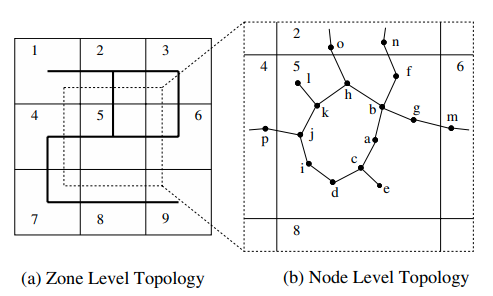
\includegraphics[scale=0.8]{images/zhls.png}
    \caption{\acrshort{zhls} network structure}
    \label{fig:zhls}
\end{figure}

\subsection{Overall Comparison of All Unicast
Routing Protocols }

Summary comparison of unicast routing protocols can be shown in Table \ref{tbl:unicast-comparison}
  
\begin{center}
\begin{table}[!htb]
\centering
\begin{tabular}{|>{\columncolor[HTML]{C0C0C0}}c |c|c|c|}
\hline
\textbf{
\begin{tabular}[c]{@{}c@{}}Routing Protocol\\ Parameter
\end{tabular}} &
  \cellcolor[HTML]{C0C0C0}\textbf{Proactive} &
  \cellcolor[HTML]{C0C0C0}\textbf{Reactive} &
  \cellcolor[HTML]{C0C0C0}\textbf{Hybrid} \\ \hline
\textbf{
\begin{tabular}[c]{@{}c@{}}Storage\\ Requirement
\end{tabular}} &
  High &
  Low &
  \begin{tabular}[c]{@{}c@{}}Depends on size\\ of each zone
  \end{tabular} \\ \hline
\textbf{\begin{tabular}[c]{@{}c@{}}Route\\ Availability\end{tabular}} &
  \begin{tabular}[c]{@{}c@{}}Always\\ available\end{tabular} &
  \begin{tabular}[c]{@{}c@{}}Computed as\\ per need\end{tabular} &
  \begin{tabular}[c]{@{}c@{}}Depends on\\ location of\\ destination\end{tabular} \\ \hline
\textbf{\begin{tabular}[c]{@{}c@{}}Periodic Route\\ Updates\end{tabular}} &
  Frequent &
  Sporadic &
  \begin{tabular}[c]{@{}c@{}}Used inside each\\ zone\end{tabular} \\ \hline
\textbf{Delay} &
  Low &
  High &
  \begin{tabular}[c]{@{}c@{}}Low for local\\ destinations and\\ high for interzone\end{tabular} \\ \hline
\textbf{Scalability} &
  100 nodes &
  \textgreater 100 nodes &
  \textgreater 1000 nodes \\ \hline
\textbf{Control Traffic} &
  High &
  Low &
  Medium \\ \hline
\textbf{\begin{tabular}[c]{@{}c@{}}Routing\\ Information\end{tabular}} &
  \begin{tabular}[c]{@{}c@{}}
  Stored in\\ table
  \end{tabular} &
  \begin{tabular}[c]{@{}c@{}}
  Does not\\ store
  \end{tabular} &
  \begin{tabular}[c]{@{}c@{}}
  Depends on\\ requirement
  \end{tabular} \\ \hline
\textbf{
\begin{tabular}[c]{@{}c@{}}
Routing\\ Philosophy
\end{tabular}} &
  Flat &
  Flat &
  Hierarchical \\ \hline
\end{tabular}
\caption{Summary Comparison of Unicast Routing Protocols}
\label{tbl:unicast-comparison}
\end{table}
\end{center}

\section{Implemented Unicast Routing: \acrshort{zhls}}
From the previous comparison, we can deduce that, in completely proactive protocols, nodes constantly attempt to maintain routes to all other nodes. This implies they monitor all topology changes in real-time. When there are a lot of nodes with a high mobility rate, this might be challenging, and it will consume a lot of bandwidth. On the other side, in completely reactive protocols, nodes only receive routing information on demand, and paths are only built when nodes have data for a specific destination. These techniques cut routing costs significantly, but their performance is variable since they are never prepared for disruptive occurrences.

We determined that a hybrid routing approach that combines aspects of both proactive and reactive routing techniques would best meet our application needs in light of these constraints. 

As stated above, Zone-Based Hierarchical Link State (\acrshort{zhls}) is one of the best hybrid routing protocols for many reasons. The management of \acrshort{zhls} nodes locations has been simplified. This is because the data transfer is not coordinated by a cluster head or a location manager. When compared to previous hybrid routing protocols, this implies there is no processing cost associated with cluster-head or Location Manager selection. This also implies that traffic bottlenecks and single points of failure may be avoided. When compared to pure reactive protocols like \acrshort{dsr} and \acrshort{aodv}, \acrshort{zhls} offers lower communication overheads. Consider the scenario when a route to a remote destination is needed (i.e., interzone routing). The source node broadcasts a zone-level location request to all other zones, resulting in much less overhead when compared to reactive protocols' flooding approach. Another advantage of \acrshort{zhls} is that the routing path may adapt to changing topologies because just the destination's node ID and zone ID are required for routing. As long as the destination does not relocate to another zone, no additional location searches are necessary.

The reasons we chose \acrshort{zhls} as a unicast routing method are summarized in the following points:

\begin{itemize}[itemsep=1pt, topsep=5pt]
    \item Simple location management as there is no cluster head or location manager node.
    \item It's ideal for tactical teams that are divided into groups and zones by nature.
    \item No traffic bottlenecks or single points of failure.
    \item Less memory requirements compared to proactive protocols.
    \item Lower control messages overhead using zone-level broadcasting compared to reactive protocols' flooding.
    \item Fewer computations when data is ready, so reduced battery usage as compared to reactive protocols.
    \item No location search is required as soon as the destination zone is known.
\end{itemize} 

There is always room for optimization. \acrshort{zhls} is one of the best unicast hybrid routing protocols but with some modifications, it can be better. The zone size is one of the most vexing aspects of any hybrid routing technology, particularly \acrshort{zhls}. The size of a zone has a significant impact on network performance. There is always a better zone size than another, depending on the application and the mobility of the nodes. So we thought, why not make the zone size a variable that the user may set depending on the application?
That was explained in details in system design section.

The second change was a technical one that affected the algorithm's implementation rather than its behavior. There will be nodes-level topology and zone-level topology, as well as intrazone and interzone forwarding tables, according to \acrshort{zhls}. Consider the scenario when a route to a remote destination is needed. the source node have to apply the shortest path algorithm on both zone-level topology and node-level topology and look at both interzone and intrazone tables depending on the destination zone. With adding one layer of abstraction to both nodes and zones, we managed to encapsulate both node IP and zone ID in one class. So now there's only one topology that contain both nodes and zones, there is also one forwarding table for both. That modifications imply fewer computations and less memory and battery consumption.

In comparison to the previous method, the third and final update significantly improves router performance and saves a significant amount of bandwidth. As previously stated, \acrshort{zhls} is a hybrid routing system, which implies it incorporates proactive routing approaches. The periodic changing of Interzone LSR control messages, which is used to convey zone information throughout the network, is one of these characteristics. The original technique required each node in each zone to flood this message, but just one node from each zone is enough because all nodes in the same zone will flood the same data. So, using some criteria, we were able to assign this work to only one node in each zone, greatly reducing control message overhead and improving system efficiency.


\section{Multicast Routing in \acrshort{manets}}
Multicast routing allows you to support group-oriented applications while using less bandwidth. Because of the growing demand for such applications, as well as the inherent characteristics of \acrshort{manets} such as lack of infrastructure and node mobility, secure multicast routing has become a critical yet difficult topic.

Multicast is an essential communication pattern that involves the sending of packets among a group of two or more hosts, and therefore is suitable for group-oriented computing. The use of multicasting in \acrshort{manets} has several benefits. For example, it can lower the cost of communication and increase the accuracy of the wireless channel, while transmitting numerous copies of the same data by exploiting the inherent broadcasting characteristics of wireless transmission. Instead of delivering data via multiple unicast connections, multicasting lowers channel capacity usage, reduces the cost of the sender and router's processing and energy, and communication latency. \cite{junhai2008research} \cite{junhai2009survey}

\subsection{Classification Of Multicast Routing Protocol}
Figure \ref{fig:mc-classification} demonstrates the dependency between the different and the main classification aspects for multicast routing protocol, including multicast topology, initialization approach, routing scheme, and maintenance approach.
\begin{figure}[!htb]
    \centering
    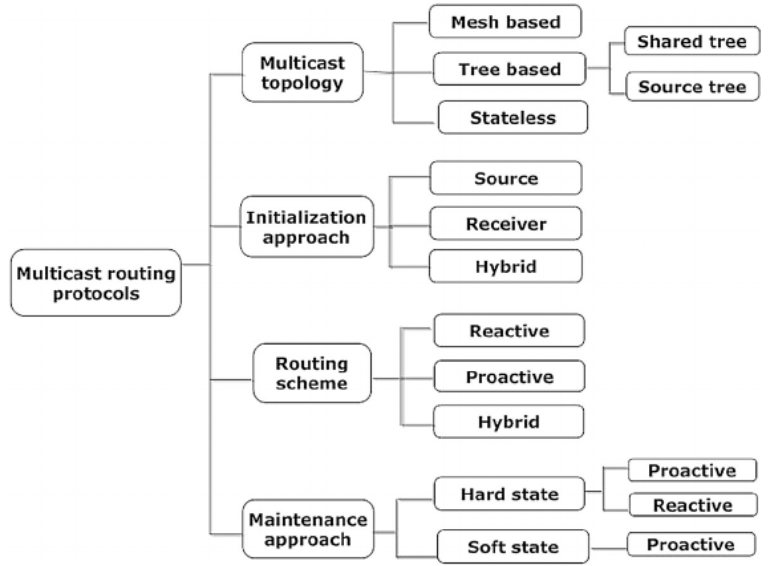
\includegraphics[scale=0.5]{images/mc-classification.png}
    \caption{classification of multicast routing protocols}
    \label{fig:mc-classification}
\end{figure}

\subsubsection{Multicast Topology}
Multicast topology has three approaches which are tree-based, mesh-based, and stateless approach. These three methods are described as follows:

\begin{enumerate}
\item Mesh-based approach

Mesh-based multicast protocols could have many routes between the same source and receiver pair. Current studies demonstrate that tree-based protocols are not always the best fit for multicast in a \acrshort{manet} when network topology changes often. In such an environment, mesh-based protocols tend to outperform tree-based approaches given the availability of different routes, which allows multicast datagram packets to be sent to the receivers even if connections fail. In this method, numerous routes are built in the whole network. These redundant routes are essential in link failure situation and give better packet delivery ratio 

\item Tree-based approach

Most systems for providing multicast in wired networks seem to be either source-tree-based or shared-tree-based. A unique route between source and receiver exists. This path and other paths are controlled by a general purpose node named core-node.

There are two main types of tree-based approach, which are described as follows:

\begin{itemize}
\item first is source-tree-based, whereby each source establishes a separated tree that includes the source node as the root node and then all receivers exist under this node.
\item second is shared-tree-based, in which one tree is created in the overall system, which contains all sources and receivers, so in this case, a core node controls the tree and behaves as a root to the tree.
\end{itemize}

\item Stateless approach

The stateless multicast approach, in which the source node explicitly specifies the list of targets in the packet header, is suggested to reduce the impact of such issues in tree-based and mesh-based approaches. Stateless multicast focuses on specific group multicast and expects the underlying routing protocol would take care of delivering the packet to appropriate destinations based on the addresses provided in the header.
\end{enumerate}

\subsubsection{Routing Initialization Approach}
Routing initialization is classified into three methods which are source-initiated, receiver-initiated, and hybrid approach. The three methods are described as follows:

\begin{enumerate}
\item Source-initiated approach

It is a method in which the multicast group creation and maintenance functions are handled by the source node. In order to start a new multicast group, the source node broadcasts a join query message all across the network, and any node wishing to join that multicast group responds by a join reply message. 

\item Receiver-initiated approach

It is a method in which the receiver node looks for a dedicated source inside the multicast group. The receiver node broadcasts a join query message across the network to enter a new multicast group, and thus the source node or core node responds by a join reply message containing the multicast group core route. 

\item Hybrid approach

The multicast group creation and maintenance functions are handled by either the source node or the receiver node in this method, which integrates specific characteristics from the source-initiated and receiver-initiated approaches. 
 
\end{enumerate}

\subsubsection{Routing Scheme}
Routing scheme is classified into three methods which are table-driven (proactive), on-demand (reactive), and hybrid approach. The three methods are described as follows:

\begin{enumerate}
\item Table-Driven Scheme (Proactive)

In a network using a proactive routing protocol, every node keeps one or more tables describing the complete network topology. These tables are frequently updated in order to keep up-to-date routing information of each node to any other node. To keep routing information up-to-date, topological information has to be transmitted between the nodes on a frequent basis, resulting in relatively significant overhead on the network. But on the other hand, routes will always be accessible on request. 

\item On-demand scheme (Reactive)

It attempts to build up routes on-demand, if a node wishes to start communication with another node to which it has no path, the routing protocol would seek to construct such a path. Reactive multicast routing protocol offers higher scalability than proactive multicast routing protocol. Unfortunately, while using reactive multicast routing protocol, source nodes may suffer from extra delay for path finding before they may send data packets. 

\item Hybrid scheme

It integrates the proactive and reactive methods in one strategy, in order to overcome the limits of both protocols and enhance their benefits. An example of a hybrid approach is zone routing protocol, which stores routing tables for a local zone, and creates routes on demand for targets outside this local neighborhood. It restricts the range of the local zone by describing a maximum hop number for the local zone. 
\end{enumerate}

\subsubsection{Multicast Maintenance Approaches}
Multicast maintenance is classified into two methods which are soft-state, and hard-state approaches. The two methods are described as follows:

\begin{enumerate}
\item Soft-state approach

This is a method in which broken link repair operation is started regularly by flooding the network with continuous control packets to seek alternative paths between source and destination. This method has the benefit of reliability and improved packet delivery ratios, but it creates considerable overhead over the network as it repeatedly floods the network with control packets. 

\item Hard-state approach

This is a method in which broken links maintenance procedure is created by two kinds, including reactive and proactive. In reactive methods, broken link recovery procedure is started only when a connection breaks. The second kind is proactive strategy, in which routes are reconfigured before a connection breaks, and this may be accomplished by using local prediction methods based on GPS or signal strength. 

\end{enumerate}

\section{Comparative study of Multicasting}
In this section we compare some commonly used multicast routing protocols and compare them and choose the best fit for our application, the comparative study done on the following protocols:
\begin{itemize}[itemsep=1pt, topsep=5pt]
    \item \acrfull{odmrp}
    \item Protocol for Unified Multicasting through Announcement (PUMA)
    \item Multicast Ad-hoc On demand Distance Vector Protocol (MAODV)
    \item Overlay Boruvka-based Ad-hoc Multicast Protocol (OBAMP)
    \item Application Layer Multicast Algorithm (ALMA)
    \item Enhanced version of ALMA (ALMA-H)
\end{itemize}

\subsection{Multicast routing protocols}
\begin{itemize}[itemsep=1pt, topsep=5pt]
\item \acrfull{odmrp}:

\acrshort{odmrp} \cite{ODMRP} is a reactive protocol which is mesh-based and source initiated protocol, it also maintains a mesh by following the soft-state approach.

\item Protocol for Unified Multicasting through Announcement (PUMA):

PUMA \cite{PUMA} is reactive protocol and distributed, it is mesh-based and receiver initiated protocol, PUMA’s all transmissions are broadcast and doesn’t depend on any unicast protocols.

\item Multicast Ad-hoc On demand Distance Vector Protocol (MAODV):

MAODV \cite{MAODV} is a reactive tree based protocol and hard-state, it uses a broadcast route discovery mechanism to discover the multicast routes on demand, it’s a multicast extension of the \acrshort{aodv} protocol.\cite{chow2008multiple}

\item Overlay Boruvka-based Ad-hoc Multicast Protocol (OBAMP):

OBAMP \cite{OBAMP} is a proactive mesh-first overlay multicast protocol, it is used to find the minimum spanning tree protocol which is a receiver initiated and soft-state approach.

\item Application Layer Multicast Algorithm (ALMA):

ALMA \cite{ALMA} is a proactive tree-based protocol, it is a receiver initiated protocol and soft-state approach, it is a flexible and highly adaptive overlay multicast protocol.

\item Enhanced version of ALMA (ALMA-H):

ALMA-H \cite{ALMA} is a proactive tree-based protocol, it is an enhanced version of ALMA for tree efficiency, it is a receiver driven and soft-state approach.


\end{itemize}

\subsection{Performance Evaluation Of Multicast Routing Protocols}

The performance evaluation criteria used to compare these protocols are Throughput, Reliability, End-to-End delay and Packet Delivery Ratio by increasing the numbers and speed of the nodes. \cite{multicast-survay}

\begin{enumerate}[itemsep=1pt, topsep=5pt]
    \item Throughput: the ratio between the number of data packets generated to the number of the data packets received.
    \item Reliability: the ratio of the successful end-to-end data delivery.
    \item End-to-end delay: the interval elapses between time of sending a packet and time of successfully delivering it.
    \item Packet Delivery Ratio: the ratio between the number of data packets delivered to the destination to the number of packets generated at the source.
\end{enumerate}

\subsubsection{Scenario is varying the number of nodes}
In this scenario the performance is measured for the four performance metrics by increasing the number of nodes from 20 to 80 with fixed speed of 0 m/s, the following graphs show the comparison between the performance of the six protocols.
\\
\\
Figure \ref{fig:nodes-vs} top left graph shows the simulation results of throughput in (Kbps) versus number of nodes.
\\
The results show that on increasing the number of nodes, \acrshort{odmrp} \cite{ODMRP} gives higher throughput than the other protocols that is because \acrshort{odmrp} deliver data packets in high rate as its operation is on-demand, on the other hand MAODV has the worst throughput as most of the nodes don’t participate in data transfer
\\
\\
Figure \ref{fig:nodes-vs} top right graph shows the simulation results of reliability versus the number of nodes where the number of senders is only one, so all protocols demonstrated high reliability.
\\
\acrshort{odmrp} and PUMA achieve the highest reliability as the number of nodes increases, the network becomes strongly connected and improves reliability.
\\
\\
Figure \ref{fig:nodes-vs} bottom left graph shows the end-to-end delay in (sec) versus the number of nodes.
\\
\acrshort{odmrp} shows the best delay performance than the other protocols because its route discovery mechanism is fast.
\\
\\
Figure \ref{fig:nodes-vs} bottom right graph shows the results of packet delivery ratio versus the number of nodes.
\\
\acrshort{odmrp} has a higher packet delivery ratio than the other protocols, PUMA and MAODV are pure on-demand protocols, however \acrshort{odmrp} is dynamic on-demand protocol.

\begin{figure}[!htbp]%
    \centering
    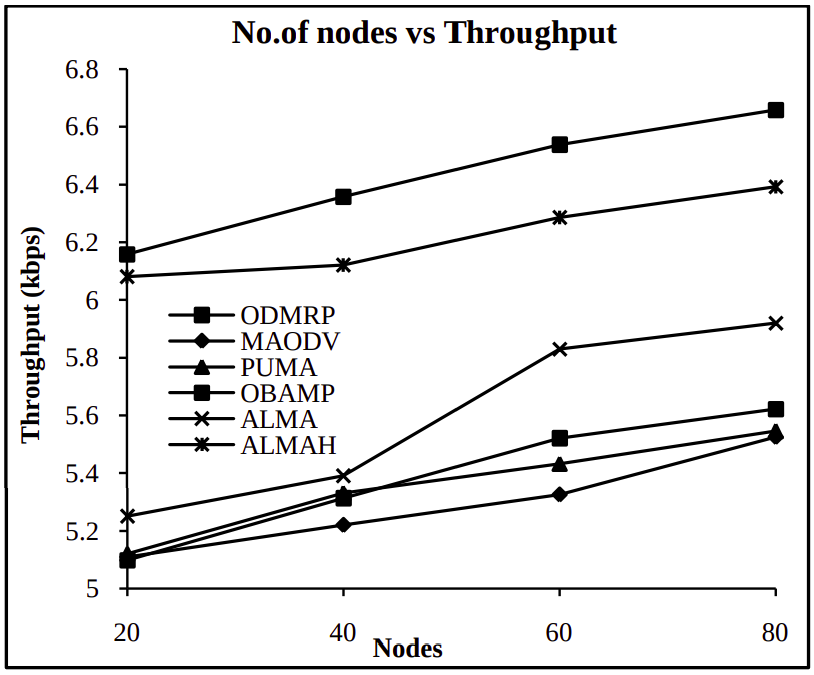
\includegraphics[width=7.8cm, height=7.8cm]{images/nodes-vs-throughput.png}
    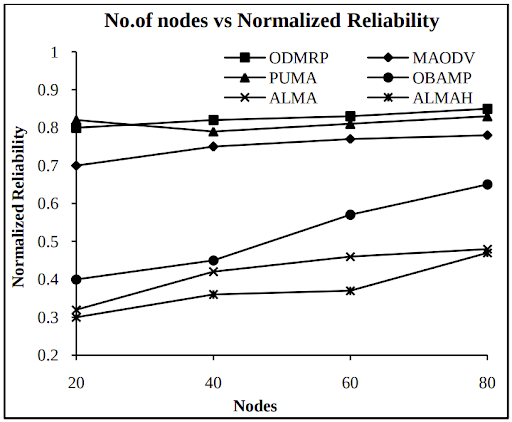
\includegraphics[width=7.8cm, height=7.8cm]{images/nodes-vs-reliability.png}
    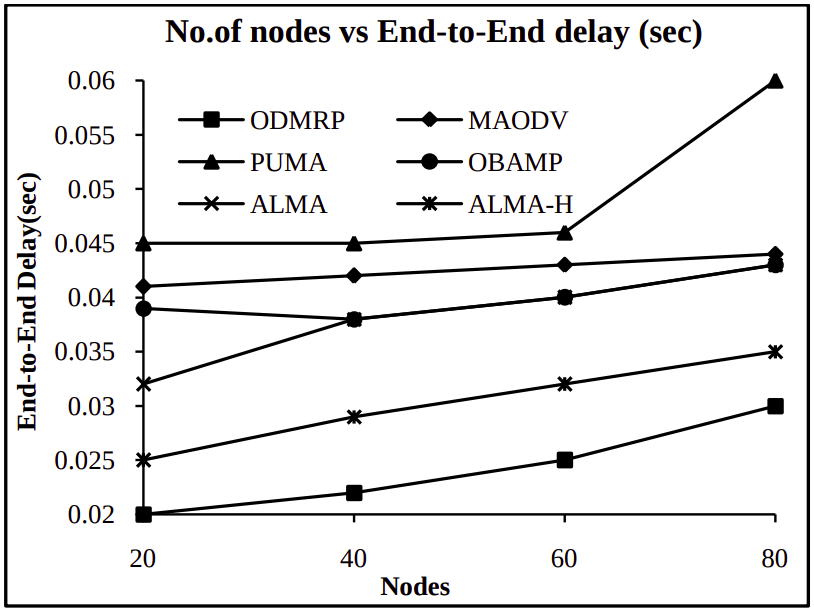
\includegraphics[width=7.8cm, height=7.8cm]{images/nodes-vs-e2edelay.png}
    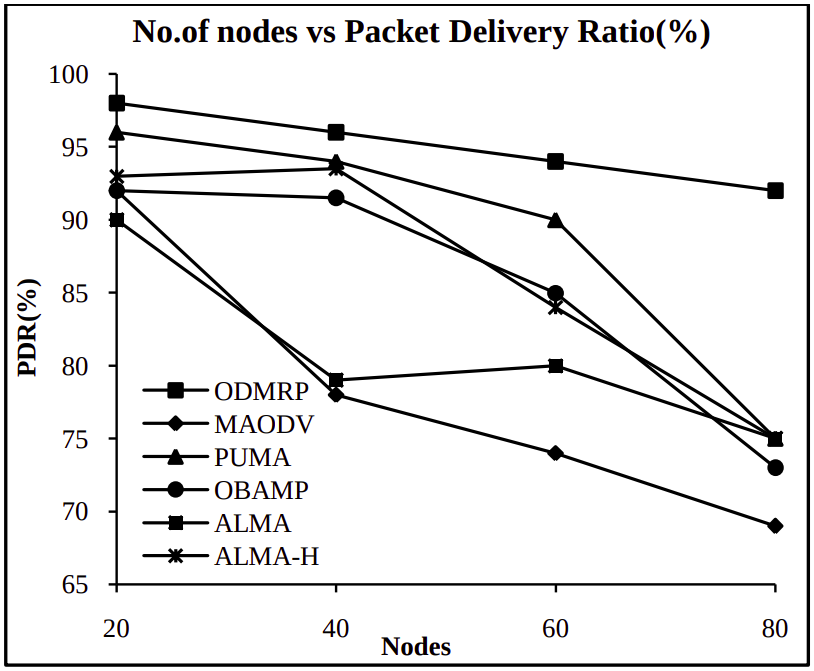
\includegraphics[width=7.8cm, height=7.8cm]{images/nodes-vs-pdr.png}
    \caption{Changing number of nodes vs reliability, throughput, delay and packet drop ratio}
    \label{fig:nodes-vs}
\end{figure}

\subsubsection{Varying the speed of nodes}

In this scenario the performance of the six protocols are measured for the four performance metrics by increasing the speed of nodes from 0 to 20 m/s with fixed number of nodes 80, the following graphs show the comparison between the performance of the six protocols.
\\
\\
Figure \ref{fig:mobility-vs} top left graph shows the simulation results of throughput versus the mobility speed in (m/s).
\\
We can see that the throughput decreases for all the six protocols as the mobility speed increases, and \acrshort{odmrp} has the best throughput as finding the route needs more routing traffic when speed increases. So less of the channel will be used to transfer data.
\\
\\
Figure \ref{fig:mobility-vs} top right graph shows the simulation results of reliability versus the mobility speed.
\\
We can see that by increasing the mobility speed \acrshort{odmrp} and ALMA-H have better reliability that the other protocols. This is because they have less transmission delay of messages.
\\
\\
Figure \ref{fig:mobility-vs} bottom left graph shows the simulation results of end-to-end delay versus mobility speed.
\\
When increasing the speed of the nodes, the topology changes frequently and then the probability of link breaking will increase. So additional route recovery process and route discovery process may be required. So as the speed increases, the end-to-end delay will also increase.
\\
\\
Figure \ref{fig:mobility-vs} bottom right graph shows the simulation results of packet delivery ratio versus mobility speed.
\\
The packet delivery ratio of all the protocols decreases when the speed increases, and \acrshort{odmrp} has better results than the other protocols.

\begin{figure}[!htbp]%
    \centering
    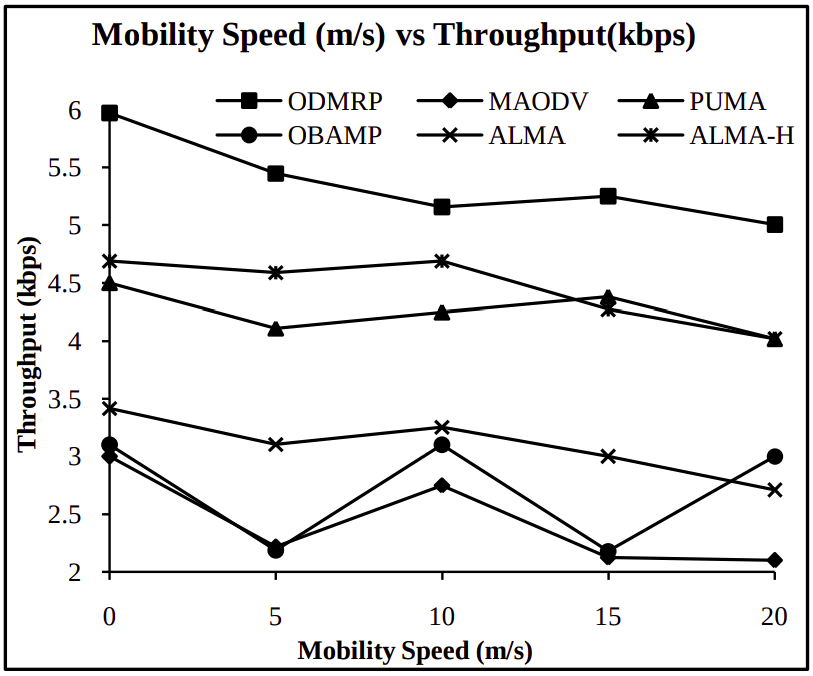
\includegraphics[width=7.8cm, height=7.8cm]{images/throughput-vs-mobility.png}
    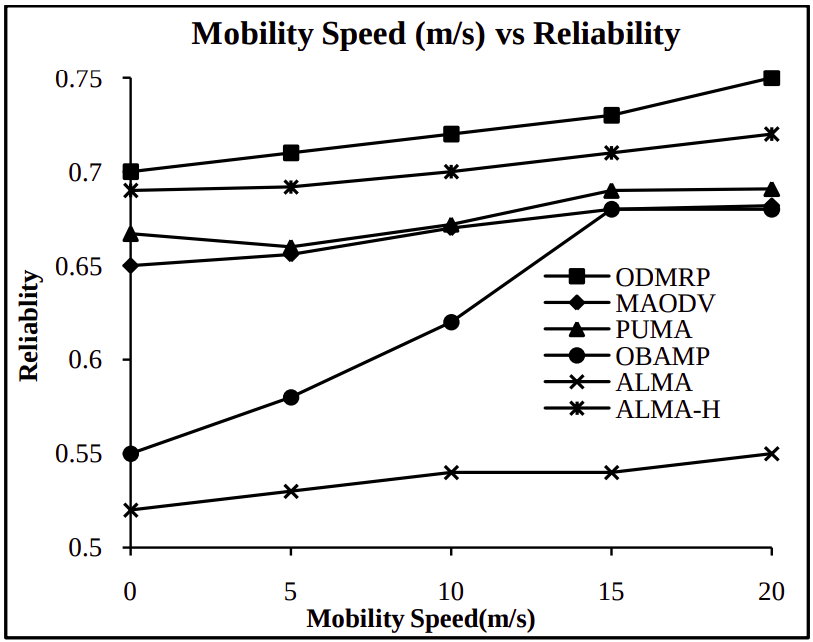
\includegraphics[width=7.8cm, height=7.8cm]{images/reliability-vs-mobility.png}
    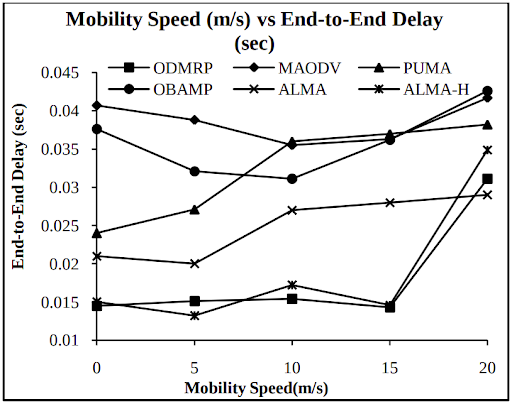
\includegraphics[width=7.8cm, height=7.8cm]{images/mobility-vs-e2edelay.png}
    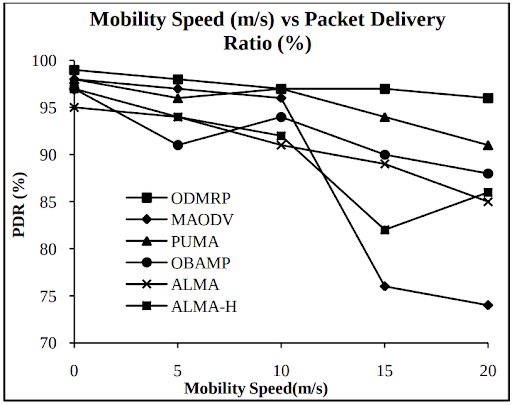
\includegraphics[width=7.8cm, height=7.8cm]{images/mobility-vs-pdr.png}
    \caption{Changing speed of nodes vs reliability, throughput, delay and packet drop ratio}
    \label{fig:mobility-vs}
\end{figure}

\section{Implemented Multicast Routing: \acrshort{odmrp}}
The Wireless Adaptive Mobility (WAM) Laboratory at the University of California, Los Angeles created the \acrfull{odmrp} \cite{ODMRP}, to reduce channel overhead and enhance scalability, \acrshort{odmrp} employs on-demand routing methods.
It constructs a forwarding mesh for each multicast group using the idea of a forwarding group, which is a collection of nodes responsible for passing multicast data.
The disadvantages of multicast trees in mobile wireless networks, such as inconsistent connectivity, traffic concentration, frequent tree reconfiguration, and non-shortest path in a shared tree, are addressed by maintaining and utilizing a mesh instead of a tree.
To keep multicast group members, a soft-state technique is used.
To quit the group, no specific control message is necessary.
We feel that \acrshort{odmrp} is more appealing in mobile wireless networks because of the reduced channel/storage overhead and the relaxed connection.
The advantages of \acrshort{odmrp} are highlighted by the features listed below.

\subsection{\acrshort{odmrp} Overview}
\acrshort{odmrp} is a mesh-based multicast scheme that employs a forwarding group idea to ensure that only a subset of nodes forwards multicast packets, rather than a traditional tree-based multicast scheme, It uses on-demand processes to create routes and manage multicast group membership dynamically.
\acrshort{odmrp} is ideally suited for ad hoc wireless networks with mobile hosts in which bandwidth is restricted, topology changes often and quickly, and power is limited.
\\
\\
The Query and Reply stages make up the \acrshort{odmrp}.
A packet Join Query is broadcast by source on a regular basis.
Every node in the network saves the upstream node address in the route database and rebroadcasts the packet to its neighbor nodes when it receives a non-duplicate Join Query packet via the reverse path technique.
When a multicast receiver receives a Join Query packet, it generates and transmits a Join Reply to its neighbors.
\\
Following the learned reverse path, this Join Reply packet is sent all the way back to the source, and the nodes on the reverse path become the forwarding group.
The following is how data is provided by the forwarding group nodes:
The source broadcasts data packets, while nodes in the forwarding group rebroadcast non-duplicate packets so that packets can be transmitted to recipients.
The forwarding group is a collection of nodes that are in charge of transmitting multicast data, thus establishing a mesh between all senders and receivers.
When a new node wishes to become a receiver in a multicast group, it waits for the next Join Query and replies with a Join Reply packet.
If a receiver becomes detached from the forwarding mesh owing to mobility, it must also wait for the next Join Query flooding.
\\
Without a local route recovery mechanism, \acrshort{odmrp}'s frequent route refresh and redundant forwarding maintain a high packet delivery ratio.
A soft-state technique is used in \acrshort{odmrp} to keep track of multicast group members; no explicit control messages are needed to join or exit the group.
A source node simply stops delivering a Join Query when it has no more packets to send.
If a receiver wishes to leave a multicast group, it does not answer to the multicast group's Join Query.
\\
If a forwarding node does not get the Join Reply after reaching a timeout that is a multiple of the refresh interval, it becomes a non-forwarder. 
\\
\\
After comparison to the previous routing protocols and other protocols using the four performance metrics: throughput, reliability, end-to-end delay and packet delivery ratio under two conditions: increasing the number of nodes and increasing the speed of the nodes. We found that In all cases, \acrshort{odmrp} outperforms the other multicast routing protocols, leading to the conclusion that \acrshort{odmrp} is effective and efficient in highly dynamic conditions and scalable to numerous multicast nodes, as for route discovery and maintenance, \acrshort{odmrp} uses periodic network-wide flooding. The purpose of this design is to guarantee robustness in the face of mobility and poor wireless connection propagation, and this feature would be very useful especially in rugged environments.

The reasons we chose \acrshort{odmrp} as our multicast routing protocol are summarized in the following points:

\begin{itemize}[itemsep=1pt, topsep=5pt]
\item The ability to route unicast traffic.

\item Low overhead in terms of channels and storage.

\item Use of the most recent shortest routes.

\item The ability to withstand host movement.

\item Reliable route and forwarding group development.

\item Wireless settings' broadcast nature is used.

\item Maintenance and exploitation of multiple redundant paths.

\item Scalability through the use of effective flooding.

\item The protocol's extensibility.

\item Limited power usage.
\end{itemize}

There is always room for optimization. \acrshort{odmrp} is one of the best multicast routing protocols but with some modifications as We did in broadcasting the join reply packets by using the filled tables to only sending the join reply packet to the upstream nodes, it also can be optimized further by other extendable versions of \acrshort{odmrp}:
\begin{itemize}[itemsep=1pt, topsep=5pt]
    \item E-\acrshort{odmrp} version of \acrshort{odmrp} with adaptive refresh. Rather than mobility prediction, receivers report connection breakages, which drives adaptation. A basic local recovery is easily incorporated with the adaptive refreshing method. In light load, EODMRP \cite{EODMRP} may have a slightly lower packet delivery ratio than \acrshort{odmrp}, but it may be better in high loads.
    \item RODMRP \cite{RODMRP} which seeks to be robust to network or node failures and to provide a continuous multicast service for live data streaming.
    \item It also could be extended to work with zones.
\end{itemize}

% @INPROCEEDINGS{MAODV,

%   author={Zhong, Mingyang and Fu, Yunqing and Jia, Xinqiang},

%   booktitle={2011 International Conference on E-Business and E-Government (ICEE)}, 

%   title={MAODV multicast routing protocol based on node mobility prediction}, 

%   year={2011},

%   volume={},

%   number={},

%   pages={1-4},

%   doi={10.1109/ICEBEG.2011.5881805}}

\chapter{System Design and Architecture}
\label{ch:system-design}

This chapter describes the following in detail:
\begin{itemize}[itemsep=1pt, topsep=5pt]
    \item All the system modules.
    \item The flow of data between modules.
    \item Modules' functionalities.
    \item Design constraints.
    \item The decisions we took about the modules' functionalities.
\end{itemize}

The overall system could be broken down to mainly 3 components:
\begin{itemize}[itemsep=1pt, topsep=5pt]
    \item The Router: Implements unicast, multicast and broadcast within a control plane and forwarding plane.
    \item Unit \& \acrfull{cmd}: 2 applications for tactical teams communications.
    \item Testbed: Set of scripts, kernel modules, programs and \acrfull{gui} for system testing and development which emulates the \acrfull{hw} and simulates the environment in which the system will be deployed.
\end{itemize}

This chapter discusses the first 2 modules, while the testbed is discussed completely in chapter \ref{ch:system-testing}, because it's not part of the final deployed system, but rather built for testing purposes.

\section{Overview and Assumptions}
Units are soldiers who are deployed in the operations field, while commanders are in their vehicles or buildings sending commands to the soldiers/officers and monitoring their locations and watching streaming and audio recording from soldiers and sending and receiving code messages to the deployed soldiers.

Commanders have powerful devices, while units have low-end devices with low range for maximum battery conservation.

\subsection{Reliability}
The following must be delivered reliably (with guarantee of delivery):
\begin{itemize}[itemsep=1pt, topsep=5pt]
    \item Code messages.
    \item Audio messages.
\end{itemize}

The following can be delivered unreliably (*no* guarantee of delivery):
\begin{itemize}
    \item Video streams.
    \item Position and heartbeat messages (minimum 80\% delivery success rate).
\end{itemize}

\subsection{Speed}
The system allows nodes to communicate with low latency and high throughput.

\subsection{Security}
\begin{itemize}[itemsep=1pt, topsep=5pt]
    \item All transmitted data are encrypted. Including the headers.
    \item Authentication is required for accessing command center by its \acrshort{ui}.
    \item Units don't persist any data, messages self-destruct after receiving and playing them.
\end{itemize}

\section{System Architecture}
% The aronal fieldchitecture of your system should be given in this section. This architecture should be first represented as a block diagram (subsection 5.2.1), which clarifies different project modules and the connections between them. You may add more subsections to properly explain your design. If possible, flowcharts are better included to ensure that the big picture and the interaction between different modules are very clear to the reader. Thereafter, each module should have a separate subsequent section to clearly describe and discuss it.
The system is composed of devices (\textit{nodes}) running Linux-based operating systems and have certain programs running in them.

\subsection{Nodes}
All nodes are provided with wireless communication modules that follow \texttt{IEEE 802.11} standards for wireless communications.

There are 2 types of nodes:
\begin{enumerate}[itemsep=1pt, topsep=5pt]
    \item Units.
    \item Command Centers (shortened as \textit{\acrshort{cmd}}.)
\end{enumerate}

\subsubsection{Units}
\label{subsubsec:units-dev}
Units (software) run on devices with deployed units (persons) in the operation field, the single device has:
\begin{itemize}[itemsep=1pt, topsep=5pt]
    \item LCD screen, to show the code messages and device state (battery and location and number of received audio messages.)
    \item Helmet video camera. Could be mounted on a vehicle if the device runs on one.
    \item Audio input from microphone with button to start recording.
    \item Audio output, to hear received recorded messages.
    \item Keypad, to enter code messages.
    \item GPS (or any other position detection system.)
    \item One heartbeat sensor, that streams the beats per minutes of the person who operates the device.
\end{itemize}

The unit device has the following features:
\begin{itemize}[itemsep=1pt, topsep=5pt]
    \item Low power consumption.
    \item Running on battery.
    \item Low wireless range.
    \item High mobility.
    \item Operated by one person.
\end{itemize}

A unit device has 2 programs:
\begin{itemize}[itemsep=1pt, topsep=5pt]
    \item Router: Implements routing protocol.
    \item Unit Client Daemon: Connected to device hardware and network interface and provide all unit features.
\end{itemize}

\subsubsection{Command Centers}
High-end computers at the command and control centers, accessed by units leaders.

The command center device has the following features:
\begin{itemize}[itemsep=1pt, topsep=5pt]
    \item Capable of high power consumption.
    \item Powerful CPUs.
    \item Big storage and RAM.
    \item Operated by multiple people with multiple wide screens.
    \item Wide wireless range.
    \item Installed nearby the operation field, and has a connection to devices in the field.
    \item Low (or zero) mobility.
\end{itemize}

A command center computer has 3 programs:
\begin{itemize}[itemsep=1pt, topsep=5pt]
    \item Router: Implements routing protocol, same router as in unit devices.
    \item Command Client Daemon: Exposes an interface to \acrshort{ui} program, connects to units clients and handles all communication with units.
    \item Command Client \acrshort{ui}: Connects to Command Client Daemon, shows all data in the daemon and controls it.
\end{itemize}

\subsection{Block Diagram}
\begin{figure}[!htb]
    \centering
    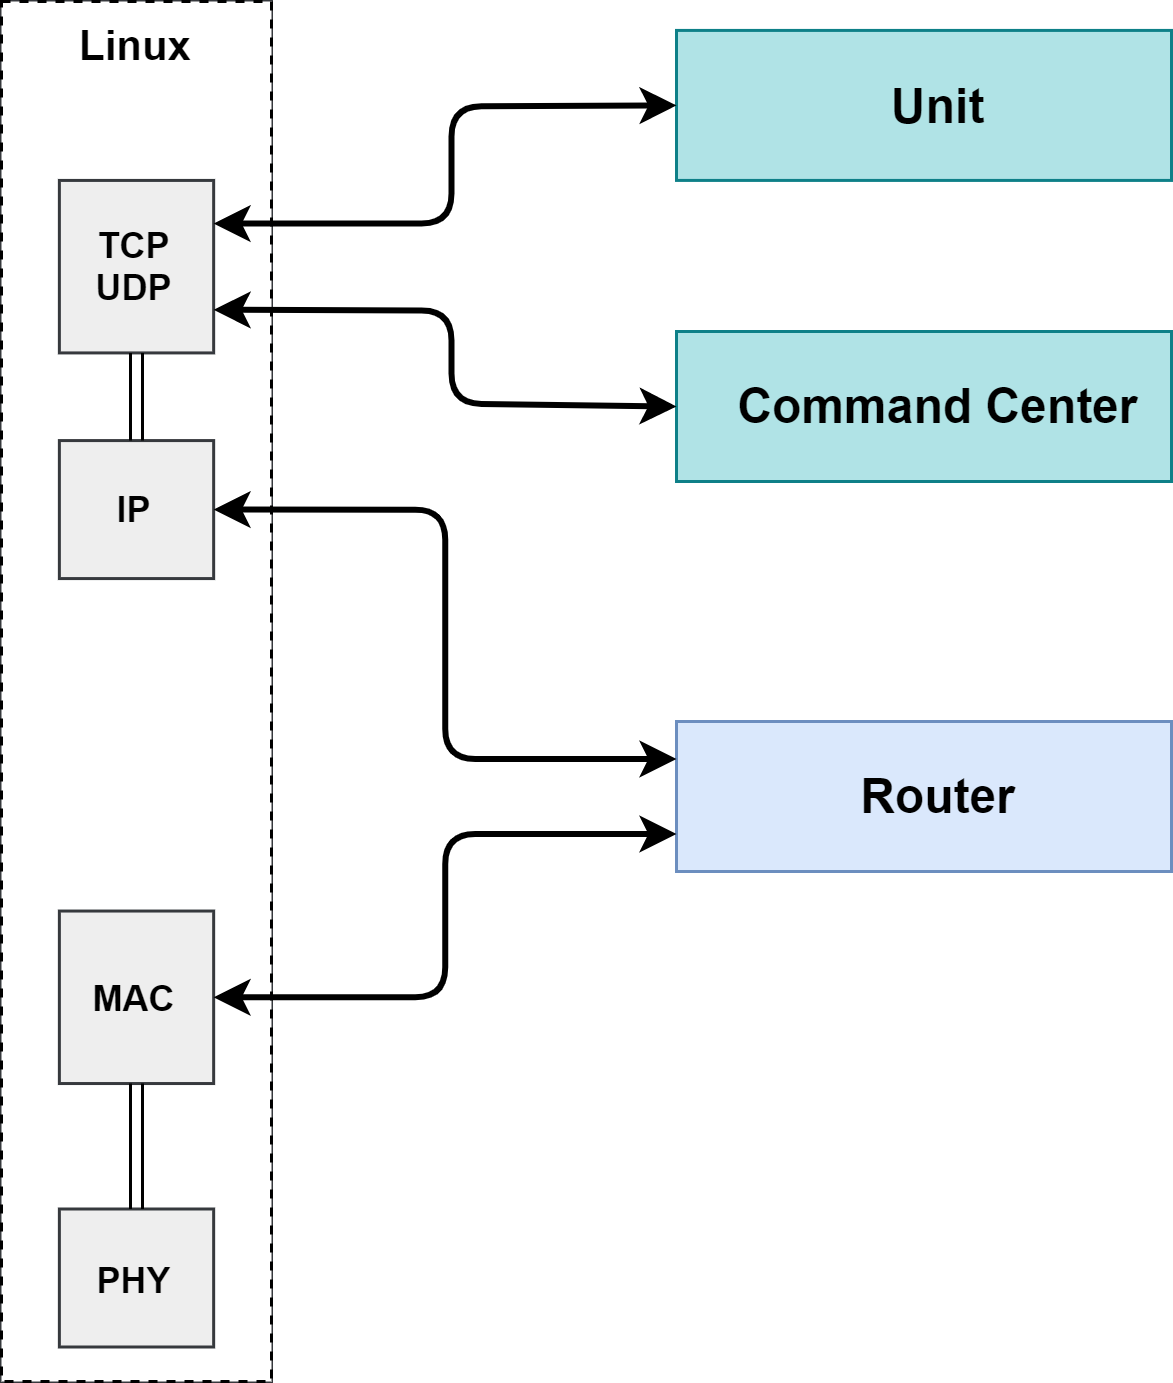
\includegraphics[width=0.8\linewidth]{images/overall-system.png}
    \caption{Overall System}
    \label{fig:overall-system}
\end{figure}

Figure \ref{fig:overall-system} shows the overall \acrshort{caian} system modules.

Unit or Command Center are applications that communicate directly with the TCP/UDP standard OS interface.
You would only use unit or command center on one device.
They are not aware of the router that sits on the bottom, this means they should work on localhost, which we already do for testing purposes to isolate system modules.

The router sits in the bottom, it's backward compatible with the Linux kernel network stack design, this means that programs in the application layer won't change when using the router.
The router takes packets going out of the system, and encrypts the packet and wraps it with our own headers and decides the forwarding of the packet.
Then the router puts back the packet in the \acrshort{mac} layer, so it's sent to the destination.

In the testing environment, as we will detail in chapter \ref{ch:system-testing}, we will isolate routers in each container with its own network stack, and create either a unit or command center program depending on the node type.

\section{The Router}
Routing is the process of filling the forwarding tables, while forwarding is the process of taking a packet and deciding the destination from the forwarding table.
The router is the main component of the project, the rest are applications that show the effectiveness of the router.
The router is backward compatible with Linux's standard network stack and works completely in the user space.

The router enables all programs and kernel modules that communicate with the \acrshort{ip} layer to run over an ad-hoc network transparently without changing any line of code.

\subsection{Functional Description}
The router takes the packet after wrapping the TCP/UDP/ICMP with IP headers, and wraps it with its packet \acrfull{zid} for interzone forwarding and encrypts the whole packet.
The router also encrypts all packets including control packets before them leaving the device.
This stops any device that doesn't share the same credentials from participating in the network and ensures the security of the communications.

The router exchanges control packets to build the topology that may be used for forwarding when a packet is available.

The router provides unicast, multicast and broadcast services to the upper layers based on \acrshort{ip} address patterns.

\subsection{Modular Decomposition}
Figure \ref{fig:router-modules} shows the modules of the router in detail.

\begin{figure}[!hbf]
    \centering
    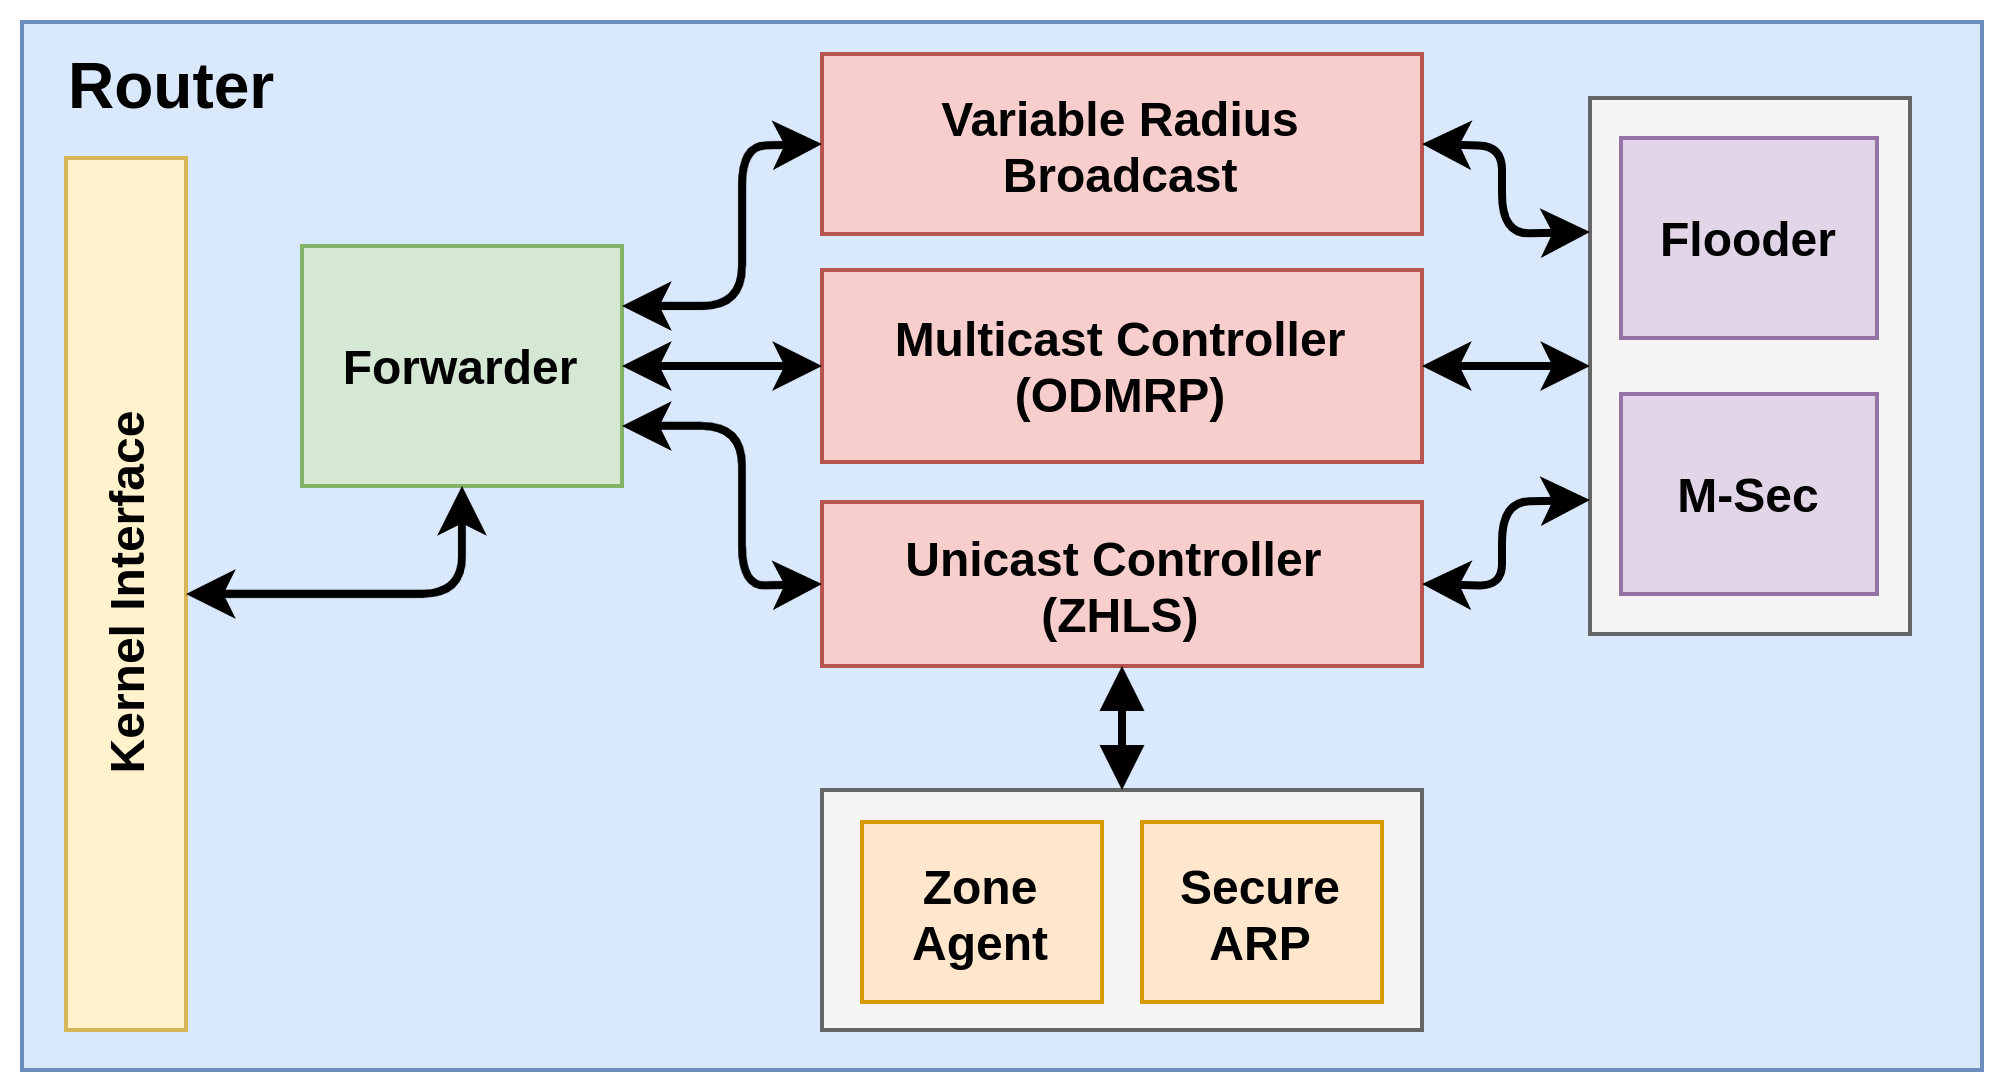
\includegraphics[width=14cm]{images/router-modules.png}
    \caption{The Router Modules}
    \label{fig:router-modules}
\end{figure}

Broadcast routing implements a new protocol we introduced called ``Variable Radius Broadcast'' (VRB), which limits the broadcast to a given geographical radius.
Unicast routing implements the ``Zone Hierarchical Link State Routing'' (\acrshort{zhls}) protocol, which solves the scalability requirements for the routing.
Multicast routing implements the infamous protocol ``On Demand Multicast Routing'' (ODMRP) protocol.

All the three routing protocols are implemented in the control plane.
They fill different kinds of forwarding tables suited for each protocol.

In the forwarding (data) plane there is the forwarder which is a complex module that takes packets leaving and entering the device and either forwards them or injects them back based on the 3 protocols' forwarding tables and has channels with the control plane to kick reactive routing decisions, like finding a zone for destination or starting the process of sending join query messages for ODMRP.

\subsubsection{Kernel Interface} 
The router reads and writes packets from the kernel in 3 ways:
\begin{itemize}[itemsep=1pt, topsep=5pt]
    \item Netfilter Queue: Used to steal packets from the kernel. They were designed in mind for firewall and deep-packet-inspections applications, but it suited our use case. The kernel gives us each packet leaving the device, and we drop them and deal with them ourselves and send it to the device driver.
    \item Packet Sockets: Used to read/write packets at the device driver, writing to it send a packet out the device.
    \item Raw Sockets: Used to inject packets into the \acrshort{ip} layer after receiving them from the 
\end{itemize}

\subsubsection{Forwarder}

The forwarder constitutes our data plane. It is where all the data packets pass and get routed. The forwarder listens to packets coming from the \acrshort{ip} layer and packets coming from the \acrshort{mac} layer. Packets coming from the \acrshort{ip} layer are packets originating at the current node, while packets coming from the \acrshort{mac} layer are packets arriving from other nodes, either addressed to the current node or to another destination. The forwarder is responsible for controlling the flow of those data packets. Figure \ref{fig:forwarder-data-flow} shows how the data flows through the forwarder.

\begin{figure}[!htb]
    \centering
    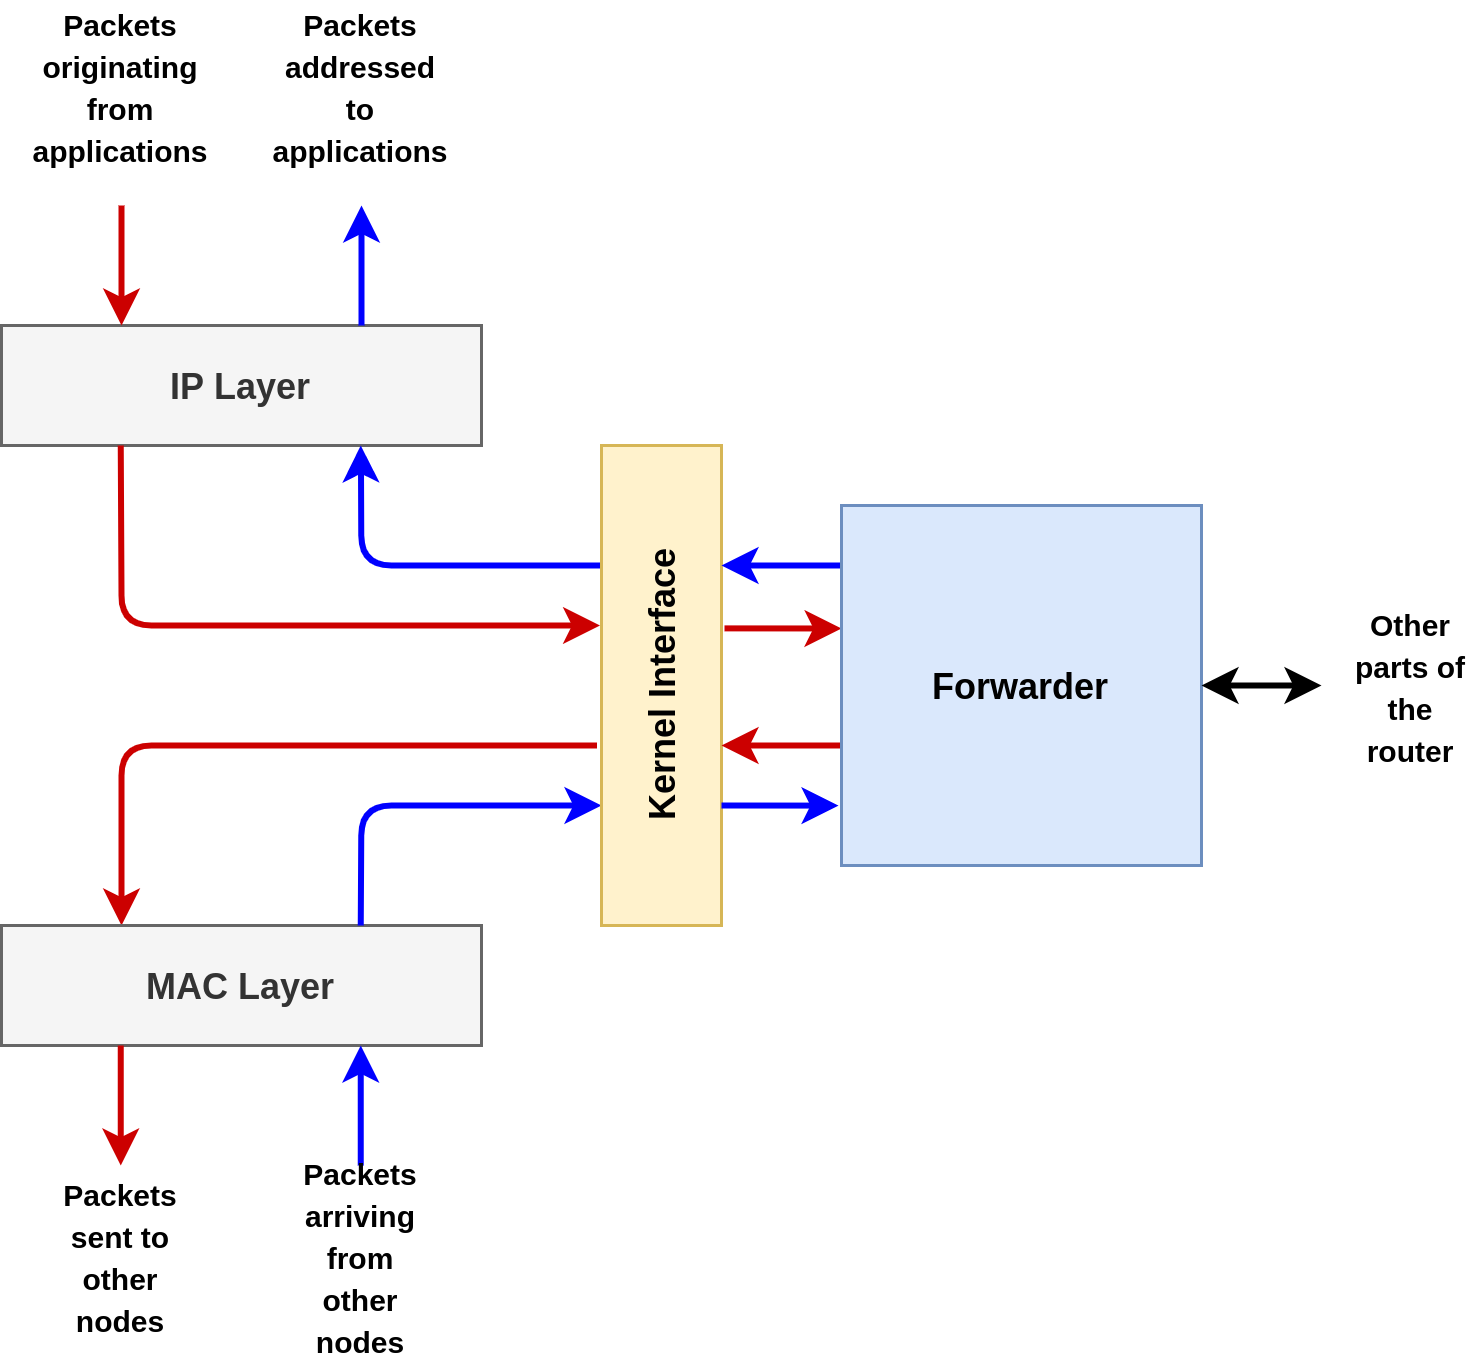
\includegraphics[width=0.9\linewidth]{images/forwarder-data-flow.png}
    \caption{Data Flow Through the Forwarder}
    \label{fig:forwarder-data-flow}
\end{figure}

When the forwarder receives data from the \acrshort{ip} layer, it first checks the type of routing required for the \acrshort{ip} packet depending on the destination \acrshort{ip} address, which can be unicasting, multicasting, or broadcasting:
\begin{itemize}[itemsep=1pt, topsep=5pt]
    \item \textbf{Unicasting}
    \begin{itemize}[itemsep=1pt, topsep=5pt]
        \item The destination zone is found through the unicast controller.
        \item A \acrshort{zid} header is constructed and prepended to the packet.
        \item The next hop is determined through the unicast forwarding table constructed by the unicast controller.
        \item The packet is encrypted and send to the next hop through the \acrshort{mac} layer.
    \end{itemize}
    \item \textbf{Multicasting}
    \begin{itemize}[itemsep=1pt, topsep=5pt]
        \item The next hop is determined through the multicast forwarding table constructed by the multicast controller.
        \item The packet is encrypted and send to the next hop through the \acrshort{mac} layer.
    \end{itemize}
    \item \textbf{Broadcasting}
    \begin{itemize}[itemsep=1pt, topsep=5pt]
        \item The packet is encrypted and sent through the variable radius broadcast handler.
    \end{itemize}
\end{itemize}

The forwarder uses different listeners to receive unicast, multicast, and broadcast packets from the \acrshort{mac} layer. The packets are differentiated using a unique ethertype used by the forwarder for each packet type. 

When the forwarder receives a unicast packet from the \acrshort{mac} layer, it decodes, decrypts and validates the \acrshort{zid} and \acrshort{ip} headers. The forwarder then checks whether the current node is the destination of the packet. If so, the packet is sent to the \acrshort{ip} layer. Otherwise, the forwarder checks if the destination node lies within the current zone's node through the \acrshort{zid} header. If it does, the forwarder checks the unicast forwarding table for the next hop for the destination node. Otherwise, the forwarder checks the unicast forwarding table for the next hope for the destination zone. The \acrshort{ip} header is then reconstructed to update the TTL and checksum, and the packet is forwarded to the next hop though the \acrshort{mac} layer. An interesting case is when a packet reaches its destination zone, but the forwarder cannot find the destination node in its zone. This may occur due to the mobility of the nodes, as the node may have left the zone after the packet was sent from the source. In this case, the forwarder uses the unicast controller to find the new zone of the destination, and reconstructs the \acrshort{zid} header with the new destination zone.

When the forwarder receives a multicast packet from the \acrshort{mac} layer, it decodes, decrypts and validates the \acrshort{ip} header. The forwarder then checks to see whether the current node is a member of the destination multicast group. If so, the packet is sent to the \acrshort{ip} layer. Regardless of whether the current node is a member, the packet may need to get forwarded according to the structure of the multicast mesh. The forwarder checks if it should forward the packet using the multicast forwarding table. If it should, it reconstructs the \acrshort{ip} header to update the TTL and checksum, and the packet is forwarder to the next hop.

\subsubsection{Variable Radius Broadcast (VRB)}
Research in ad-hoc routing gave most of its attention to unicast protocols, while broadcast and multicast were left in the dark.
Broadcasting in infrastructure networks uses the subnetting mechanism to limit the broadcasting and put boundaries, while this is most effective to decide who participates in broadcasting, but this is not applicable to ad-hoc networks because there are no subnets otherwise moving devices will be assigned different IPs each time they change cluster and this will disrupt applications logic and break the backward compatibility.

Given that \acrshort{zhls} already requires geographical locations to be maintained and shared, we figured out a way to put boundaries on the broadcasting using the current location of each device.

The protocol is simple, you know which zone you are in, when some device wants to broadcast a message it will put the broadcasting radius in the lowest byte of the destination \acrshort{ip} while setting the rest of the bits to 1.
when a device receives a broadcast a message it will check the src zone and the radius and its zone and calculates the radius between its zone and the src zone, if the calculated radius is bigger than the given radius (in the destination \acrshort{ip}) it won't forward the packet anymore otherwise it floods the message.

\subsubsection{Flooder}
Flooder is a component of any routing system that distributes every incoming packet via every outbound connection except the one from which it originated. Because \acrshort{caian} uses wireless channels as a physical layer to suit the nature of tactical teams on battlefields, and because wireless networks are broadcast by their inherent nature, this implies two important aspects in our flooding approach implementation:

\begin{itemize}[itemsep=1pt, topsep=5pt]
    \item There is no need to figure out which outgoing connection the incoming packet should be sent to; simply broadcast it.
    \item The need for a flood control method in order to avoid transmitting duplicate packets and endless recycling of the same packet.
\end{itemize}

Because \acrshort{caian} uses a zone-based routing approach for unicasting, we needed to manage the flooding area, therefore we built two flooders: a zone flooder and a global flooder. The zone flooder is primarily used to flood intrazone LSR control messages, whereas the global flooder was used by the unicast algorithm to flood interzone LSR control messages, and it was also used by the multicast algorithm.

Before flooding any packet, it must contain a \acrshort{zid} header (not required in global flooder) and a flooding header that is shown by Figure  \ref{fig:flood-header}. 

\begin{figure}[!htb]
    \centering
    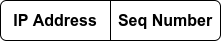
\includegraphics[scale=1]{images/flood_header.png}
    \caption{Flooding Header}
    \label{fig:flood-header}
\end{figure}

The header fields are as follows:
\begin{itemize}[itemsep=1pt, topsep=5pt]
    \item \textbf{\acrshort{ip} address:} The \acrshort{ip} address of the sender.
    \item \textbf{Seq Number:} The sequence number of that packet from that source.
\end{itemize}

Seq. number is used to control the packet flooding in the network and to prevent recirculation of the same packet indefinitely. So for any router to accept an incoming packet and flood it to all neighbors, it must satisfy three conditions:

\begin{itemize}[itemsep=1pt, topsep=5pt]
    \item It must not be flooded by the receipt router itself. 
    \item It must be flooded by a router that exists in the receipt router zone.
    \item It must have a sequence number that is higher than the latest one stored for that source.
\end{itemize}

It is obvious that the second condition is only required by the zone flooder.

According to the preceding definition, each router must keep a sequence number for each other router in the zone (or the network in the case of global flooding) that has the value of the sequence number attached with the most recent packet from that source. Each entry in the preceding flooding table has a timer connected to it in addition to the sequence number. Once the timer goes off, the entry must be deleted immediately. This timer will allow accepting packets from a router that has gone down for whatever reason and reset its sequence number to zero.

\subsubsection{M-Sec}
M-Sec stands for ``MANET Security'' which is the encryption layer we introduced in the router.
It encrypts all outcoming packets (including their headers) and decrypts all incoming packets.

M-Sec uses AES256-CFB for its speed and no found vulnerabilities yet.
We didn't choose asymmetric encryption like that used in IPsec because of the problem of certificates sharing and signing, which introduces unwanted centralization which weakens the security of the whole system in case the central authority was compromised.
Also, central authorities add to the complexity of the system, which makes it harder for huge organizations like the military and any tactical teams in general to adapt to.

M-Sec uses passphrase for its key derivation, which is done using pbkdf2 with 4096 iterations and a fixed salt.
The reason to use passphrase is to integrate seamlessly with the military way of securing communications, which they have been trained to for decades.
This enables \acrshort{caian} to be a drop-down replacement for traditional radio systems without more training.

When we encrypt a packet, we encrypt each header on its own, this enables quick decryption for the needed header to decide its destination in the forwarding plane and in case we need to update the header's data like TTL and needed to recalculate the checksum, no need to encrypt the whole packet.

Using CFB mode enables the packet to be encrypted without increasing its size because it's a stream mode.
It was also chosen among other stream modes because of its capability to detect tampering with the packet, in case someone changed one bit the whole stream will change completely which will be detected easily either by the \acrshort{ip} header checksum or version or TCP/UDP/ICMP length or checksum or the application layer.
This provides authentication besides confidentiality.

\section{Unicast Controller}
\subsection{Functional Description}
The unicast controller is in charge of one-to-one transmission between two network nodes; that is, one sender and one receiver, each with an \acrshort{ip} address. At every node, it creates a forwarding table, which includes the best next-hop to forward a packet to for each possible destination. Collectively, this constitutes finding a path from every possible source to every reachable destination. As indicated in the preceding section, we believe \acrfull{zhls} is one of the best hybrid unicast protocols for this task. As a result, we chose it as our unicast routing protocol.

\subsection{Modular Decomposition}

\begin{figure}[!htb]
    \centering
    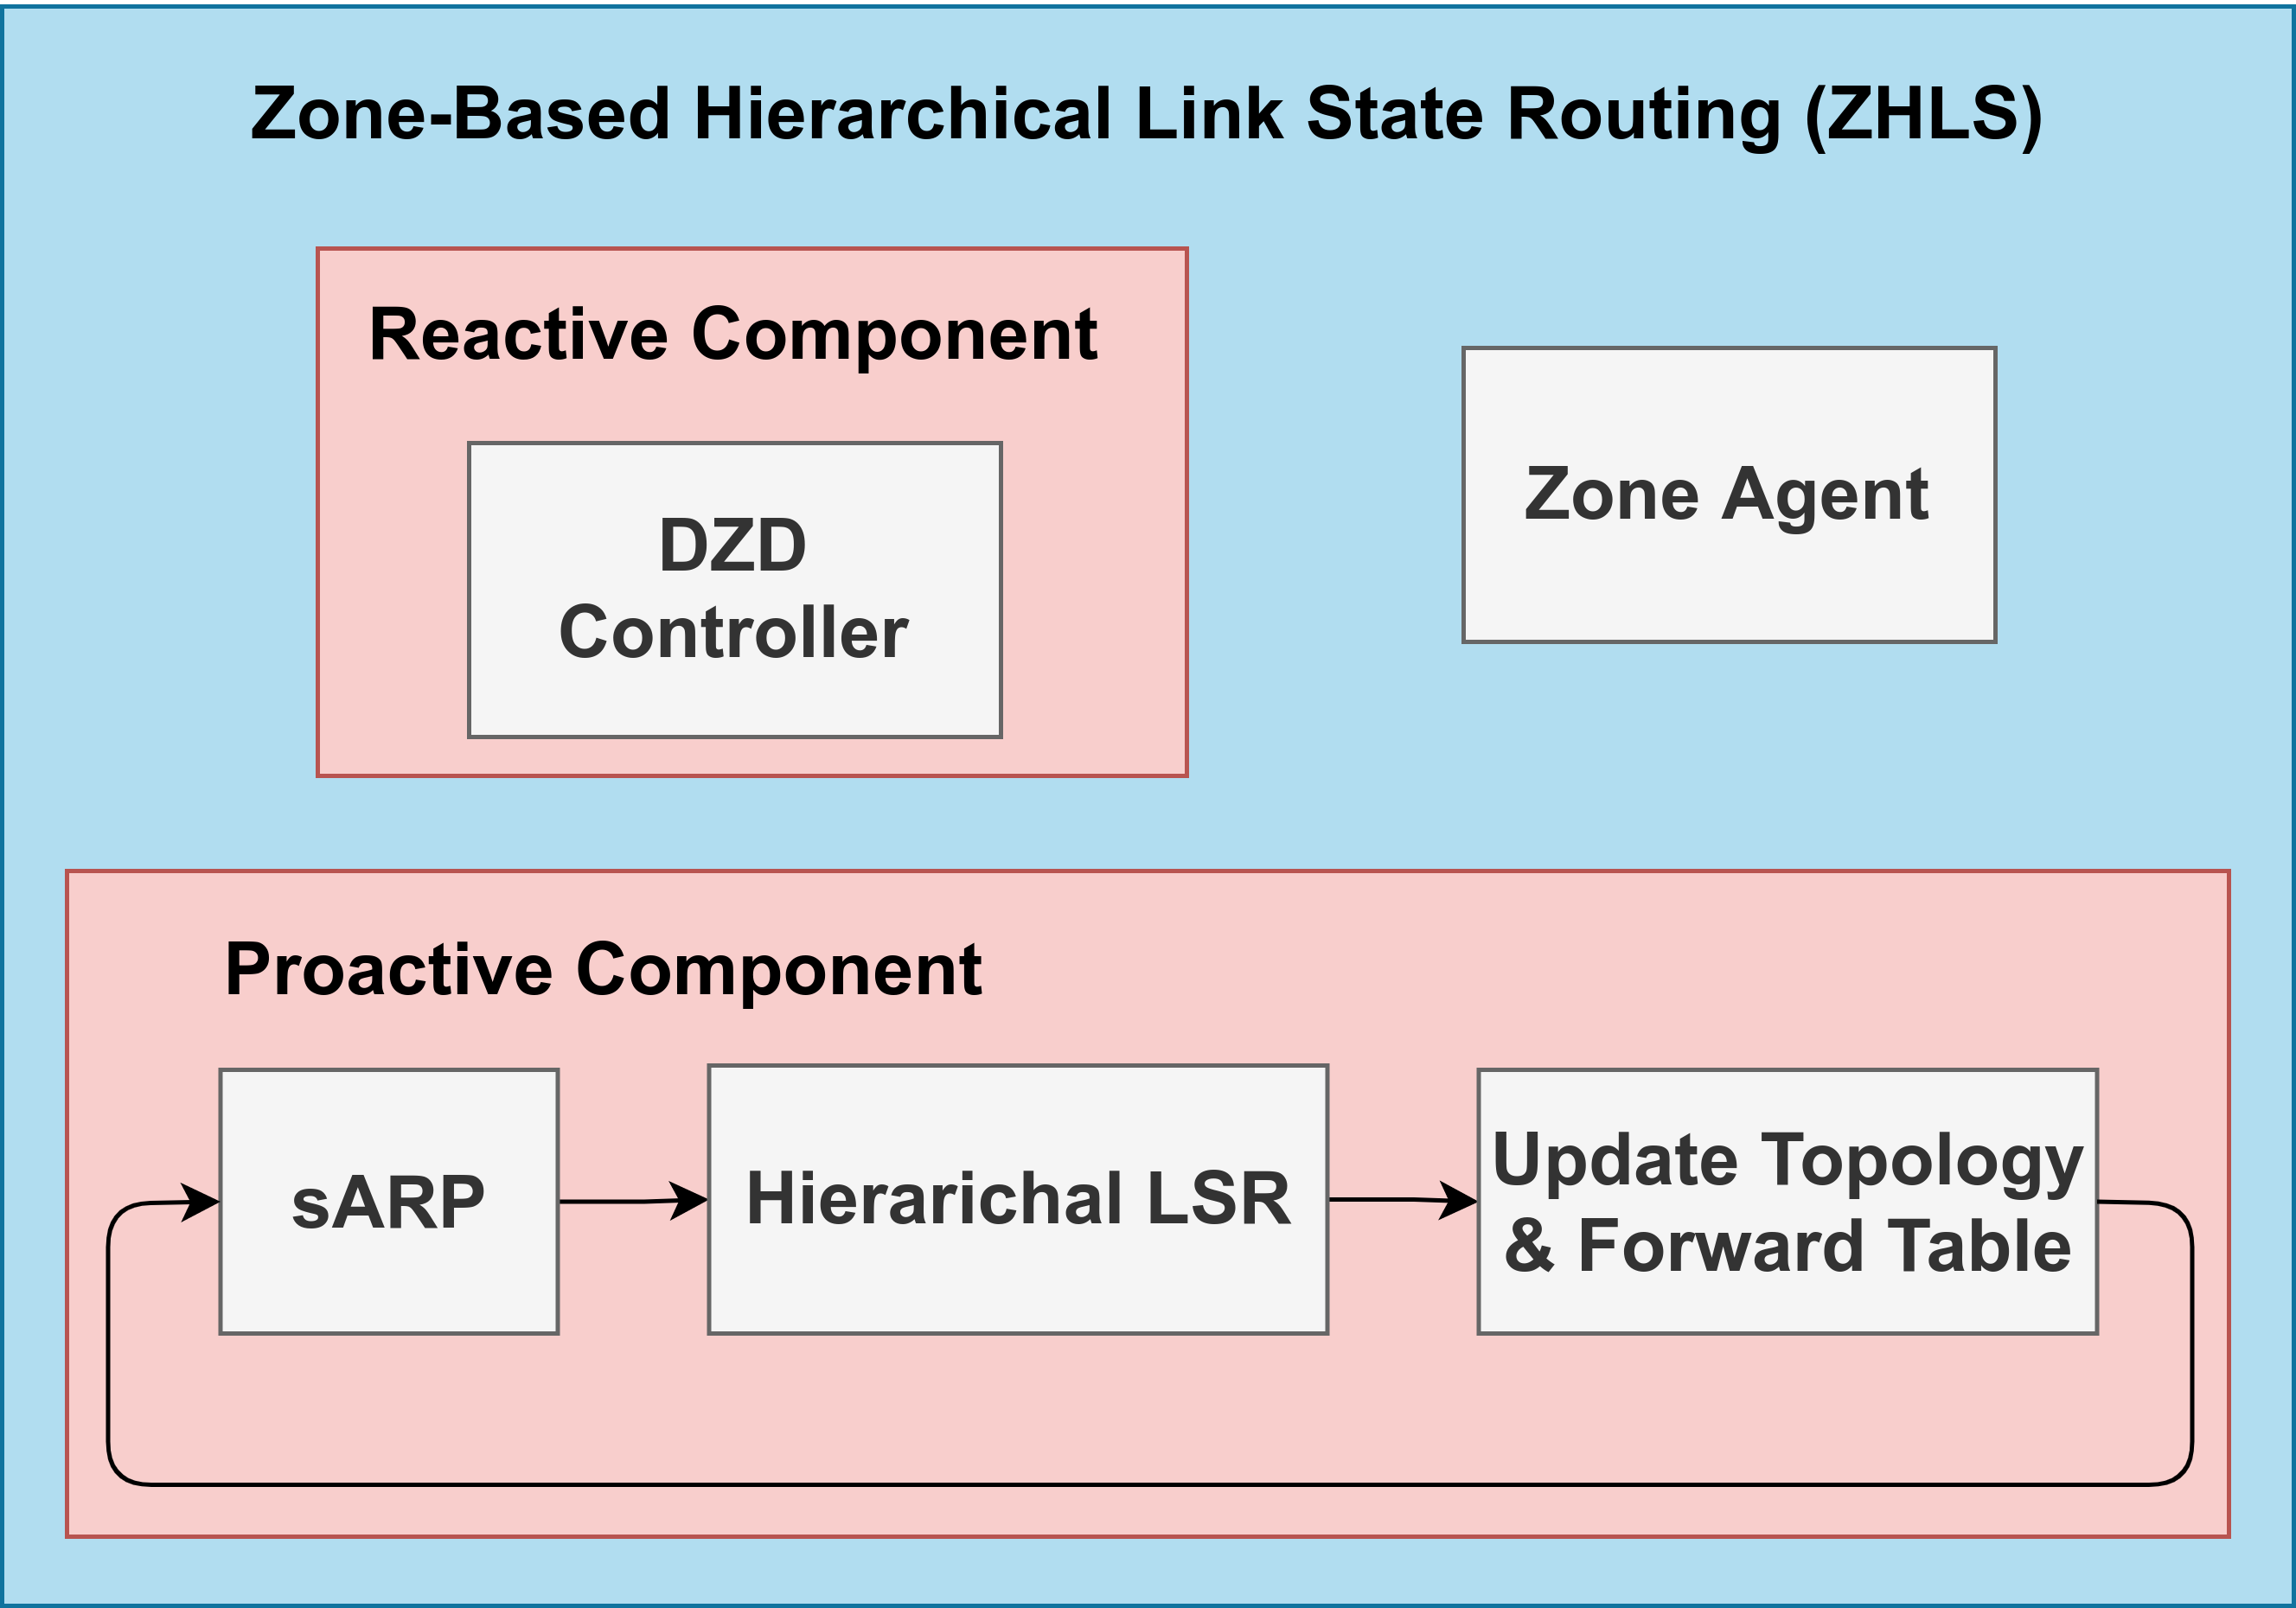
\includegraphics[width=\linewidth]{images/zhls-modules.png}
    \caption{\acrshort{zhls} Modules}
    \label{fig:zhls-modules}
\end{figure}

\acrfull{zhls} may be divided into proactive and reactive components due to the fact that it is a hybrid routing protocol. In addition, there is a module that is in charge of zone administration. \acrshort{zhls} modules can be show in Figure  \ref{fig:zhls-modules} 
The proactive component of the \acrshort{zhls} is the component that is repeated on a regular basis to gather and store up-to-date routing information about the topology and state of zones. It does this by following three consecutive protocols: collecting data about neighbor nodes and zones which is done using Secure ARP protocol, flooding this information over the network using LSR packets, and updating the hierarchical topology and forward table with the flooded information. This procedure is done on a regular basis to maintain the routing information updated. 
The reactive component of the \acrshort{zhls} is the component that is responsible for discovering the destination zone as soon as data is ready in the source and the destination \acrshort{ip} doesn't exist in the source forwarding table (the destination is in a different zone). The protocol that is used for this task is called Destination Zone Discovery (DZD). 
Finally, the Zone Agent module is in charge of managing the zones' regions and locations. It splits the whole globe into a series of variable-sized zones and uses the position of each router to determine which zone it is in.

\subsubsection{Zone Agent}
\qquad In \acrshort{zhls}, the map is divided into zones of a fixed size. In our implementation, we took it one step further and designed a variable-size zone scheme. Each zone is defined by its Cartesian coordinates, x and y. The size of each zone depends on the number of bits allocated to store the x and y coordinates, what we call the ZLength. The maximum ZLength is 16 bits, which gives the smallest zone size of 1.223 x 1.221 km\textsuperscript{2}. Different nodes may have different views of the world depending on their ZLengths as illustrated by Figure \ref{fig:zlength}. For example, if node A uses a ZLength of 14, node B uses a ZLength of 15, and node C uses a ZLength of 14, then what node A perceives as one zone is perceived as 4 zones by node B and 16 zones by node C.

\begin{figure}[!htb]
    \centering
    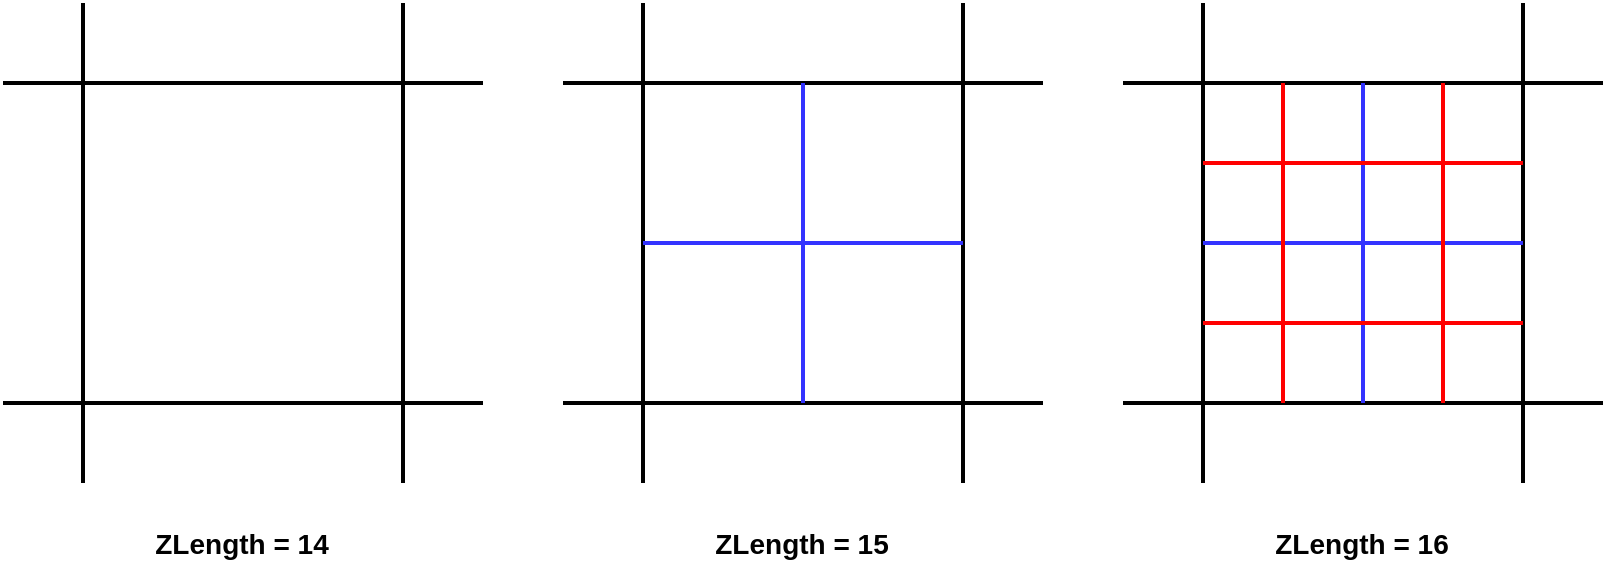
\includegraphics[width=\linewidth]{images/zlength.png}
    \caption{Zones as Perceived by Node of Different ZLengths}
    \label{fig:zlength}
\end{figure}

The zone agent connects to a GPS device using a Unix socket, and uses it to continuously read the node's latitude and longitude. The latitude and longitude are mapped from degrees to 16-bit integers to calculate the x and y coordinates. Afterward, the ZLength most significant bits of the coordinates are concatenated to form the \acrfull{zid}. If the zone agent detects that the zone is changed, it informs other submodules (subscribers) to take appropriate actions according to their logic.

\begin{figure}[!htb]
    \centering
    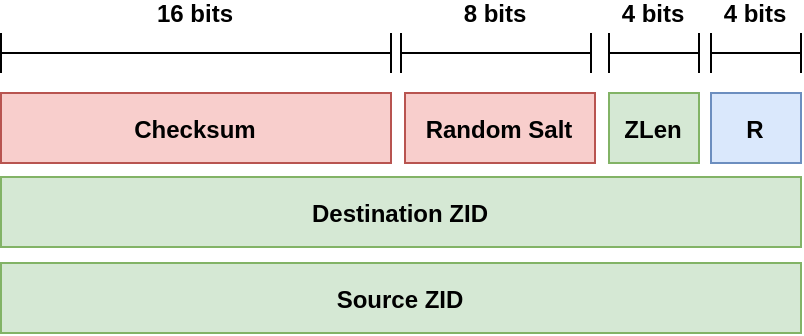
\includegraphics[width=0.8\linewidth]{images/zid.png}
    \caption{\acrshort{zid} Header}
    \label{fig:zid}
\end{figure}

The zone agent keeps track of the current zone of the node for other submodules to use. It also provides some utilities to calculate distances between zones, check if two zones are intersecting (as they may have different ZLengths), check if two zones are exactly the same, and calculate the area of a zone (which is used by Variable Radius Broadcasting). Since it holds the information of the node's current zone, other submodules use it to create \textbf{\acrshort{zid} Headers}. In our implementation of \acrshort{zhls}, a \acrshort{zid} Header is prepended to most control and data packets. It contains information about the source and destination zones, as shown by Figure \ref{fig:zid}. The header fields are as follows:
\begin{itemize}[itemsep=1pt, topsep=5pt]
    \item \textbf{ZLen:} The ZLength of the Source \acrshort{zid} and Destination \acrshort{zid} fields.
    \item \textbf{Destination \acrshort{zid}:} The Zone ID of the destination.
    \item \textbf{Source \acrshort{zid}:} The Zone ID of the source.
    \item \textbf{Random Salt:} Randomly added bits so that the encryption of a \acrshort{zid} header with the same source and destination nodes varies.
    \item \textbf{Checksum:} A checksum of the previous fields used to validate the \acrshort{zid} header.
\end{itemize}

\subsubsection{Secure \acrshort{arp}}
\qquad \acrfull{arp} is a protocol used in \acrshort{ip} networks to map layer-3 \acrshort{ip} addresses to layer-2 \acrshort{mac} addresses. \acrshort{arp} is vulnerable to \acrshort{mac} spoofing attacks, where someone in the network masquerades as someone else. Since \acrshort{caian} has many use cases where communications security is critical, we decided not to use the \acrshort{arp} protocol implementation in Linux. Instead, we implemented a secure version that we call Secure \acrshort{arp}.

Secure \acrshort{arp} is a simple protocol, similar to \acrshort{arp}, that is used in our system for three reasons:
\begin{itemize}[itemsep=1pt, topsep=5pt]
    \item Identify the direct neighbor hosts (or neighbor zones) of any given host.
    \item Find the \acrshort{ip} address to \acrshort{mac} address mapping for those direct neighbors.
    \item Calculate the latency for communicating with each neighbor node.
\end{itemize}
The main reason that Secure \acrshort{arp} can use encryption to secure its communications while \acrshort{arp} cannot, is that all nodes in a tactical team network can easily share a secret key. This is not the case in any \acrshort{ip} network, where the users may have no idea who else is present on the same network.

\begin{figure}[!htb]
    \centering
    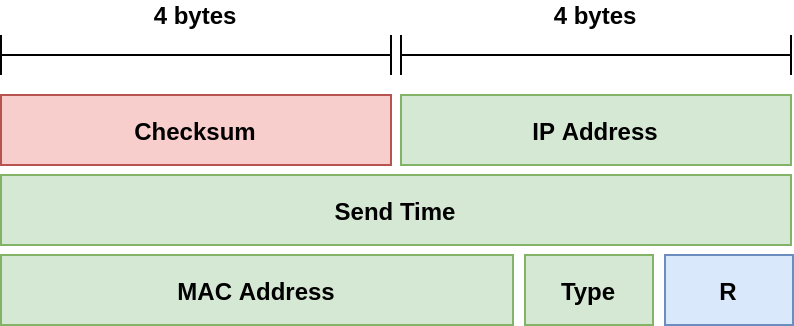
\includegraphics[width=0.8\linewidth]{images/sarp_header.png}
    \caption{\acrshort{sarp} Header}
    \label{fig:sarp-header}
\end{figure}
In Secure \acrshort{arp}, all packets consist of a \acrshort{zid} header and a \acrshort{sarp} header that is shown by Figure \ref{fig:sarp-header}. The header fields are as follows:
\begin{itemize}[itemsep=1pt, topsep=5pt]
    \item \textbf{Type:} \acrshort{sarp} packets are either a \textit{\acrshort{sarp} Request} or a \textit{\acrshort{sarp} Response}.
    \item \textbf{\acrshort{ip} address:} The \acrshort{ip} address of the sender.
    \item \textbf{\acrshort{mac} address:} The \acrshort{mac} address of the sender.
    \item \textbf{Send Time:} The time at which the packet was sent.
    \item \textbf{Checksum:} A checksum of the previous fields used to validate the \acrshort{sarp} header.
\end{itemize}

\begin{figure}[!htb]
    \centering
    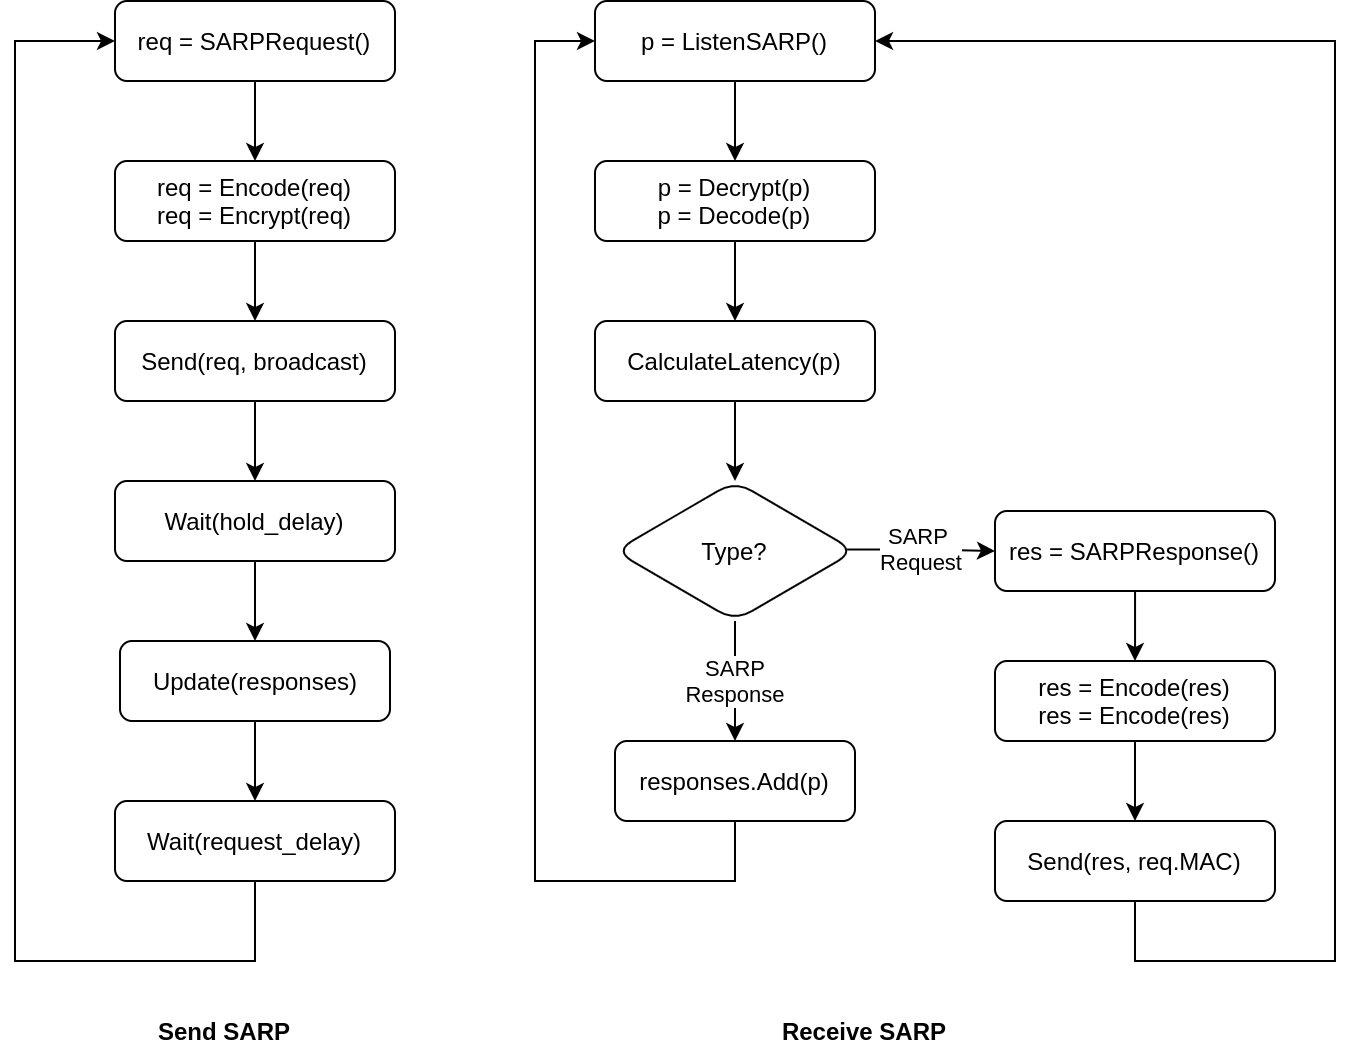
\includegraphics[width=\linewidth]{images/sarp_flowchart.png}
    \caption{\acrshort{sarp} Protocol}
    \label{fig:sarp-flowchart}
\end{figure}

\acrshort{sarp} operates through the two concurrent routines \textit{Send \acrshort{sarp}} and \textit{Receive \acrshort{sarp}} shown by Figure \ref{fig:sarp-flowchart}.
Some details are omitted for conciseness. For example, when a \acrshort{sarp} packet is received, it is actually processed in a different routine than the listening one to avoid missing a \acrshort{sarp} packet while processing a previous one.

The \acrshort{sarp} protocol operates by periodically sending and receiving \acrshort{sarp} requests and responses to find the node's direct neighbors and their information. It maintains a \textit{Neighbors Table} that contains the Node ID (\acrshort{ip} or Zone ID), \acrshort{mac} address, and most up-to-date latency of each direct neighbor node or zone. When a neighbor belongs to a different zone, it is considered as a neighbor zone rather than a neighbor node. This is determined by the \acrshort{zid} header. The \textit{Neighbors Table} is used by the Unicast Controller, as will be shown later in this chapter.

The \textit{Send \acrshort{sarp}} routine starts by creating an \acrshort{sarp} Request, encoding it into binary, and encrypting it. Afterwards, it sends the packet through the \acrshort{mac} layer to all nodes within range. The routine then waits for a hold period, giving a chance for neighbors to respond. The responses collected by the \textit{Receive \acrshort{sarp} routine} are used to update the Neighbors Table. The routine then waits again for an inter-request delay before sending the next request. The \textit{Send \acrshort{sarp}} routine also detects whether the neighbors have changed between subsequent requests by comparing hashes of the Node IDs in the Neighbors Table before and after it collects responses.

The \textit{Receive \acrshort{sarp}} routine continuously listens for \acrshort{sarp} packets. When a packet is received, it is decrypted and decoded. The latency between the current node and the sender is then calculated. If the received packet is an \acrshort{sarp} response, it is collected for the operation of the \textit{Send \acrshort{sarp}} routine. Otherwise, if is an \acrshort{sarp} Request, a response is created, encoded, encrypted, and sent through the \acrshort{mac} layer to the sender.

One last missing detail is how \textit{CalculateLatency} procedure calculates the latency information between the current node and the sender node using the send time in the \acrshort{sarp} header. To calculate the latency accurately, both nodes must be in sync. Since most tactical devices have a GPS, we assume that the GPS is used for time synchronization. 


\subsubsection{Hierarchical LSR}

\qquad Hierarchical Link State Routing (LSR) is the method through which nodes exchange information about the network. It is based on Link State Routing (LSR), in which every node constructs a connectivity graph of the whole network. However, in \acrshort{zhls} every node only maintains information about the nodes inside its own zone, in addition to zone connectivity information. It consists of two main components: Intrazone LSR and Interzone LSR.

\begin{figure}[!htb]
    \centering
    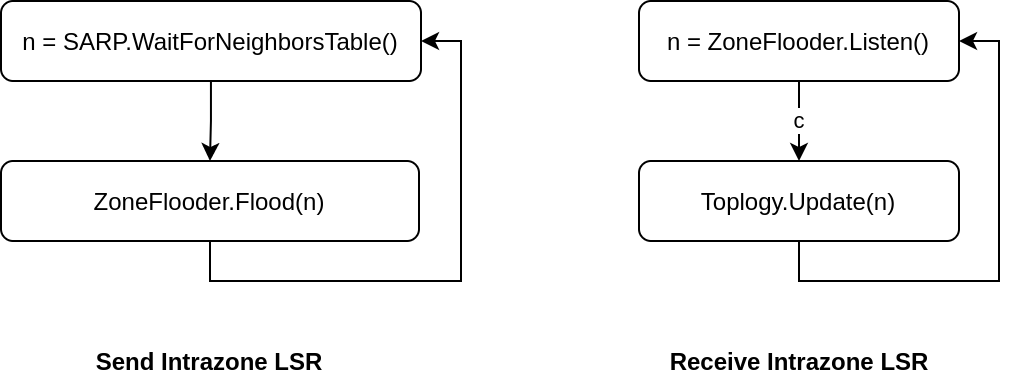
\includegraphics[width=\linewidth]{images/lsr_flowchart-intrazone.png}
    \caption{Intrazone LSR}
    \label{fig:intrazone-lsr}
\end{figure} 

In Intrazone LSR, a zone flooder is used to flood the Neighbors Table produced by Secure \acrshort{arp} every time it is updated. All nodes in a zone receive Intrazone LSR updates periodically from each other and compute connectivity information about all nodes in the zone, and the connectivity of their zone to its direct neighbor zones. Intrazone LSR is illustrated by the \textit{Send Intrazone LSR} and \textit{Receive Intrazone LSR} concurrent routines shown by Figure \ref{fig:intrazone-lsr}.

\begin{figure}[!htb]
    \centering
    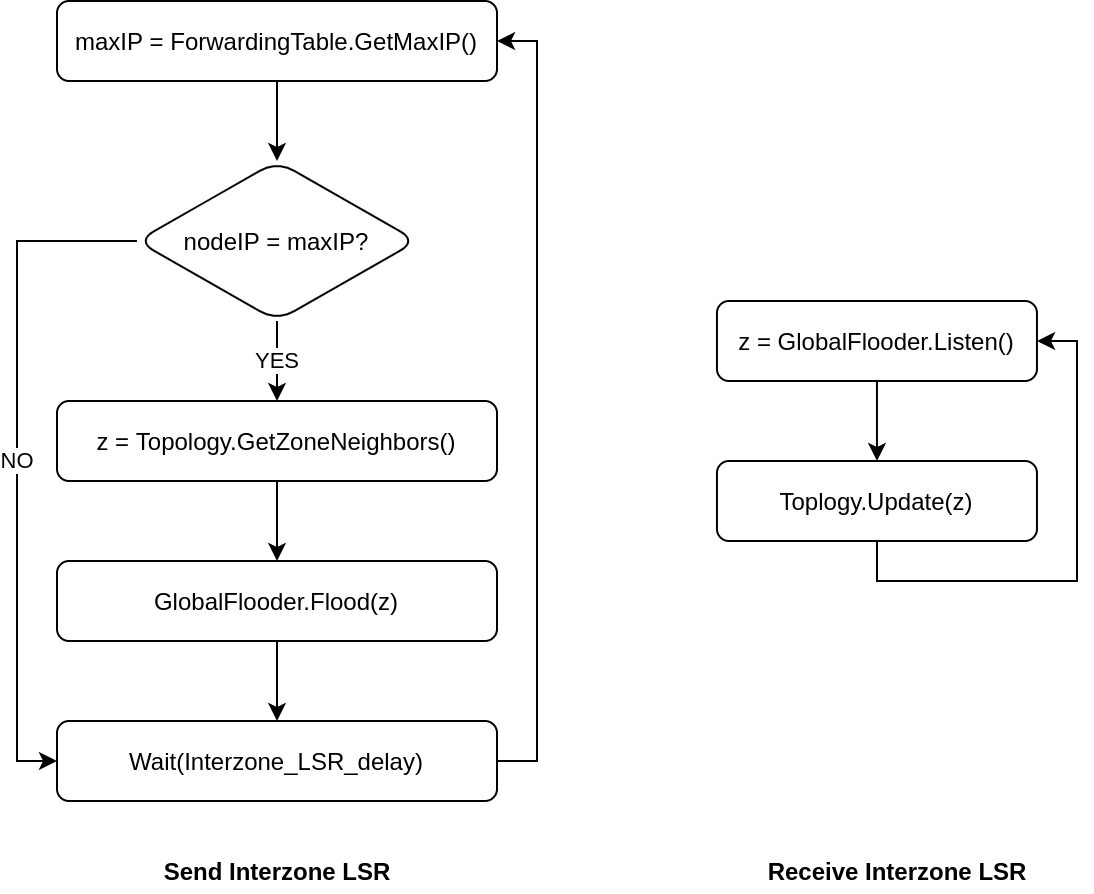
\includegraphics[width=\linewidth]{images/lsr_flowchart-interzone.png}
    \caption{Interzone LSR}
    \label{fig:interzone-lsr}
\end{figure}

In Interzone LSR, a global flooder is used to flood a special Zone Neighbors Table to all the nodes in the network periodically. A Zone Neighbors Table of a zone contains the zones that it has direct connectivity to. All nodes in the network receive Interzone LSR updates from all zones and compute connectivity information about all zones.  Interzone LSR is illustrated by the \textit{Send Interzone LSR} and \textit{Receive Interzone LSR} concurrent routines shown by Figure \ref{fig:interzone-lsr}.

A question that naturally rises in Interzone LSR is which node is responsible for sending Interzone LSR in each zone. In the original \acrshort{zhls} paper, all nodes flood Interzone LSR packets. However, this incurs a huge bandwidth overhead. In our implementation, we designed a simple scheme to avoid this. Since all nodes in a zone know the \acrshort{ip} addresses of each other (through Secure \acrshort{arp} and Intrazone LSR), they can all agree on which node has the highest \acrshort{ip} address. Hence, all nodes in a zone delegate the task of flooding Interzone LSR packets to the node with the highest \acrshort{ip} address. One might argue that with mobility and packet loss, nodes may disagree on which node has the highest \acrshort{ip} address, causing multiple ones to send Interzone LSR packets. Even though this case might occur only temporary, having two or three nodes flooding Interzone LSR packets is still better than having all the nodes in the zone do it.


\subsubsection{Hierarchical Topology Graph}
\qquad The topology graph is a major component of any proactive or hybrid routing protocol that is used to keep up-to-date routing information and is used to compute the best path from some source (usually the router itself) to any reachable destination. \acrfull{zhls} is divided into two topologies: node-level and zone-level. Consider the case when you require a path to a distant location (Interzone routing). The source node must consider both node-level and zone-level topologies and use the shortest route method on both. Aside from the memory requirements for both topologies. So we reasoned that merging both topologies into a single one with distinct types of nodes would be more efficient.\\ \\
Topology graph in \acrshort{caian} has two different type of vertices, nodes and zones as show in Figure \ref{fig:topology}. Node vertices (represented by circles) represent nodes that exist in the same zone with the router itself and each one is identified by the node \acrshort{ip}, while zone vertices (represented by squares) represent zones that are reachable from that router and each one is identified by the zone ID. 

\begin{figure}[!htb]
    \centering
    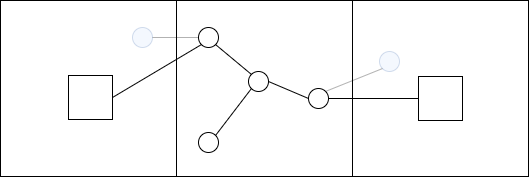
\includegraphics[width=\linewidth]{images/topology.png}
    \caption{Hierarchical Topology Graph}
    \label{fig:topology}
\end{figure} 
The following two approaches are used to keep the topology graph up-to-date for all nodes and zones routing information:
\begin{itemize}[itemsep=1pt, topsep=5pt]
    \item Periodically receives Intrazone and Interzone LSR packets as illustrated previously and uses this information to update the topology graph vertices, edges, and weights.
    \item Each vertex in the graph should have a timer attached to it (nodes and zones). Once we have received an LSR packet from that vertex, reset the timer (Intrazone LSR packets for node vertices and Interzone LSR packets for zone vertices). Remove this vertex from the topology graph instantly once the timer goes off.\\
\end{itemize} 
Keeping the topology graph up-to-date is mandatory as it will be used mainly for two important functionalities: 
\begin{itemize}[itemsep=1pt, topsep=5pt]
    \item Find the shortest paths by applying the Dijkstra algorithm (using latency metric) to all nodes and zones in the graph and use this information to fill the forwarding table.
    \item Find all reachable neighbor zones by applying controlled depth-first search from the router vertex till reaching zone vertices and use this information to apply zone-level broadcasting, which is much more efficient than normal flooding.
\end{itemize}

\subsubsection{Destination Zone Discovery}
Destination Zone Discovery (DZD) is a major module in  \acrfull{zhls}. Consider the case when the source node require a path to a node that is outside its zone (Interzone routing). The first step is to discover the zone of the required destination. 

Destination Zone Discovery (DZD) protocol has two types of control messages that control the searching process: DZD Request which is sent using zone-level broadcasting by the router that want to discover the destination zone and DZD Response which is sent using normal unicasting from the node that know the destination zone to the source node which its zone was already stored in the DZD Request header. 

DZD Request control message must contain two headers: 
\acrshort{zid} header which has the following fields:
\begin{itemize}[itemsep=1pt, topsep=5pt]
    \item \textbf{Src Zone:} The zone ID of the source node which will be used later to send the DZD Response to.
    \item \textbf{Dst Zone:} The zone ID of the neighbor zone to the source zone which is the DZD Request will be sent to.
\end{itemize} 

And DZD Request Header which has the following fields as show in Figure \ref{fig:dzd-request}:
\begin{itemize}[itemsep=1pt, topsep=5pt]
    \item \textbf{Src \acrshort{ip}:} The \acrshort{ip} of the source node which will be used later to send the DZD Response to.
    \item \textbf{Required Dst \acrshort{ip}:} The \acrshort{ip} of the destination node which it's required to know its zone.
    \item \textbf{Visited Zones:} Array of all zones that the DZD Request message has already gone through. This array is used to prevent recirculation of the same message indefinitely. 
\end{itemize} 

\begin{figure}[!htb]
    \centering
    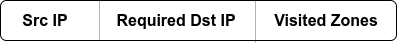
\includegraphics[scale=0.7]{images/dzdrequest_header.png}
    \caption{DZD Request Header}
    \label{fig:dzd-request}
\end{figure} 

The reachable neighbor zones are found using depth-first search on the hierarchical topology graph, and a copy of the DZD Request message is sent to each of them once the DZD Request message is generated using the preceding headers. Each zone will repeat the process until the destination zone is discovered.

The first node that receive the DZD Request message at the destination zone will stop broadcasting DZD Request message and start to form DZDResponse message using \acrshort{zid} header which contains:
\begin{itemize}[itemsep=1pt, topsep=5pt]
    \item \textbf{Dst Zone:} The zone ID of the destination zone which, in this case, the zone of the source node that started broadcasting DZD Response message.
\end{itemize} 

And DZD Response Header which has the following fields as show in Figure \ref{fig:dzd-response}: 
\begin{itemize}[itemsep=1pt, topsep=5pt]
    \item \textbf{Dst \acrshort{ip}:} The \acrshort{ip} of the destination node which, in this case, the source node that started broadcasting DZD Response message.
    \item \textbf{Required Dst \acrshort{ip}:} The \acrshort{ip} of the destination node which it's required to know its zone.
    \item \textbf{Required Dst Zone ID:} The destination zone ID which the source node was looking for it.
\end{itemize} 

\begin{figure}[!htb]
    \centering
    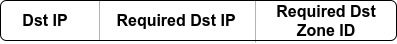
\includegraphics[scale=0.7]{images/dzdresponse_header.png}
    \caption{DZD Response Header}
    \label{fig:dzd-response}
\end{figure} 

Using the Dst \acrshort{ip} in DZD Response Header and Dst Zone in \acrshort{zid} Header, DZD Respone packet can be unicasted to the original source that sent DZD Request message. Each node along the path of DZD Respone and the original source itself cache the destination zone for upcoming messages.

The original source can transmit all data buffered to that destination after receiving the DZD Response message. If the search fails, it will be repeated three times, each time after a certain amount of time, until the target zone is found, otherwise it will be announced as a failure and all stored packets for that destination will be discarded.

\section{Multicast Controller}
\subsection{Functional Description}
The multicast controller is in charge of many-to-many transmission between network nodes; that is, multiple senders and multiple receivers, each with an \acrshort{ip} address. At every node, it creates a Multi-Forwarding table, which includes the best next-hops to forward a packet to for each possible multicast group. Collectively, this constitutes by periodically sending control packets join query and join replies and filling tables in every. As indicated in the preceding section, we believe On-Demand Multicast Routing Protocol (ODMRP) is one of the best multicast protocols for this task. As a result, we chose it to be our multicast routing protocol.

\subsection{Modular Decomposition}

\begin{figure}[!htbp]
    \centering
    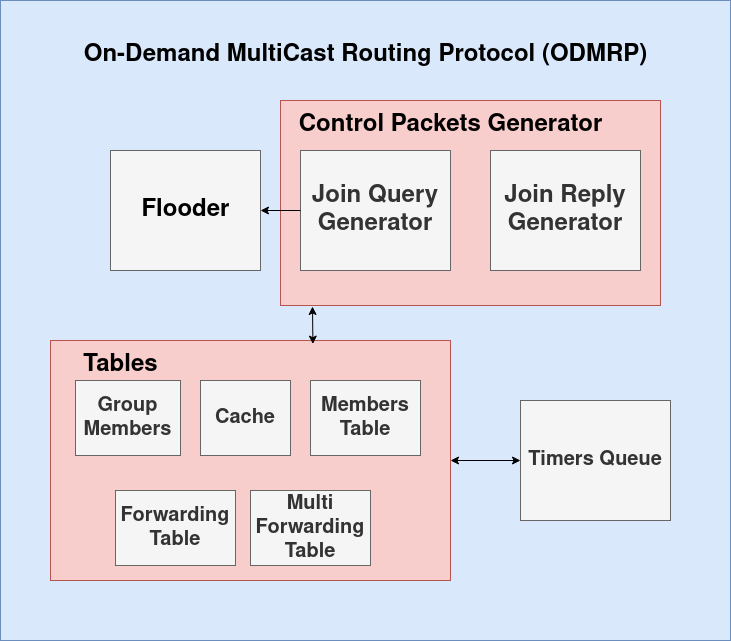
\includegraphics[width=\linewidth]{images/odmrp-modules.png}
    \caption{ODMRP Modules}
    \label{fig:odmrp-modules}
\end{figure}

On-Demand Multicast Routing Protocol (ODMRP) may be divided into two part, the control packet generator and the tables. In addition, there is a flooder module is in charge of flooding the join query packets and timers queue for deleting expired table entries from the tables. ODMRP modules can be show in Figure  \ref{fig:odmrp-modules}
\\
\subsubsection{Control Packets Generator}
Generating right control packets is critical for this protocol as ODMRP depends on the control packets for filling the tables, construct the routes and the network soft state maintenance.
This module generates two important control packets called Join Query (format illustrated in Figure \ref{fig:join-query}) and Join Reply (format illustrated in Figure \ref{fig:join-reply}).
\\
A Join Query is generated when a multicast source has packets to transmit but no route and group membership is known, a Join Query packet contains the following fields: 
\begin{itemize}[itemsep=1pt, topsep=5pt]
    \item \textbf{Dests Count:} The Number of destinations IPs.
    \item \textbf{Checksum:} It is used to validate the received control packet.
    \item \textbf{SeqNo:} Unique sequence number of the control packet.
    \item \textbf{TTL:} Time to live, which is the number of hops this packet can traverse.
    \item \textbf{SrcIP:} Source \acrshort{ip} address where the control packet is generated.
    \item \textbf{GrpIP:} Group \acrshort{ip} address of this multicast group.
    \item \textbf{PrevHop:} Mac address of the last node which has processed this packet.
    \item \textbf{DestIPs:} The destination IPs of this multicast group.
\end{itemize} 

\begin{figure}[!htbp]
    \centering
    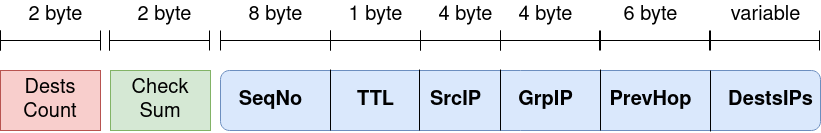
\includegraphics[width=\linewidth]{images/join-query.png}
    \caption{Join Query Packet}
    \label{fig:join-query}
\end{figure}

Join Query control packet is generated using the following:
\begin{itemize}[itemsep=1pt, topsep=5pt]
    \item \textbf{SeqNo:} Incremental value in the multicast control module,
    different for each control packet sent.
    \item \textbf{TTL:} Default time to live value in our case we set it to 100.
    \item \textbf{SrcIP:} This Node \acrshort{ip} where the join query packet is generated.
    \item \textbf{GrpIP:} Group \acrshort{ip} address of this multicast group.
    \item \textbf{PrevHop:} \acrshort{mac} of current node.
    \item \textbf{DestIPs:} The destination IPs of this multicast group \acrshort{ip}.
\end{itemize}

Then this Join Query packet is flooded using the flooder and gets updated and update the node's tables until it reaches a destination the destination node generates a Join Reply control packet which contains the following fields:
\begin{itemize}[itemsep=1pt, topsep=5pt]
    \item \textbf{Next Hops Count:} Next Hops \acrshort{mac} addresses count which equals the source IPs address count either.
    \item \textbf{Checksum:} It is used to validate the received control packet.
    \item \textbf{SeqNo:} Unique sequence number of the control packet.
    \item \textbf{DestIP:} Destination \acrshort{ip} where the Join Reply is generated.
    \item \textbf{GrpIP:} Group \acrshort{ip} address of this multicast group.
    \item \textbf{PrevHop:} Mac address of the last node which has processed this packet.
    \item \textbf{SrcIPs:} Source IPs addresses where the control packet is generated.
    \item \textbf{Next Hops:} Next Hops \acrshort{mac} addresses to reach the sources.
    \item \textbf{Cost:} Cost of this path, which equals the number of hops.
\end{itemize}

\begin{figure}[!htbp]
    \centering
    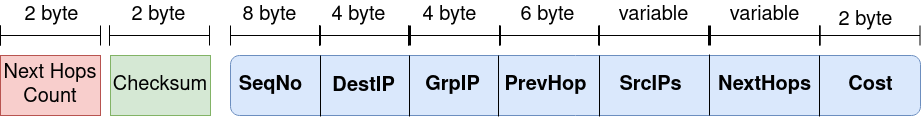
\includegraphics[width=\linewidth]{images/join-reply.png}
    \caption{Join Reply Packet}
    \label{fig:join-reply}
\end{figure}

Join Reply control packet is \textbf{generated} using the following:
\begin{itemize}[itemsep=1pt, topsep=5pt]
    \item \textbf{SeqNo:} Received join query sequence number.
    \item \textbf{DestIP:} \acrshort{ip} of the current node where the Join Reply is generated.
    \item \textbf{GrpIP:} Group \acrshort{ip} address of this multicast group.
    \item \textbf{PrevHop:} Mac address of the current node.
    \item \textbf{SrcIPs:} Filled using cache table by iterating on cache table entries and checks if the group \acrshort{ip} is equal to the group IP of this multicast group, if true it appends the source IP found in the cache table to this join reply control packet.
    \item \textbf{Next Hops:} Filled using cache table by iterating on cache table entries and checks if the group \acrshort{ip} is equal to the group IP of this multicast group, if true it appends the next hop found in the cache table to this join reply control packet.
    \item \textbf{Cost:} 1.
\end{itemize}

Then Join Reply packet is sent to the next hops addresses and gets updated and update the tables then passed to the next hops addresses until it reaches the multicast sources.

\subsubsection{Tables}
As we knew in Chapter \ref{ch:literature-survey} ODMRP are mesh based and soft state protocol, so tables play big role in ODMRP protocol to construct the mesh, forwarding group members and the routes to reach the destinations nodes.

\textbf{Group Members Table} is the table which is used to hold the multicast group \acrshort{ip} address and the corresponding destinations \acrshort{ip} addresses So a packet can be sent using only the group \acrshort{ip}, Figure \ref{fig:group-members-table-entry} represents one entry of Group Members Table, It is filled by a configuration file in the senders nodes.
\begin{figure}[!htbp]
    \centering
    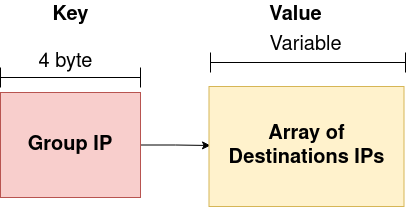
\includegraphics[scale=0.7]{images/group-members-table-entry.png}
    \caption{Group Members Table}
    \label{fig:group-members-table-entry}
\end{figure}
\\
\\
\textbf{Cache Table} is the table that holds the control packet source \acrshort{ip} and the corresponding (Sequence Number, Group \acrshort{ip}, Previous Hop and cost). And the table is used to:
\begin{enumerate}
    \item Check for control packet duplicates.
    \item Hold cost value to check if a better entry has been found.
    \item Generate and update join reply control packet.
\end{enumerate}
Figure \ref{fig:cache-table-entry} represents one entry of Cache Table.
\begin{figure}[!htbp]
    \centering
    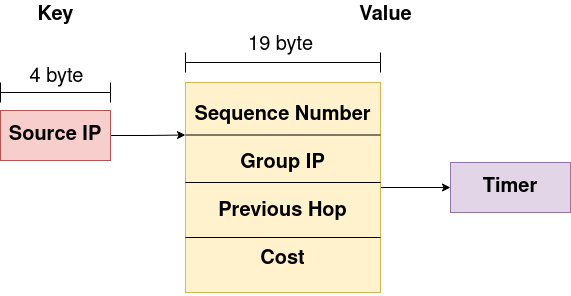
\includegraphics[width=\linewidth]{images/cache-table-entry.png}
    \caption{Cache Table Entry}
    \label{fig:cache-table-entry}
\end{figure}
\\
\\
\textbf{Members Table} is a table that holds the group IPs that the current node is a part of. This table for faster checking that the current node is a destination of a certain multicast group \acrshort{ip} address, and it gets filled the first time the node knew it is a destination of a certain multicast group \acrshort{ip} address. Figure \ref{fig:member-table-entry} represents one entry of Members Table.
\begin{figure}[!htbp]
    \centering
    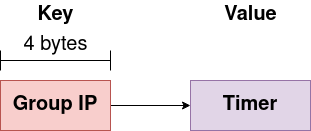
\includegraphics[scale=0.8]{images/member-table-entry.png}
    \caption{Members Table Entry}
    \label{fig:member-table-entry}
\end{figure}
\\
\\
\textbf{Forwarding Table} is a table that holds some entries, each one has a destination \acrshort{ip} address and the corresponding next hop \acrshort{mac} address and cost. It gets filled when receiving a join reply from a destination, and it is used to update the Multi Forward Table (more details in the next section \ref{sec:odmrp-protocol-flow}).
Figure \ref{fig:forwarding-table-entry} represents one entry of Forwarding Table.

\begin{figure}[!htbp]
    \centering
    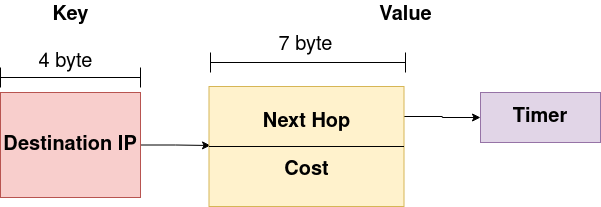
\includegraphics[width=\linewidth]{images/forwarding-table-entry.png}
    \caption{Forwarding Table Entry}
    \label{fig:forwarding-table-entry}
\end{figure}

\textbf{Multi Forward Table} is a table that holds some entries, each one has a multicast group \acrshort{ip} address and the set of corresponding next hops to reach this multicast group \acrshort{ip} destinations. It gets filled when receiving a join reply from a destination (more details in the next section \ref{sec:odmrp-protocol-flow}), and this table is used by the node router to direct the packets to reach destinations node of a certain multicast group \acrshort{ip} address.
Figure \ref{fig:multi-forward-table-entry} represents one entry of Multi Forward Table.
\begin{figure}[!htbp]
    \centering
    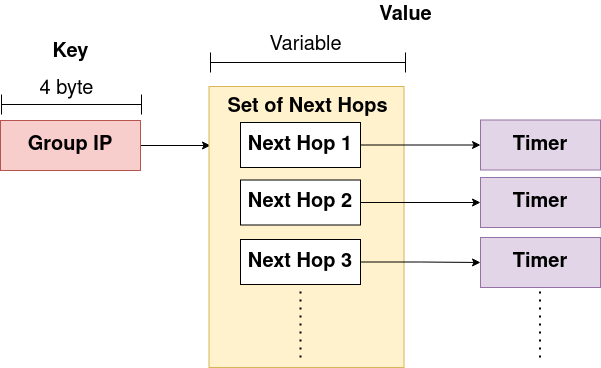
\includegraphics[width=\linewidth]{images/multi-forward-table-entry.png}
    \caption{Multi Forward Table Entry}
    \label{fig:multi-forward-table-entry}
\end{figure}
\\
\\
\\
\\
\\
\\
\subsection{ODMRP Protocol Flow}
\label{sec:odmrp-protocol-flow}
In ODMRP \cite{ODMRP}, group membership and multicast routes are formed and updated by the source on demand. When a multicast source has packets to transmit but no route and group membership is known (Multi Forward \ref{fig:multi-forward-table-entry} Table is empty), it floods an advertising control packet. This packet, named Join Query (format illustrated in Figure \ref{fig:join-query}) and it is regularly sent by the flooder to the whole network to refresh the membership information and update the routes.
\\
\\
When a node gets a Join Query packet, time to live is decreased by one, and it records the source address and the unique identifier of this control packet to its Cache Table \ref{fig:cache-table-entry} to identify duplication to construct the join reply later.
If the Join Query control packet is not a duplicate by verifying it is not a duplicate from the cache table and the Time to live is higher than zero, the cache table is updated, and it is rebroadcast.
\\
\\
When a Join Query packet reaches the multicast receiver, it adds the group \acrshort{ip} to its member table as an entry (Figure \ref{fig:member-table-entry}) so the node realizes that it is a part of this forwarding  group with a specific group \acrshort{ip} address.
\\
The destination node then generates a Join Reply control packet (format shown in Figure \ref{fig:join-reply}) with the help of the cache table to add next hops and source IPs which are filled before by the received join queries and sets the cost of the generated join reply to be one.
\\
\\
Then sends the generated join reply to the previous hops nodes, The classical ODMRP protocol floods the join replies packet until it reaches all the sources, We did an \textbf{optimization} by sending the join reply via the next hops stored in the cache and making the join reply propagated and received by only the forwarding group members and not broadcasted to any other node which are not a part of this multicast group.
\\
After generating the join reply control packet sends the join reply with the same manner by updating the source IPs, next hops, the cost, update the forwarding table \ref{fig:forwarding-table-entry} and also construct the routes by filling the multi forward table \ref{fig:multi-forward-table-entry} with the next hops \acrshort{mac} addresses corresponding to this group \acrshort{ip} address.
Updating the route in the Multi Forward Table is done by checking if the forwarding table is updated by a newly added destination \acrshort{ip} or destination \acrshort{ip} address exists but the new received join reply cost is less than the existing one. If this is true, both the forwarding table and multi forward table are updated by adding the previous hop of the received join reply to the Next hops set, using the group \acrshort{ip} as the key of the next hops.
\\
\\
This method generates a mesh of nodes with forwarding group members and routes from sources to receivers until it reaches the multicast source through chosen paths.
\\
When the node's router wants to send a multicast packet is checks if Multi Forward Table has entries using this multicast group \acrshort{ip} address as the key, and it can access a set of next hops to send the packet to them, so it can do multicasting.

\section{Command Center Client}
Command centers are responsible for the central administration and operational management of a group of units. High-end computers with strong CPUs, high power consumption capabilities, and large storage and RAM capabilities are expected to be used as command center clients. The command centers are located near the operation field and have a wide wireless range, allowing them to link to a group of troops in the field. They're assumed to have limited (or no) mobility.


\subsection{Functional Description}
Command centers in \acrshort{caian} have the ability to collect data from a collection of units, show it to the operators or unis leaders, and control these units by delivering a series of instructions.
What exactly a command center can perform is summarized briefly in the following list:
\begin{itemize}[itemsep=1pt, topsep=5pt]
\item Send audio command and command codes to a single unit.
\item Send audio commands to a group (multicast) or everyone (unlimited-radius broadcast).
\item Store all sent and received data.
\item Show old data (audio, messages, videos, sensor data)
\item Show notifications when an audio message or command code is received.
\item Show video streams as they are received from units.
\item Show a map of connected units distinguished by group color to each unit belonging to some group.
\item If sensor data isn’t received in 2 minutes, mark the unit as inactive and notify the command center operators.
\item  If a unit’s heartbeat is below a threshold, mark it as in danger and notify the command center operators.
\end{itemize} 

\subsection{Modular Decomposition}
As illustrated in Figure \ref{fig:cmd-center}, \acrshort{caian}'s command center is organized into two major modules: Daemon, which is in charge of sending and receiving data from other units in the network, and User Interface, which allows operation leaders to manage and visualize this data as well as record command audios and choose command codes that they want to send to these units.

\begin{figure}[!htb]
    \centering
    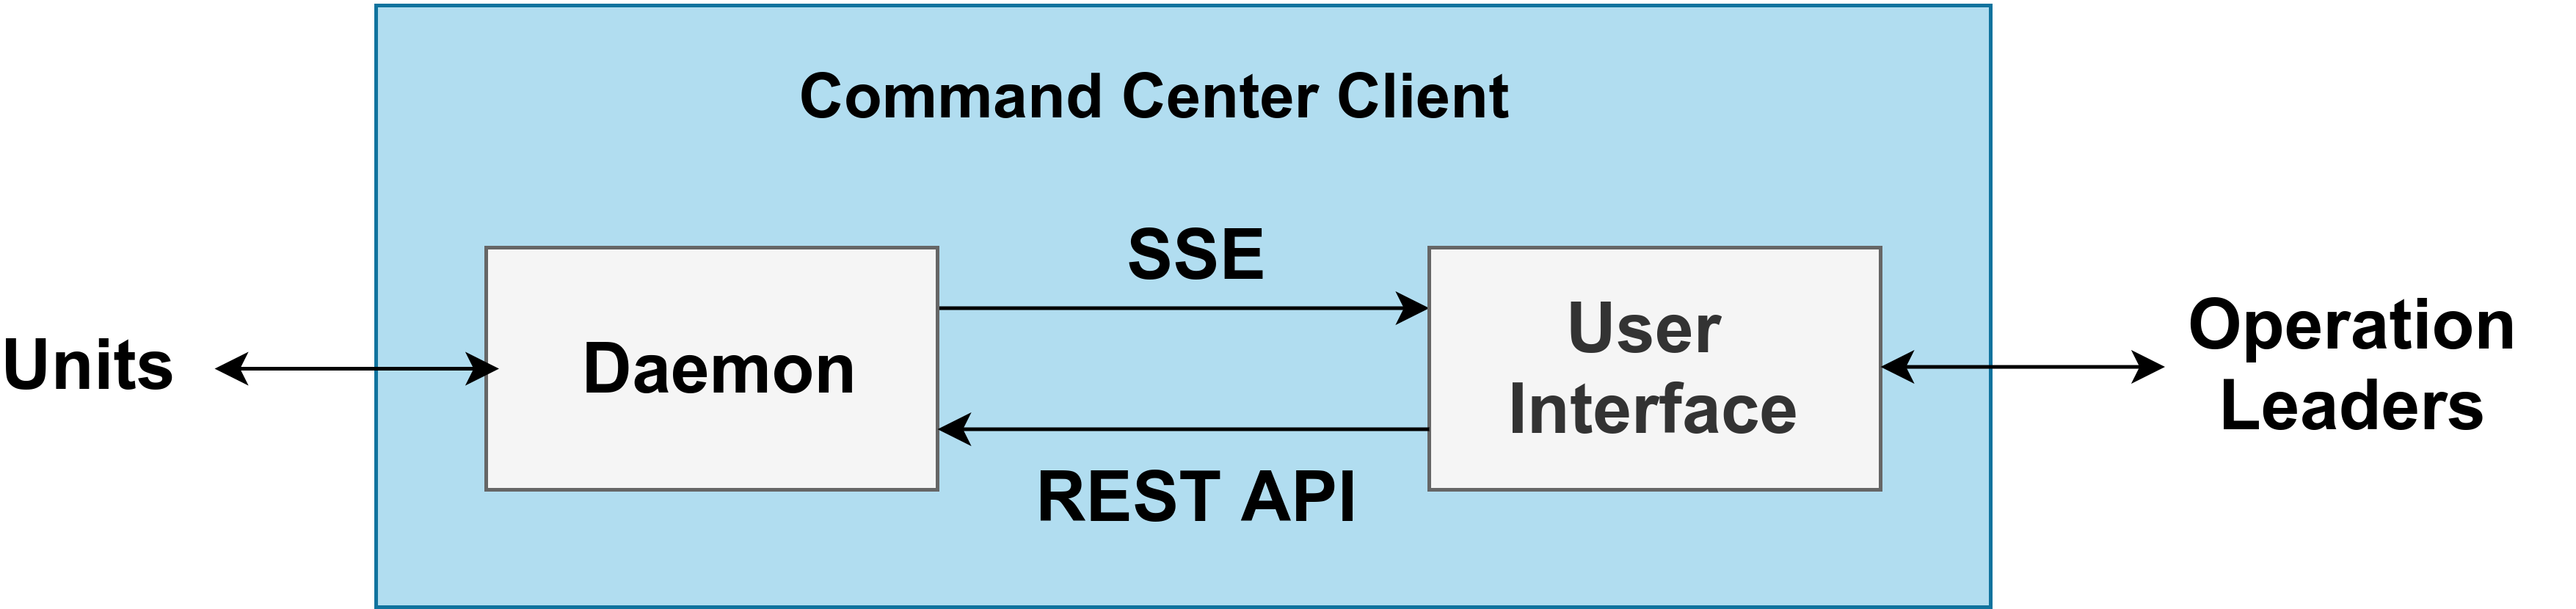
\includegraphics[width=\linewidth]{images/command-center.png}
    \caption{Command Center Client}
    \label{fig:cmd-center}
\end{figure}

Video Streamer is a submodule of both the Daemon and User Interface that will be discussed in better detail later.

\subsubsection{Daemon}
The daemon of the command center client is a highly concurrent program that runs in the background on the command center's devices. It exchanges code messages, audio messages with units, and receive sensors data and video streaming from the units through a network interface, runs a database to keep track of all sent and received data, and connects to the user interface through a \acrshort{rest}ful \acrshort{api} server.

On the network interface, the unit has two concurrent routines that listen for TCP connections and UDP datagrams. When receiving a TCP connection or a UDP datagram, the incoming data is handled in a separate concurrent routine to avoid missing connections or incoming datagrams while processing previous ones. Any data received is prepended with a byte that identifies the packet type. The packet payload is then decoded, the data is stored in the database, and the user interface is notified through \acrfull{sse}. The network interface also provides routines to send or receive packets over TCP or UDP to units, in case the command center needs to send code messages or audio messages to a unit, a group of units, or all the units. Note that all TCP and UDP data transfers are routed using our router.

The \acrshort{rest}ful \acrshort{api} server runs in a concurrent routine and provides endpoints for the user interface to collect and present stored data. In addition, it provides endpoints for the user interface to send code messages or audio messages to unit(s). All sent and received data are stored in the database. Since the database is accessed through different concurrent subroutines, mutual exclusion techniques are used to synchronize access to the database.

The main routine reads any necessary configuration or command line arguments on startup, initializes the database, then starts and orchestrates the aforementioned subroutines. Figure \ref{fig:cmd-daemon} shows a complete picture of the command center client daemon.

\begin{figure}[!htb]
    \centering
    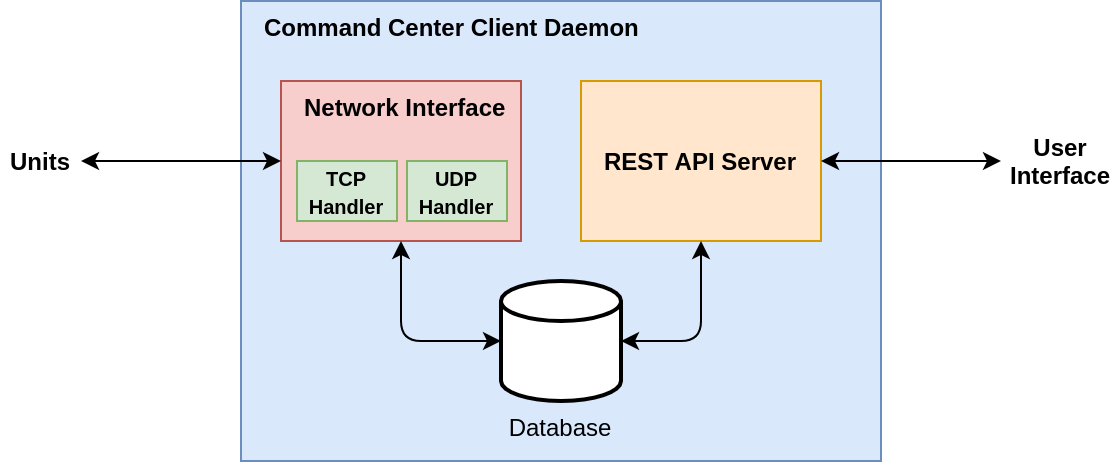
\includegraphics[width=\linewidth]{images/cmd-daemon.png}
    \caption{Command Center Client Daemon}
    \label{fig:cmd-daemon}
\end{figure} 

\subsubsection{Video Streamer}
For video streaming, we use HTTP Live Streaming (HLS) protocol. While video streaming is running at a unit, the command center client receives a metadata file and video segment files from the units continuously. The video streamer receives those files through the daemon, continuously updates the metadata, and stores the video segment files. In a dedicated media directory, the video streamer creates a directory per video stream per unit to store the video stream's metadata and video segment files and serve them to the user interface through a file server \acrshort{api} which maps endpoints paths to local file system paths.

When a video stream starts, the video streamer notifies the user interface through a \acrshort{sse}. The user interface reads the metadata to identify the available video segments, and starts fetching the video segments and displaying the video stream continuously through the file server \acrshort{api}. Figure \ref{fig:video-streamer} visualizes the data flow through the video streamer.

\begin{figure}[!htb]
    \centering
    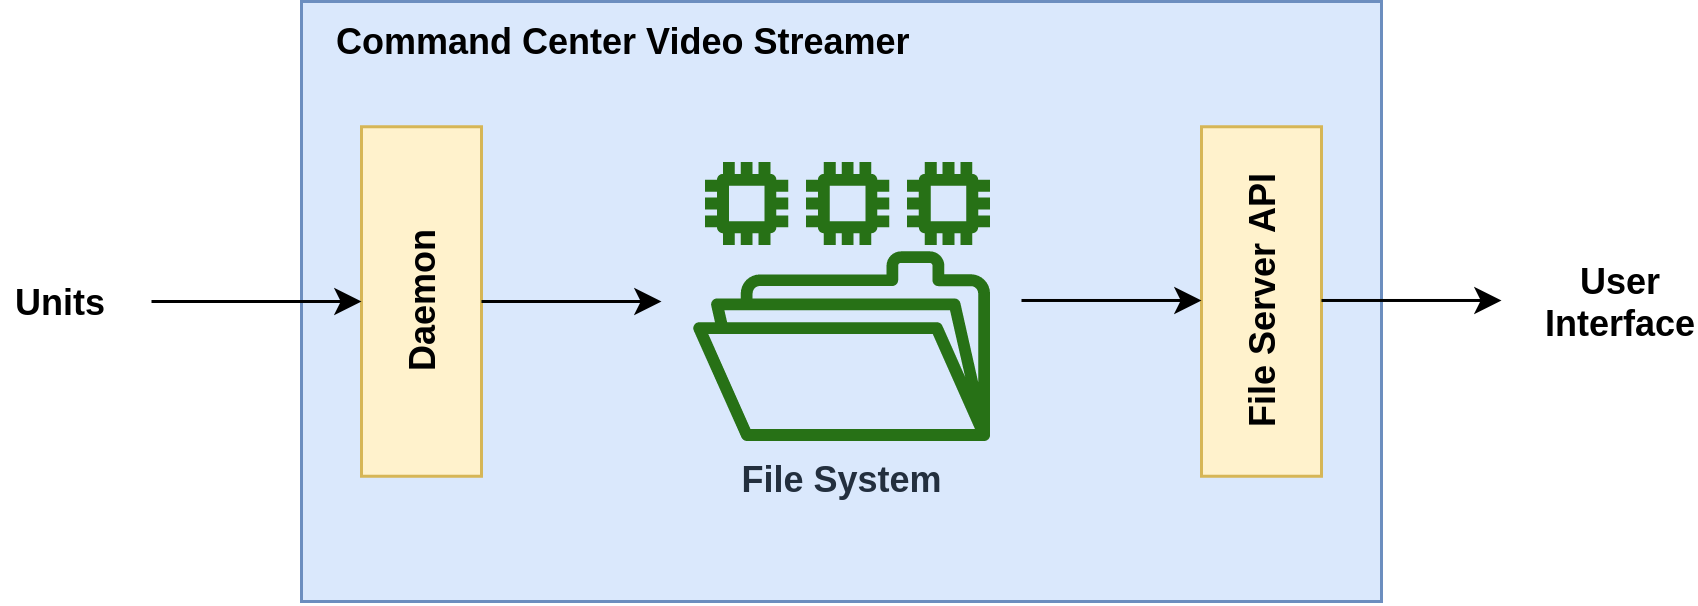
\includegraphics[width=\linewidth]{images/video-streamer.png}
    \caption{Video Streamer Data Flow}
    \label{fig:video-streamer}
\end{figure}

\subsubsection{User Interface}
The user interface in command center client allows operation leaders to manage and visualize units data, as well as record command audios and choose command codes that they want to send to these units.
There is two-way communication between the command center client daemon and the user interface. Data that recently arrived at the command center daemon is sent directly to the user interface using \acrfull{sse} to be visualized immediately to the operation leaders. While the data history is sent from command center daemon to user interface using \acrfull{rest} \acrshort{api} endpoints. 

Command center user interface is divided mainly into four pages: a login page, a map page, a units page, and finally a streams page. 
The login page is used to authenticate the operation leader to prevent masquerade attacks, as shown by Figure \ref{fig:cmd-ui-login}.

\begin{figure}[!htb]
    \centering
    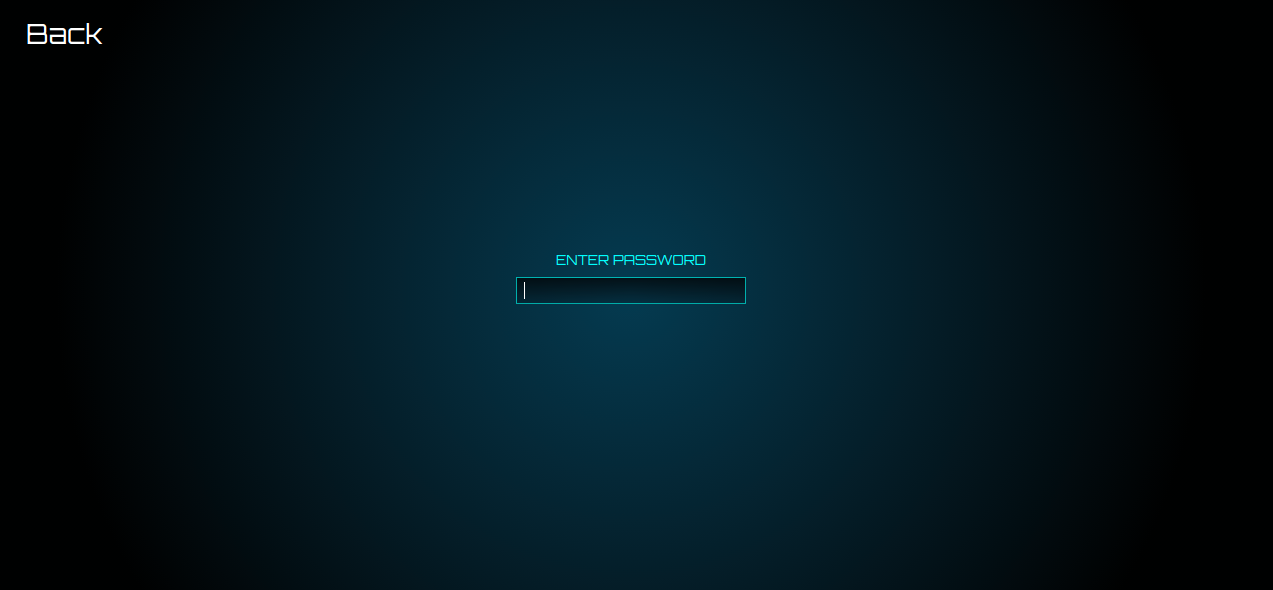
\includegraphics[width=15cm]{images/cmd-ui-login.png}
    \caption{\acrshort{cmd} \acrshort{ui} Login}
    \label{fig:cmd-ui-login}
\end{figure}


The map page is where the operation leader can view all nearby units' precise positions on a real map, as shown by Figure \ref{fig:cmd-ui-map-ch4}. Each unit is color-coded according to the group it belongs to, assisting the operation leader in analyzing group movements. When some unit sensor data indicates that this unit is in danger, or when some unit was inactive for more than two minutes and did not provide any sensor data during that time, the operation lead is informed. Any communications received from neighboring units are shown in a chat window. As soon as the data reaches the user interface, there will live update at the command center's screen. 

\begin{figure}[!htb]
    \centering
    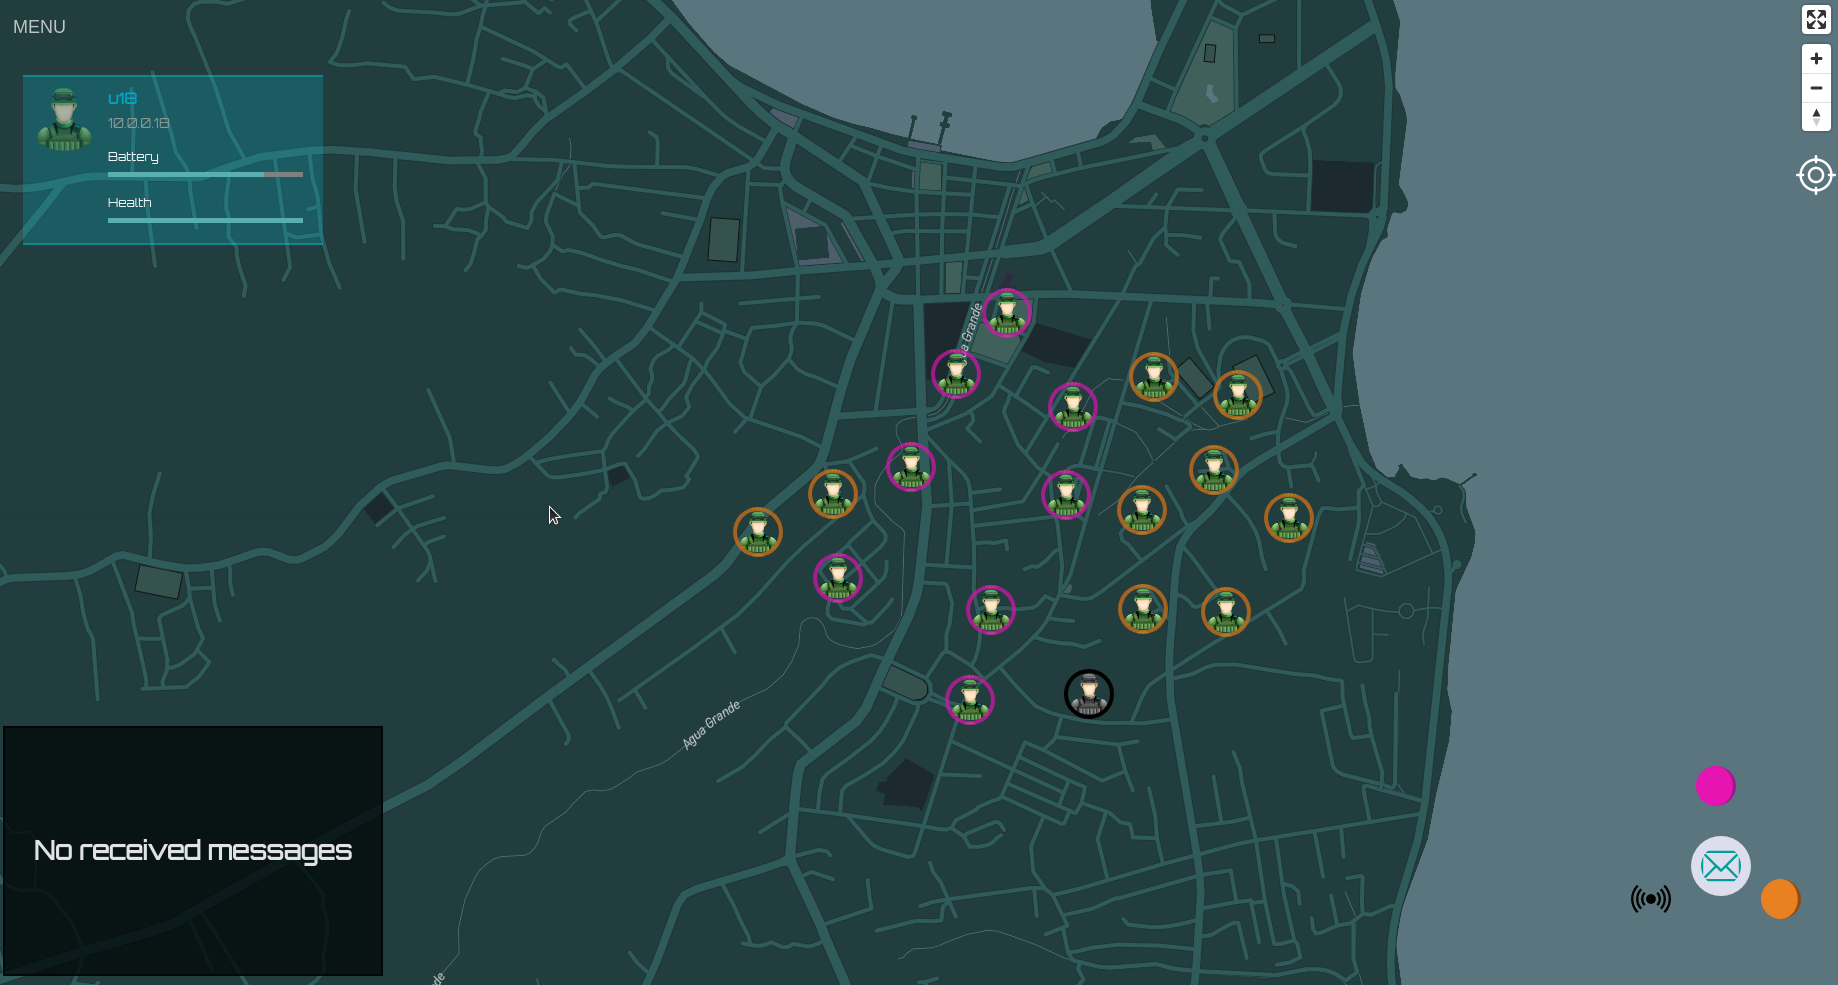
\includegraphics[width=15cm]{images/cmd-ui-map.png}
    \caption{\acrshort{cmd} \acrshort{ui} Map}
    \label{fig:cmd-ui-map-ch4}
\end{figure}


The operation leader can use the unit page (in Figure \ref{fig:cmd-ui-units-ch4}) to examine all of a unit's data history or send voice or message orders to it. All audios, videos, messages, position history, and sensors data of a unit are visible to the operation leader. 

\begin{figure}[!htb]
    \centering
    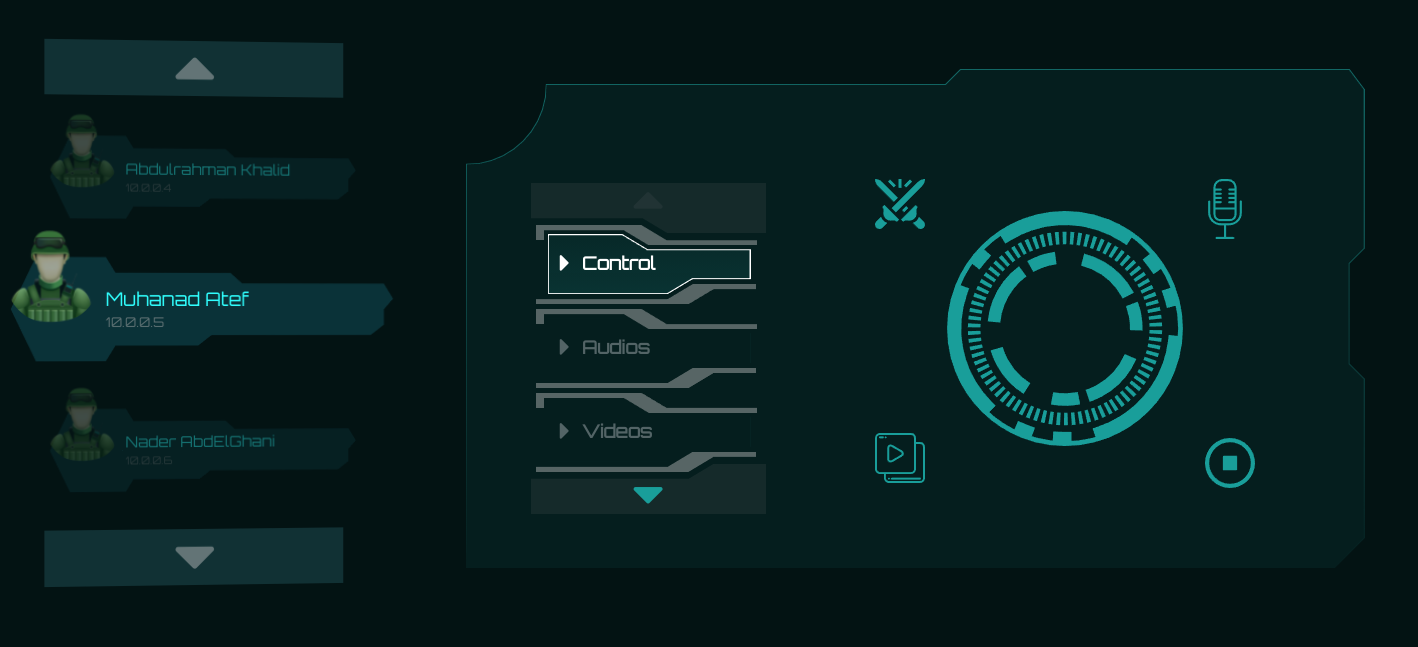
\includegraphics[width=15cm]{images/cmd-ui-units.png}
    \caption{\acrshort{cmd} \acrshort{ui} Units}
    \label{fig:cmd-ui-units-ch4}
\end{figure}


Finally, the operation leader may examine all live streams received from any nearby unit on the Streams page. This is shown by Figure \ref{fig:cmd-ui-streams-ch4}

\begin{figure}[!htb]
    \centering
    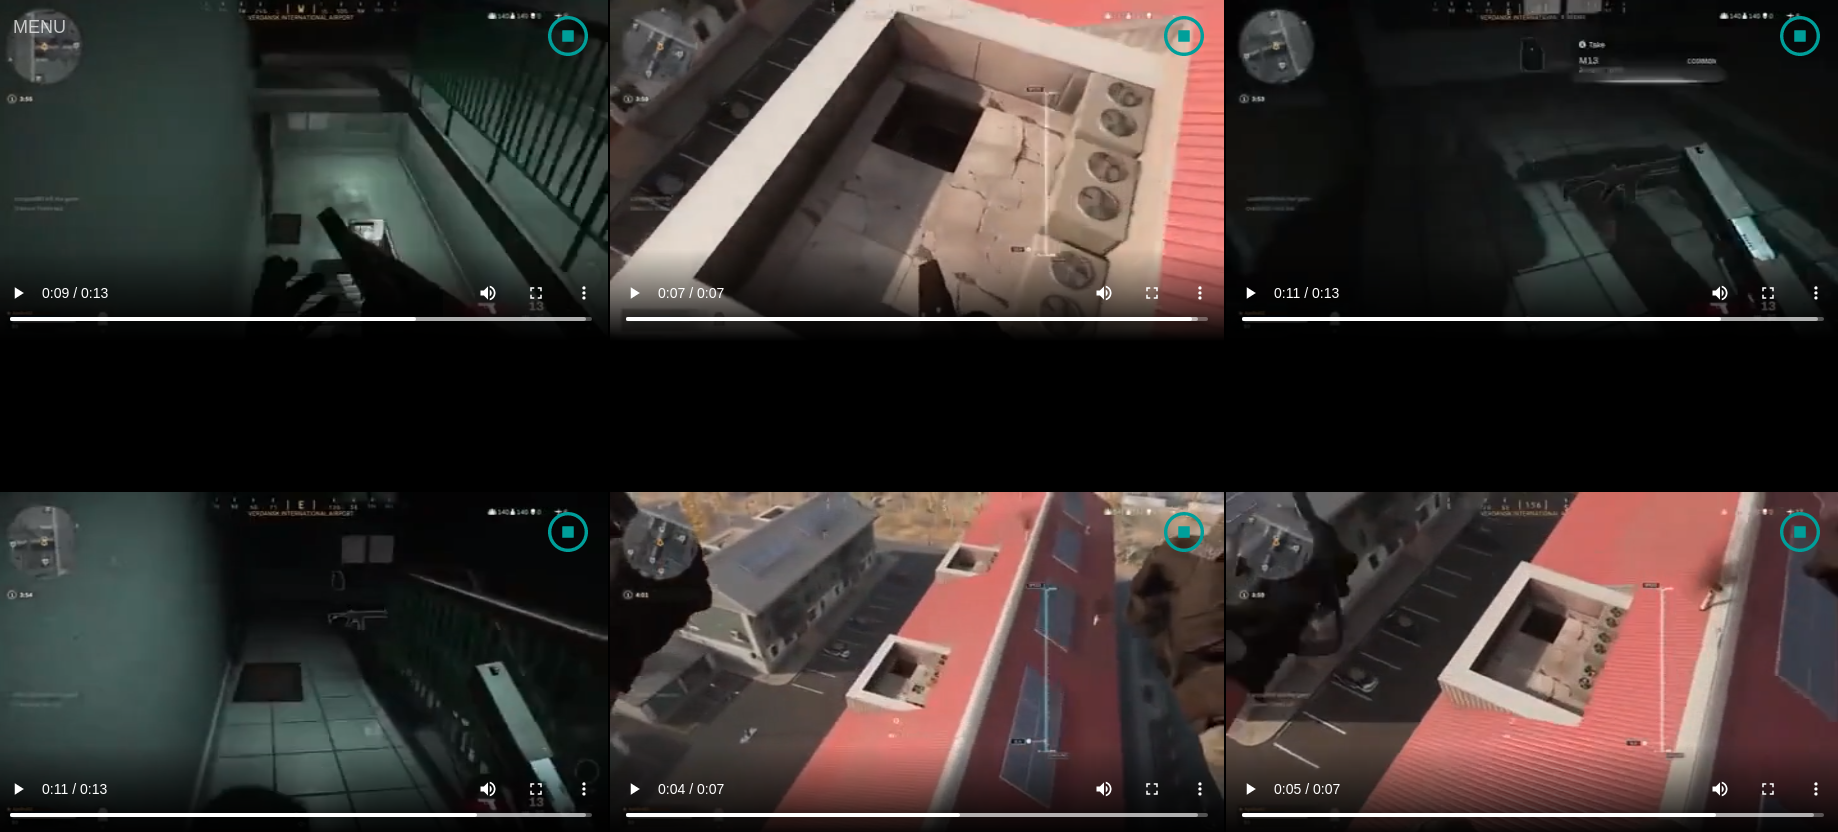
\includegraphics[width=15cm]{images/cmd-ui-streaming.png}
    \caption{\acrshort{cmd} \acrshort{ui} Streams}
    \label{fig:cmd-ui-streams-ch4}
\end{figure}


\section{Unit Client}
The unit client is the software that runs on the unit device, which is carried by the deployed soldiers and officers on the operation field.
More detail about the unit device in \ref{subsubsec:units-dev}.

\subsection{Functional Description}
\begin{itemize}[itemsep=1pt, topsep=5pt]
    \item Stream video from combat cameras to command center(s) only if the latter requested them. Video streaming terminates if the unit received an end-stream request, or the start request wasn’t refreshed after 1 minute.
    \item Stream the heartbeat and location of the device owner and their position every 10 seconds.
    \item Store all the recorded video and sensors (location and heartbeat) data locally.
    \item If the device user requested:
        \begin{itemize}[itemsep=1pt, topsep=5pt]
            \item Send audio messages from the microphone.
            \item Send code messages (every code has its predefined meaning.)
        \end{itemize}
    \item Receive audio messages from command centers into a queue.
    \item Play received audio messages from the queue instantly.
    \item Receive and show code messages.
\end{itemize}

\subsection{Modular Decomposition}
Figure \ref{fig:unit-modules} shows the modules of the unit client.

\begin{figure}[!htb]
    \centering
    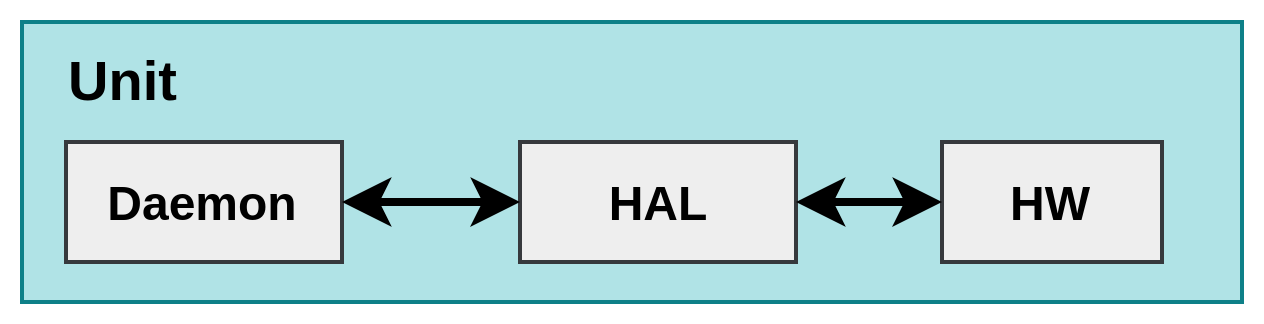
\includegraphics[width=11cm]{images/unit-modules.png}
    \caption{Unit Modules}
    \label{fig:unit-modules}
\end{figure}

The unit daemon implements the main state machine and logic of the unit.
It communicates with the daemon of the command center and transfers messages, whether they were audio or codes or streaming requests.

\acrfull{hal}, this abstracts the hardware, so we don't need to touch the unit client when porting to a different \acrshort{hw}.
It also serves the purpose of emulating the unit client \acrshort{hw} without the unit being aware of that.

\acrshort{hal} is responsible for streaming video from the camera source, or a video file in case we are testing.

\subsection{Design Constraints}
The unit runs on battery powered devices, so it needs minimal power and CPU consumption.

We lowered the CPU footprint by requiring \textit{FFmpeg} to generate only one level of quality for the video stream.
Also, we require that the command center should send stream request periodically to keep the stream. This is useful in case the command didn't want a stream, but the unit didn't receive its end video streaming request.

\chapter{System Testing and Verification}
\label{ch:system-testing}

This chapter introduces you to the testing setup and how we tested each module in isolation and the end-to-end integration that we planned and followed to prove to a high certainty the correctness of the system.

Testing ad-hoc networks always has been very tricky subjects, with researchers spending big amounts of funds on building testbeds with actual hardware and workers who move the hardware/devices around to change the connectivity between them.
It is a tedious task to test ad-hoc protocols on actual hardware.
The problem is harder when you want to execute the test multiple times.
It is very costly in terms of money and time and other resources.

This is why we took the decision, which some researchers take, and aimed to emulate the environment the system would likely be deployed on.
Most researchers take the path of network simulation, the difference is that with simulation, results are less accurate because of time compression and the lack of real world constrains like power consumption and latency while communicating with the kernel.
With emulation, we can run the protocol implementation in real time while integrating it with real kernel.
This enables us to explore how routing solutions could be built and constructed for real world systems, and let us face real world challenges regarding routing implementation.
Also, with emulation, we can run real applications on top of the router to test its performance.

Nevertheless, emulation lacks the capability of spawning big number of nodes due to the limits of computer's memory and because each node is an entire VM/container with real programs.
Kernel scheduler and memory management put limitations on the number of nodes' wireless devices we can emulate.

The next sections will walk you through our setup, scripts, GUIs and plans to prove the correctness of the programs we built in \acrshort{caian}.

\section{Testing Setup}
\subsection{Mininet-Wifi}
Mininet-Wifi is a python program and library that emulates wireless networks in infrastructure and ad-hoc modes.
It's a wrapper around Mininet project, which aims to emulate software defined networks for research and education.
It relies on \textit{wmediumd} and \textit{mac80211\_hwsim} kernel modules to simulate wireless radio devices and uses network namespaces feature from Linux to isolate processes as if they are in their own device.

With \textit{wmediumd}, Mininet-Wifi can simulate the propagation of wireless signals and control the probabilities of dropping packets and adding noise to them. 

Figure \ref{fig:mininet-diagram} shows unit and command nodes running inside a testbed created by Mininet, each node should have a router process.

\begin{figure}
    \centering
    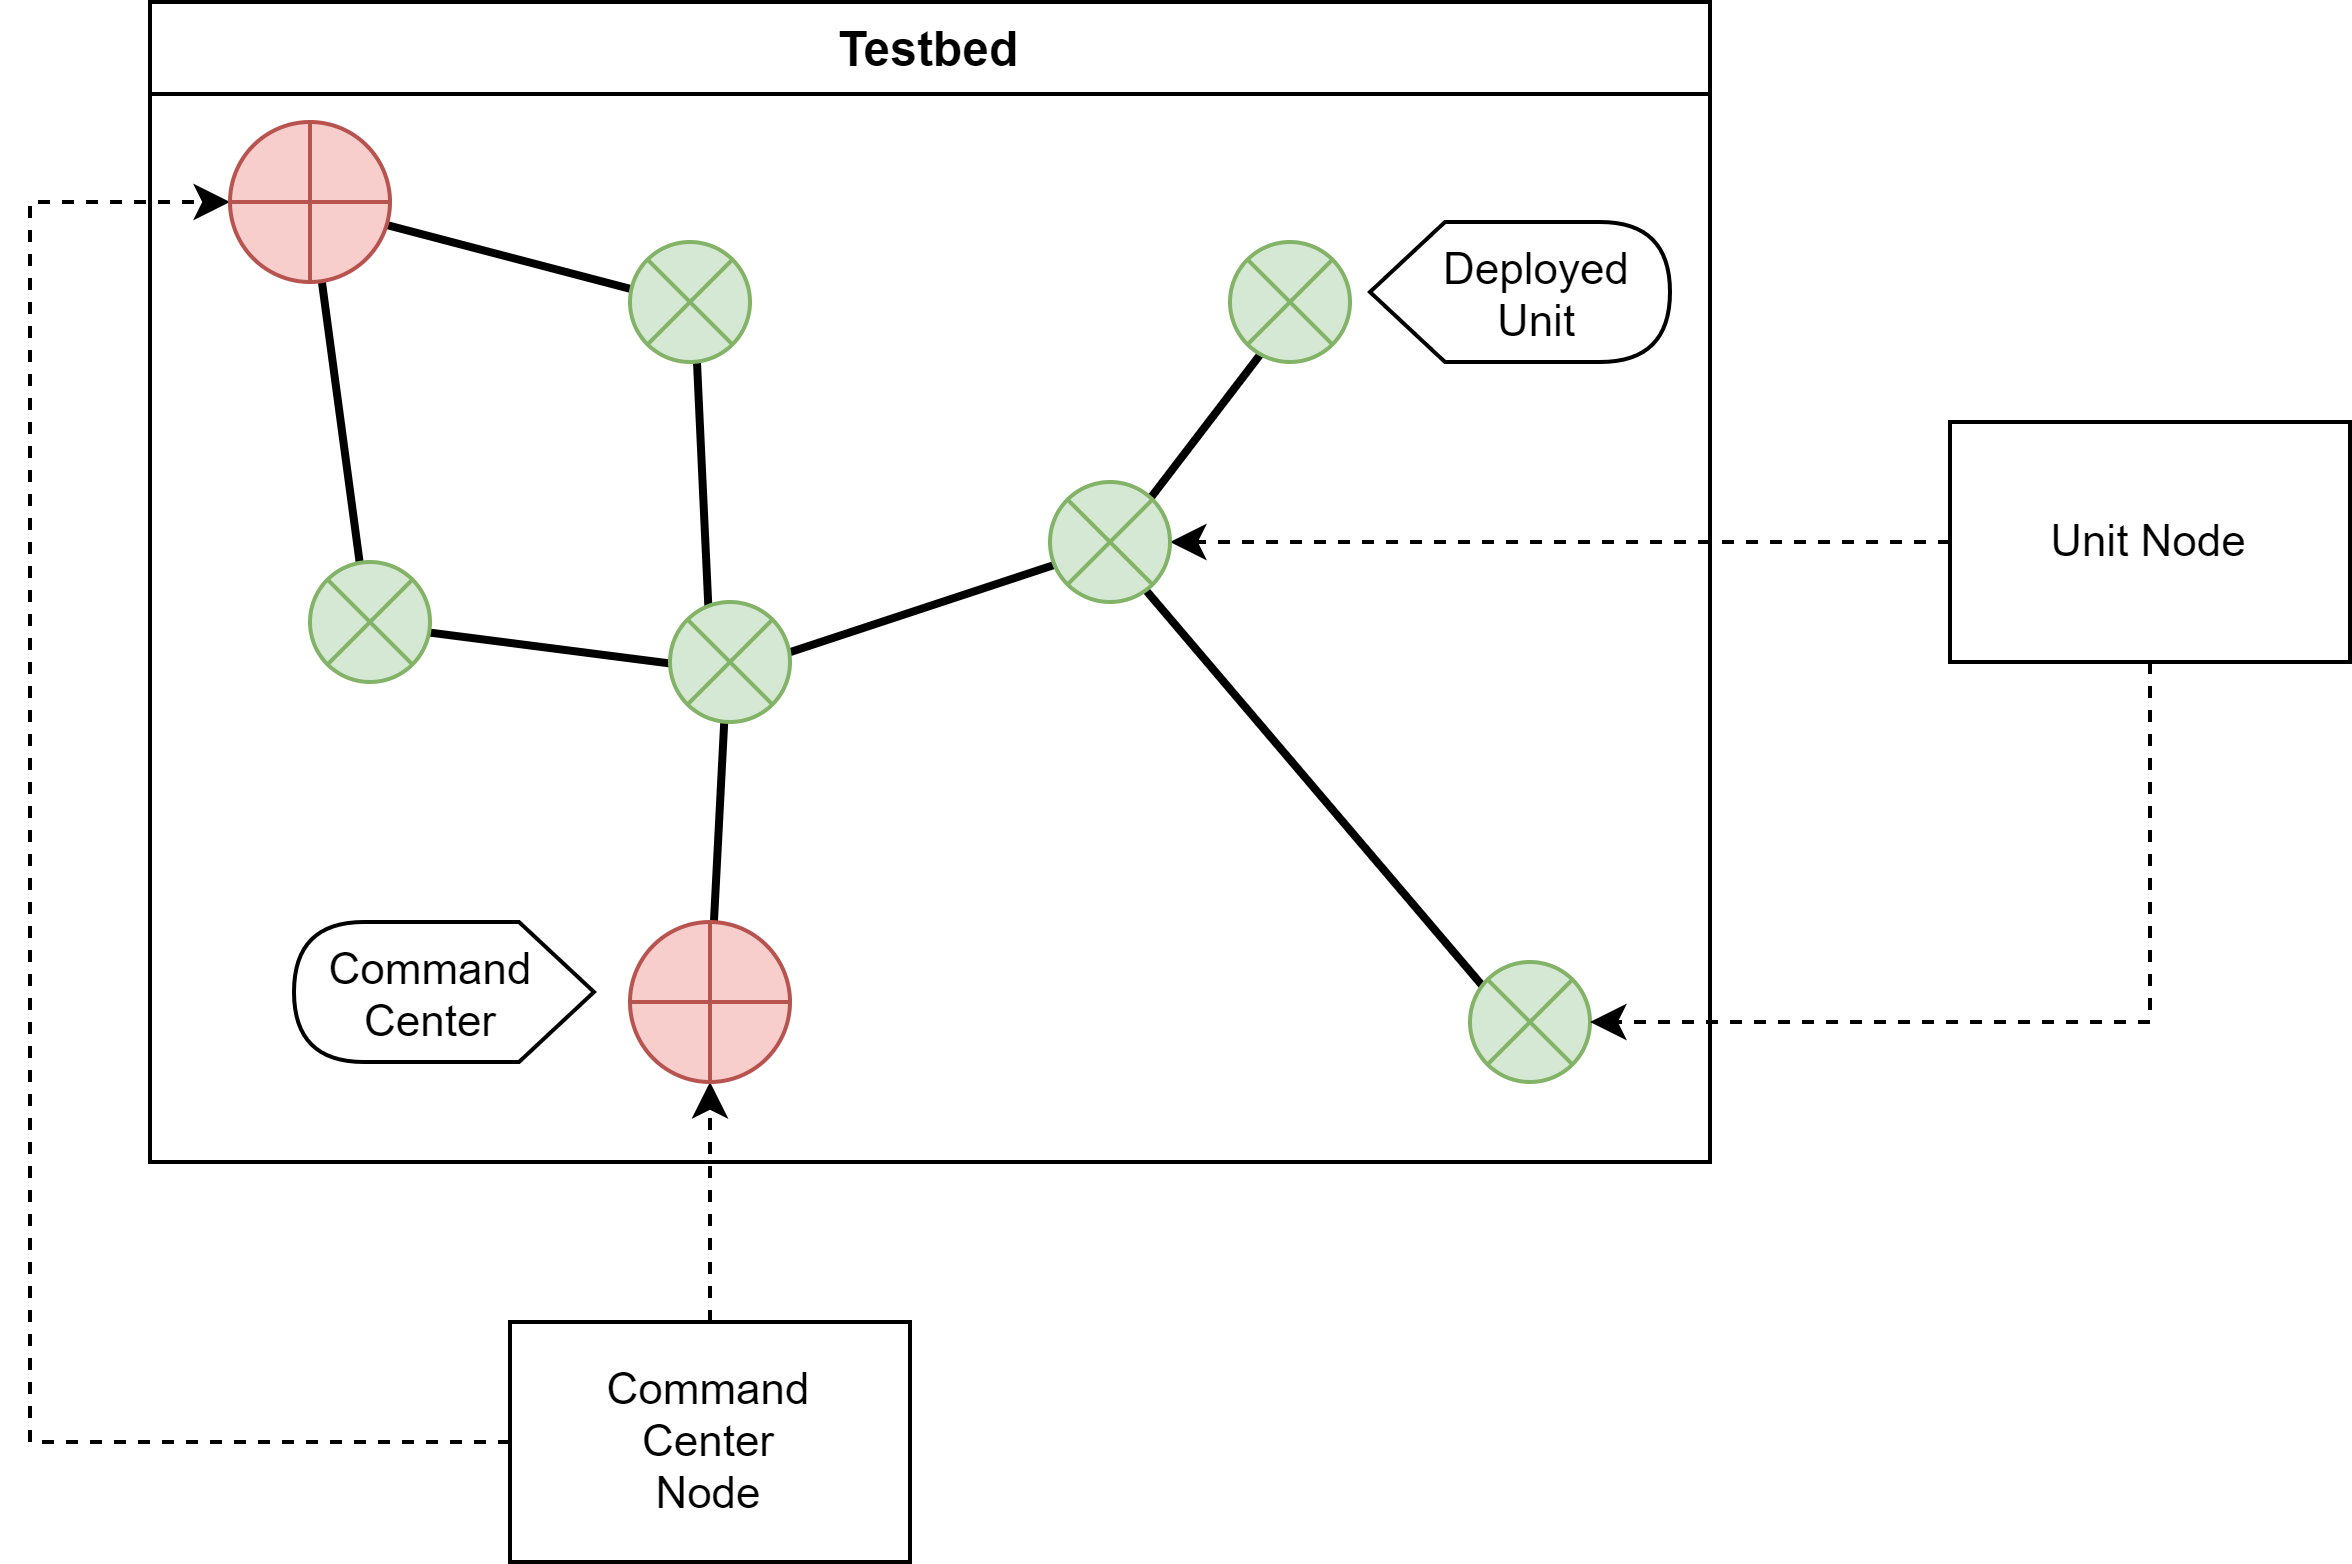
\includegraphics[width=13cm]{images/nodes_diagram.png}
    \caption{Mininet Testbed With Different Nodes}
    \label{fig:mininet-diagram}
\end{figure}

\subsubsection{Installing Mininet-Wifi}
Run the following:
\begin{verbatim}
$ python --version
\end{verbatim}

If it's 3, you are good to go, otherwise do the following:

\begin{verbatim}
$ sudo mv /bin/python /bin/python.old
$ sudo ln /bin/python3 /bin/python
\end{verbatim}

It may break your system, in this case reverse it back: 
\begin{verbatim}
sudo m /bin/python.old /bin/python
\end{verbatim}

Then install mininet-wifi:

\begin{verbatim}
$ (
    set -e
    sudo apt update
    sudo apt install -y git
    cd /tmp
    git clone git://github.com/intrig-unicamp/mininet-wifi
    sudo mininet-wifi/util/install.sh -Wln
)   
\end{verbatim}

\subsection{Edit GUI and MN Script}
To be able to create, edit and visualize the topology either offline or online (while Mininet-Wifi is running), we created \textit{edit} which is a web GUI for the testbed. 

Figure \ref{fig:edit-ui} shows edit UI, it has a map with units each has its name and range, you can move/add/delete nodes and change the hierarchical zones \textit{Zlen} and apply a mobility simulation with some configuration while connected to Mininet.

\begin{figure}[!hbf]
    \centering
    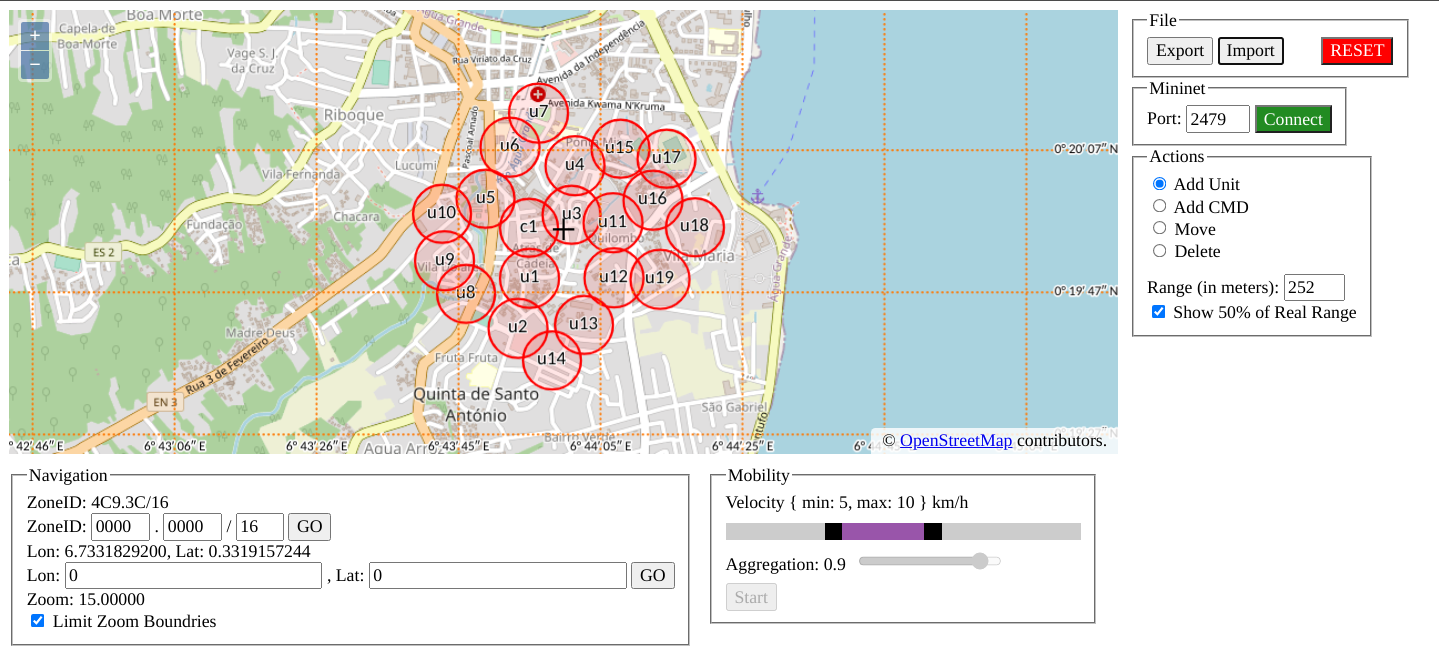
\includegraphics[width=15cm]{images/edit-ui.png}
    \caption{Edit GUI}
    \label{fig:edit-ui}
\end{figure}

Edit can export and import the topology into a specific format we made for the testbed.
Also edit can connect to a script we wrote that controls the routers and units and Mininet, edit gets updates about nodes' locations in case the script is moving them (while in mobility mode) or edit sends location updates in case the user is moving the nodes manually.

The script - called mn, written in python - uses a modified copy of pymobility which implements ``Time Variant Community'' Mobility or TVC for short, which works by defining a group of units and the model keeps them around some moving center it calculates.
This mobility model resembles the soldiers' units moving around, because most probably they won't walk randomly in different directions, but rather in groups together.

With ``aggregation'' control switch, you can in edit specify how much the group should move together, where 0 aggregation means every node is on its own.

The mn script sends the locations (longitude and latitude) for each node periodically through Unix sockets open by routers and units on the nodes.

\subsection{Start Script}
Start is a script that can any component of the system, whether it's on the localhost or inside the Mininet namespaces.
The following is how to run Mininet on some topology and routers and units and command centers' daemons and \acrshort{hal}s using start:
\begin{verbatim}
## (1st terminal)
# start mininet-wifi within chromosome topology
$ sudo ./start mn topos/chromosome.topo

## (2nd terminal)
# start routers in all nodes
$ sudo ./start routers

## (3rd terminal)
$ sudo ./start units
## (4th terminal)
$ sudo ./start cmds
## (5th terminal)
$ sudo ./start hals
\end{verbatim}

Start lists Mininet namespaces using pgrep, then injects programs into the Mininet containers using nsenter and watches for file changes using watchdog script.

\subsubsection{Socat}

The CMD UI and Unit UI can only communicate with their daemons using TCP sockets, but the daemons are isolated in the namespaces and running any GUI inside is tedious and maybe impossible (due to X11/Wayland using TCP sockets and residing outside the namespace) this is why we used \textit{socat} utility to forward TCP sockets in the host machine to Unix sockets that are exposed by the daemons.
Because Unix sockets are [virtual] files, and the namespaces are just network namespaces, the Unix sockets are not isolated inside the namespaces, so we could forward them into TCP sockets for the UI.
This helped us avoid changing the interface for the UI just to test inside the testbed.

Figure \ref{fig:socat-diagram} shows how the socket forwarding happens with the testbed.

\begin{figure}[!hbf]
    \centering
    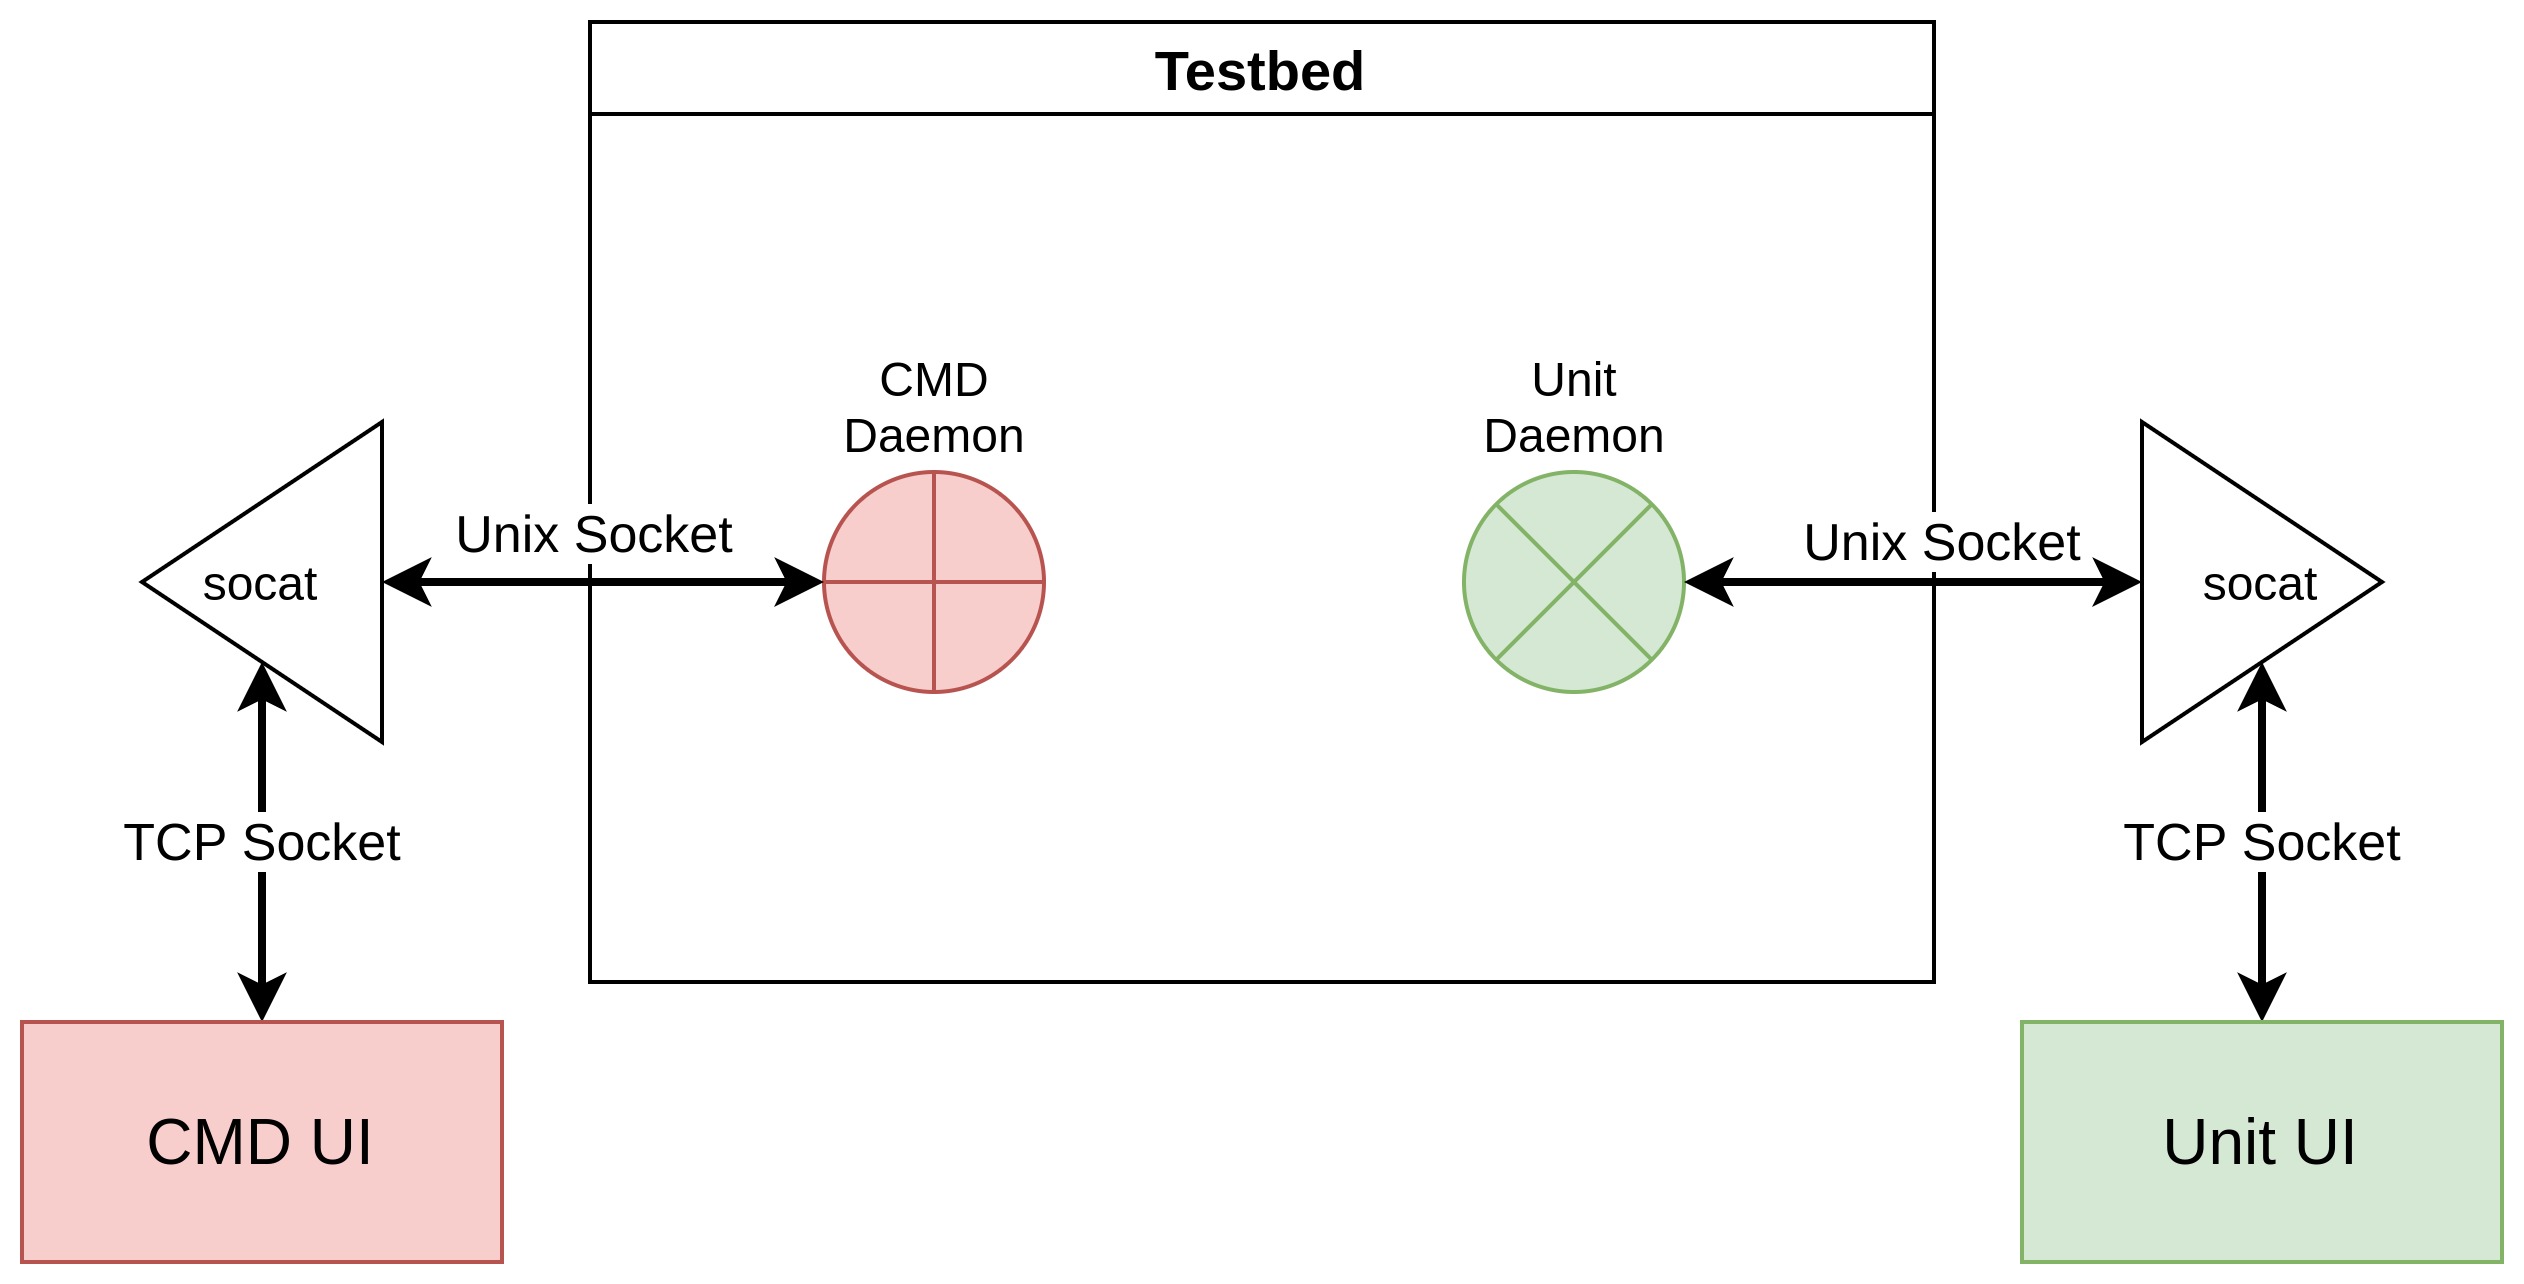
\includegraphics[width=13cm]{images/socat-diagram.png}
    \caption{Socat Forwarding and UI}
    \label{fig:socat-diagram}
\end{figure}

\section{Testing Plan and Strategy}
Our main goal in evaluating each module in \acrshort{caian} was to make sure it met all functional and non-functional requirements that were specified earlier. Testing is almost as challenging as development, if not more difficult in the world of networks, especially ad-hoc networks. We were very cautious from the very beginning of this project to provide a testing environment that allowed us to test each and every stage of the development process. For example, the sARP protocol was one of the first implemented protocols related to the Zone-based Hierarchical Link State (\acrshort{zhls}) unicast protocol; at this stage, we must ensure that the protocol is functioning properly, that each node can identify its neighbors, and that the delay metric to each of them is correctly measured.

For the reasons stated above, testing development could not be postponed after code development. As a result, our testing strategy was obvious from the start in terms of the need for a testing environment that allows us to construct multiple topologies with varied patterns of movement and exchange and route messages between different nodes in these topologies. \acrshort{caian} testing development plan can be mainly divided into three components as shown in Figure \ref{fig:testing-strategy}: \acrshort{utils} testing development, integration testing development and network testing development that serves both module and integration testing.

\begin{figure}[!hbf]
    \centering
    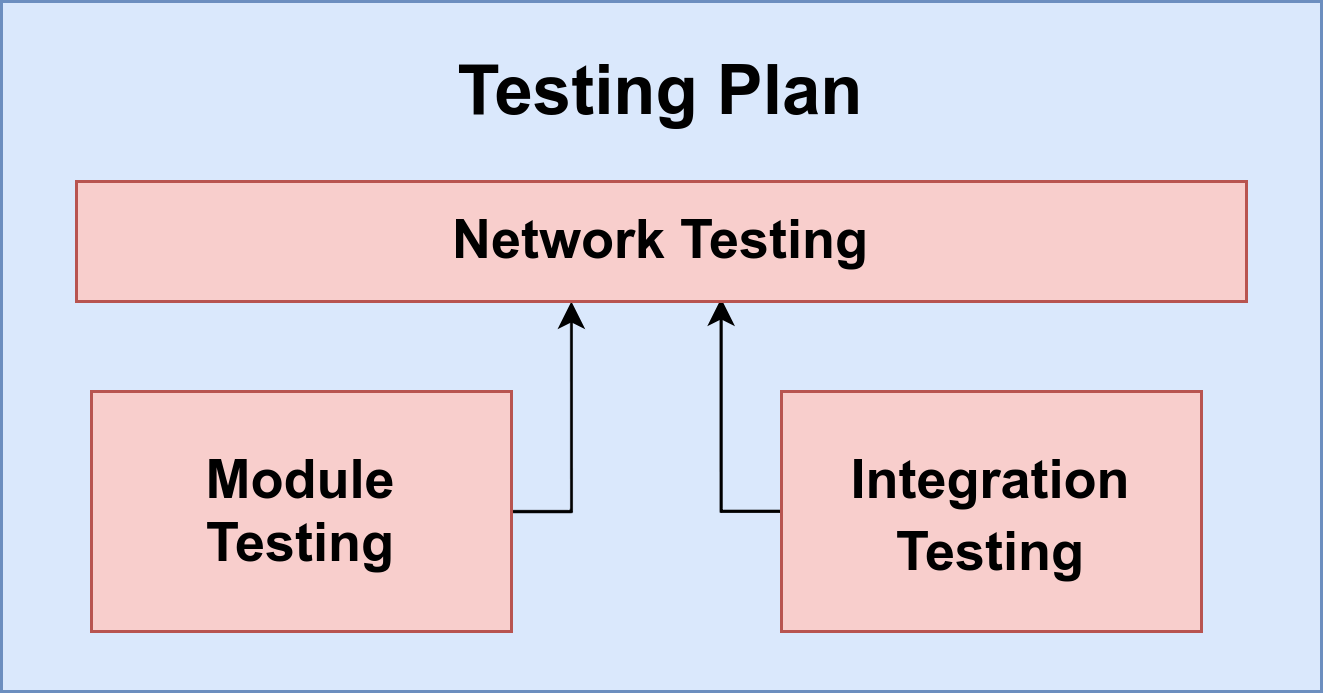
\includegraphics[width=15cm]{images/testing-plan.png}
    \caption{Testing Strategy}
    \label{fig:testing-strategy}
\end{figure}

Each component will be briefly discussed in the section below.

\subsection{Module Testing}
In \acrshort{caian}, Module testing is done sequentially into two steps as show in Figure \ref{fig:module-testing}: \acrshort{utils} testing and network testing. All protocols that need an active topology with several nodes, as well as the ability to relocate these nodes and encapsulate each in its own network namespace, fall under the network testing umbrella, and this type of testing development starts from the very beginning of our project. However, \acrshort{utils} testing was concerned with aspects that could be verified independently of the network, such as encoding, decoding, marshalling, unmarshalling, graph algorithms, tables handling, and timers. This type of testing was developed immediately after the development of its related code.

\begin{figure}
    \centering
    \includegraphics[width=15cm]{images/module-testing.png}
    \caption{Module Testing}
    \label{fig:module-testing}
\end{figure}


\subsection{Integration Testing}
Integration testing was a difficult process in \acrshort{caian}. It contains end-to-end testing using a topology that has numerous of nodes, each with its own user interface and router.

The integration testing was split into two primary procedures that ran simultaneously. The initial step was to evaluate the app's functionality from units to command centers and back. This process was carried out both automatically using \acrshort{hal} scripts to simulate units and send periodic sensor data and stream videos to the command center, as well as manually to test both unit and command center user interfaces and ensure that multicast and broadcast data was sent only to its intended destination.

The second step in the integration testing process was to test the routing decisions. Data delivery to its intended destination wasn't enough for us to declare that the system functioned as it's intended to be. It was critical to observe and evaluate each node's routing choice, as well as how data is delivered from its source to its intended destination. To accomplish so, we created a log visualizer software as shown in Figure \ref{fig:log-vis} that can collect all the router logs and evaluate their forwarding decisions, and displaying them to us in a way that allows us to appraise the router's performance and behavior. 

\begin{figure}[!hbf]
    \centering
    \includegraphics[width=7cm]{images/log-vis1.png}
    \includegraphics[trim={0 0 0 1.3cm},clip,width=7cm]{images/log-vis2.png}
    \caption{Log Visualizer}
    \label{fig:log-vis}
\end{figure}


\section{Comparative Results to Previous Work}
Table \ref{tab:comparison-table} shows the difference between our work and previous work.
We introduced new concepts and extensions to the protocols and implemented them.
All the extensions have been discussed in great detail throughout the book.

\begin{table}[!htb]
\centering
\resizebox{\textwidth}{!}{%
\begin{tabular}{|c|c|c|c|}
\hline
Protocol              & Comparison            & Previous Work           & Our Work       \\ \hline
 & Zone Size             & Constant and Predefined & Variable       \\ \cline{2-4} 
       \multirow{-2}{*}{ZHLS}               & Maintained Topologies & Two Separate            & Single Unified \\ \hline
Broadcast             & Limits                & Unbounded               & \begin{tabular}[c]{@{}c@{}}Geographically Limited \\ with a Radius\end{tabular} \\ \hline
ODMRP                 & Join Query            & Using Flooding          & \begin{tabular}[c]{@{}c@{}}Iterating Over \\ Next Hops\end{tabular}             \\ \hline
\end{tabular}%
}
\caption{Summary of Differences Between Our Work and Previous Work}
\label{tab:comparison-table}
\end{table}


\chapter{Conclusions and Future Work}

% This chapter should summarize the whole project, it features and limitation. Moreover, you should give directions for future work

% In this space, before the first section, write an introductory paragraph for the chapter

We have introduced \acrshort{caian} as a communications solution for tactical teams, and thoroughly explained how it works. In this chapter, we let you catch a glimpse of how our journey looked like. We describe the challenges that we faced, the lessons that we learned, and summarize what we achieved. Finally, we discuss what the future may look like for \acrshort{caian}.    

\section{Faced Challenges}
% Mention all the problems/challenges that you faced while working with the project and how you overcome them

The core of \acrshort{caian} is the router. Routing in \acrshort{manets} is a research problem that has no established solutions. A multitude of routing protocols are being researched, with only a few implementations. Working on such a problem has introduced us to a variety of challenges.

\subsection{\acrshort{manet} routing}
Routing in \acrshort{manets} is an open-ended research problem that we had no background of. We needed to accumulate the necessary background knowledge through research papers and books. Afterward, we had to choose and tune adequate routing protocols for our project. We began our journey through literature, understanding and comparing different approaches until we were able to select candidate protocols. Moreover, The papers explaining routing protocols focused on theory. As no open-source implementations exist, we had to fill in the missing pieces during our implementation.

\subsection{Interfacing with Linux Kernel}
The router module works in layer 3 of the TCP/\acrshort{ip} network stack. Ideally, it would be implemented as a kernel module that replaces \acrshort{ip} routing in Linux. This approach comes with a huge implementation overhead of learning kernel modules, debugging the kernel, and others too many to list. To stay focused on the routing problem, we decided to run the router in user mode. In order to be able to implement routing in user mode, we needed to intercept and re-inject packets at different layers of the Linux network stack. This involved understanding different interfaces offered by the Linux network stack, and a few hacks and tricks to be able to achieve the necessary task in user mode.

\subsection{Testbed}
We decided not to use a simulation for our project, to implement a fully-functional product. However, we still needed a testbed that runs multiple nodes with different topologies and mobility models. Creating the testbed involved writing complex scripts to run multiple instances of the project in separate network namespaces and be able to communicate with them from the default namespace to run the user interfaces, and using a tool called Mininet-WiFi that provides emulated wireless interfaces to simulate connectivity between nodes. Mininet-WiFi was one of a very few available options, so we had to adapt our needs to the tool and its shortcomings.

\subsection{Testing and Debugging}
Testing and debugging the project is not easy, as we are debugging a whole network at once. Even with a small-sized network, troubleshooting involves running several instances at once and tracing their logs concurrently (especially when debugging multicasting). Furthermore, we had to develop a simple \acrshort{gui} that renders the nodes as they move through different zones on a map, to help us create and debug different topologies.

\subsection{Performance Metrics}
\acrshort{caian} is implemented as a fully functional program in user space. Other implementations of research papers are only implemented in simulation, while the few publicly available fully functional implementations run in kernel space, and without encryption. This fact made acquiring any performance metrics and testing against other routing solutions almost impossible. The lack of open source implementations of \acrshort{manet} routing solutions combined with the lack of proper tools to emulate large enough mobile ad-hoc networks for testing is disappointing. 

\section{Gained Experience}
% Mentioned the experience/skills that you gained from working with the project

Working on developing \acrshort{caian} has been an enriching experience that we learned from in different ways:
\begin{itemize}[itemsep=1pt, topsep=5pt]
    \item We gained a deeper understanding of networks and routing, especially \acrshort{manets}.
    \item Exposure to research papers and being up-to-date with the advancements in \acrshort{manet} routing.
    \item Reasoning about protocols and choosing the practical ones, keeping trade-offs in mind.
    \item Navigating and understanding protocols \acrshort{rfc}s.
    \item Writing highly concurrent programs.
    \item More experience with low-level implementations and interfacing with Linux.
    \item We learned several tools and technologies such as \textit{Golang} and \textit{Electron.js}. 
    \item Teamwork, effective collaboration, and asynchronous online communications.
\end{itemize}
\section{Conclusions}
% Write your conclusions regarding the project. Mention its features and limitations

Routing in \acrshort{manets} is a research problem that is yet to have solid implementations. \acrshort{caian} as a system implements unicast routing, multicast routing, and broadcast routing. It is one of a very few concrete open source implementations. It offers reliable communications without infrastructure. Nonetheless, it does have its limitations. Due to the lack of proper tools, \acrshort{caian} is yet to be tested on a very large scale. Introducing scale introduces problems, and stress testing \acrshort{caian} in a very large network is something that we do not have the proper tools to do at the moment. Moreover, \acrshort{caian}'s current implementation only runs on Linux, It is not a cross-platform solution. 

\section{Future Work}
% Give possible extensions, enhancements and future work of you project, such that subsequent students could build on your work and develop larger systems/platforms.

\acrshort{caian} is one of a few of its kind. It can be extended and built upon in many ways in the future. In this section, we list a few ways in which \acrshort{caian} can be extended.

\subsection{Hardware Deployment}
Currently, \acrshort{caian} is a software system that provides communications to tactical teams. The system can be deployed on any Linux-based platform for more realistic testing and benchmarking. Moreover, the router can be used for any other application involving \acrshort{manets}. The system can be extended with proper software clients to be used for communication in fleets of autonomous vehicles or robots.

\subsection{Multicast Support for TCP}
One possible large-scale extension is to build a multicast variation of TCP. Since the scope of our project was concerned with routing, we did not have time to work on such a transport layer protocol. Multicast support for TCP is also a research problem, with no deployed protocols on Linux. The lack of support for TCP in multicasting has restricted our ability to make the most out of multicast routing. If implemented, the use cases of \acrshort{caian} can be extended to support reliable delivery of messages and audio to multiple units at once.

\subsection{Alternatives to Mininet-WiFi}
Mininet-WiFi is a great tool that enabled us to test our system with a variety of topologies. 
Nonetheless, it has its shortcomings. 
Mininet-WiFi limits the number of nodes that we can use to 100 nodes, which can be a problem when testing for scalability. 
Furthermore, the way Mininet-WiFi handles mobility and node ranges is a little cumbersome. 
At the time of writing, we did not find any better alternatives. 
If a better alternative comes up in the future, it may be worth switching the testbed to use it.

We might need to write our own alternative.
At the end, Mininet-Wifi is a wrapper around \textit{wmediumd} and \textit{mac80211\_hwsim} which are simple enough to be improved for better networks emulation and for support for more virtual radios.

\subsection{Uniform Shapes for Hierarchical Zones}
In \acrshort{caian}, zones are hierarchical and have a rectangular shape. Using more uniform shapes such triangles and hexagons will make zones at the same level have more consistent areas. However, the zone computations will be less straightforward and may be more CPU intensive, which could hurt the limited battery capacity in the handheld devices.

We need to explore the tradeoffs in this area.

\subsection{Implementing The Router as a Kernel Module}
A kernel module is a piece of software that runs in the kernel, it can call any kernel functions and access its data directly with the highest privileges in the system.
The advantage of writing a kernel module for the router is that kernel modules don't cause overheads while accessing packets and modifying them.
Because they are in the kernel side, they can access the packet buffer directly and modify it in place, which means it takes less time than doing the same in the user space, as the later needs copying from kernel space to user space and back again after the router finishes the packet task.

On the other hand kernel modules are not safe, because if they caused a failure, you won't simply restart it, you might have to restart the whole machine, and maybe even enter a broken state of the whole system where nothing functions and it requires a manual intervention, which is not ideal for a software that might be updated very rarely and be required to function for the most number of continues hours and be very reliable.

Also, if the kernel module has a small bug, it might be a big security hole and might give the attacker a control over the whole system silently.
On the other hand, the same bug on the user space might be abused for a small limit.
Thus, writing programs for the user space is much safer and secure.

This is a trade-off between performance and security.
And we chose security and safety.

Nevertheless, the performance hit, due to copying back and forth, might be small.
But we need to assure that by writing a small part of the router in the kernel space and compare the differences.
At the end, we might not need to write the whole router in the kernel.
We may just write the part that encrypts the packet and adds \textit{\acrshort{zid}} and let it copy the packet's header to user space to decide its forwarding destination, this might reduce the performance penalty.

Doing reactive routing with Linux's forwarding tables is tricky, we also need to explore how to deal with this without user space router.

\subsection{Forwarding with \acrshort{ebpf}}
Writing a kernel module is risky because it may damage the whole system for one small bug.
Kernel modules are not isolated, and if compromised, the whole system is compromised.
Thus \textit{\acrshort{ebpf}} is introduced.

\acrfull{ebpf}, which found on most \textit{UNIX} operating systems and developed lately for Microsoft Windows.
It's an interface for user space programs to insert code that runs safely in the kernel.
This code can filter syscalls, packets and events on the kernel and operate on those data.
The safe part of \acrshort{ebpf} is that all code is executed in a virtual machine, and before executing them they are verified to not access any unauthorized data or cause any memory leaks or destroy any memory it doesn't hold.

\acrshort{ebpf} may speed up forwarding as it can just operate on the kernel space directly and thus safe time of copying packets back and forth.
Also, they are generally much safer than writing kernel modules directly, thanks to the verification system and the virtual machine.

BPF was designed first for networking applications, and later came the extensions which serve other applications, like security and syscalls modifications, that seek high performance integration with the kernel functionality.

We might need to explore using \acrshort{ebpf} for the forwarding plan on the performance of the router.

\subsection{No FFmpeg}
Currently, we use \textit{FFmpeg} for video streaming.
We give it the video source, let it be a camera stream or a video file or a URL for another stream, and it cuts it into \acrshort{hls} chunks and produces \texttt{.m3u8} metadata files which we move around to the frontend player.

We may reach a better user experience by reducing the complexity of the code base, and instead of calling another program, which has its downsides of how to deal with evens back and forth between the producer and consumer of the \acrfull{hls} segments which we fixed in a non-ideal way.
We might implement our own \acrshort{hls} segmenter, which just segment the video source in memory directly and serve with minimal latency.

\subsection{Different Quality Levels of Streaming}
Currently, the unit daemon only streams at one level of quality, this is for simplicity.
But we might need to have multiple available streams with different qualities for each one.
\acrshort{hls} already supports this, but the problem resides in the power and memory tradeoffs against the performance, given that the unit devices have limited capacity for battery.

We might need to try a different approach than the one \acrshort{hls} took.
If the network and battery are in good conditions, the CMD daemon gets notified of the availability of streaming at a higher quality, and they may select a higher quality if they wanted to which the unit reacts to by encoding and streaming at the selected quality level.

This is different from what \acrshort{hls} does, which is making all the levels available proactively.
Clearly, \acrshort{hls}' approach is not suitable for handheld devices, and we need a reactive approach.
This may require us to extend the protocol.

\newpage

\printbibliography

\begin{appendices}
\chapter{Development Platforms and Tools}
\section{Hardware Tools }
Personal computers running linux-based oberating systems.

\section{Software Tools}
\subsection{Programming Languages}
\subsubsection{Golang}
Go was created at Google to help programmers be more productive in an era of multicore, networked devices by including the following features: 
\begin{enumerate}[itemsep=1pt, topsep=5pt]
    \item Run-time efficiency (like C).
    \item Multiprocessing and high-performance networking.
    \item Readability and usability are two of the most important factors to consider (like Python).
\end{enumerate}
\textbf{Usage:} Main programming to build the core modules and daemons.

\subsubsection{Python}
Python is a high-level programming language that is interpreted and object-oriented. It's ideal for Rapid Application Development, as well as using as a scripting or glue language to link together existing components.
\\
\textbf{Usage:} To write testbed scripts

\subsubsection{Shell Scripting}
Shell scripting is a type of scripting that runs in the Unix/Linux shell.
It can condense long and repeated command sequences into a single, easy-to-understand script.
\\
\textbf{Usage:} For running repetitive commands with a single script.

\subsection{Libraries and Frameworks}
\subsubsection{Mininet}
Mininet builds a realistic virtual network on a single system, running actual kernel, switch, and application code.
\\
\textbf{Usage:} For testing our system with a variety of topologies.
\subsubsection{Socat}
Socat is a command-line utility for creating and transferring data across two bidirectional byte streams.
\\
\textbf{Usage:} For forwarding data from TCP to Unix sockets to make the user interface works on the browser, however the daemons are running inside containers without changing the interfacing.
\subsubsection{Nsenter}
It's a simple utility that lets you enter namespaces.
It can technically enter existing namespaces or start a new process in a different set of namespaces. 
\\
\textbf{Usage:} For Running the programs inside containers.
\subsubsection{React.js}
React is a JavaScript library for creating user interfaces that is fast and adaptable.
\\
\textbf{Usage:} Build both Command Center and Unit user interface (UI) as a web application.
\subsubsection{Electron.js}
Electron.js is a runtime framework for developing desktop applications.
\\
\textbf{Usage:} Build both Command Center and Unit user interface (UI) as a desktop application.
\subsection{Tools and Platforms}
\begin{itemize}
    \item Visual Studio Code: it is a free source-code editor with debugging support.
    \item GitHub: it is an online service that hosts Git repositories for software development and version control. 
\end{itemize}

\chapter{Use Cases}
%Include all your use cases

C4IAN is designed to provide infrastructure-less wireless communications for tactical teams. It provides the following services for command centers and units, who can be moving freely:
\begin{itemize}[noitemsep, topsep=0pt]
    \item Exchanging code messages between units and command centers.
    \item Exchanging audio messages between units and command centers.
    \item Assigning units to groups, and sending audio messages from command centers to a specific groups (multicasting), or to all units (broadcasting).
    \item Streaming sensors' data (location, heartbeat, etc.) from units to command centers.
    \item Streaming videos from combat cameras at the units to command centers on-demand.
    \item Recording and visualizing all communications history with different units at command centers.
\end{itemize} 

\vspace{\baselineskip}

These services are provided by the implemented clients for command centers and units. However, the underlying router is a generic MANET router that can be easily used for further applications by modifying or extending the software clients. Some examples are:
\begin{itemize}[noitemsep, topsep=0pt]
    \item Controlling fleets of drones or autonomous vehicles.
    \item Providing communications for smart robots with decentralized coordination.
    \item Aggregating sensors data from moving vehicles.
\end{itemize}

\chapter{User Guide}
Prepare a user guide for your project. Ensure that the guide is clear, detailed and easy for an ordinary customer to use your project. Employ figures and charts as needed to facilitate the use of your guide

\chapter{Feasibility Study}

\quad  In this appendix, we discuss the feasibility of C4IAN. As chapter 2 covered marketing and financial aspects, we will focus on technical, operational, and legal feasibility.

\section{Technical Feasibility}

\quad To design C4IAN, a strong background in networks is required, especially mobile ad-hoc networks. The resources for learning networks are abundant, but those for mobile ad-hoc networks are scarce. Learning about routing in mobile ad-hoc networks and choosing adequate protocols to implement is not an easy task.

After the produce is designed, the implementation phase requires skills in low level programming. As the router module interfaces extensively with the Linux kernel, and it's network stack, knowledge about low level programming and networks programming is a must. Since the Linux kernel is open source, the implementation could be completed without major obstacles. The router could be implemented in user mode, or as a kernel module. Both are available options due to the flexibility of the Linux kernel. As Linux is a relatively lightweight operating system that can be deployed on various hardware, deploying C4IAN on most types of hardware should not be problematic.

\section{Operational Feasibility}

\quad From the user's point of view, C4IAN is a very easy system to operate. Most of the complexity is hidden in the router implementation, which the users (and the applications) do not directly interact with. The router module interacts exclusively with the Linux kernel. From the perspective of a user, or an application developer, the system is transparent. The implementation of applications is not affected by the design or implementation of the router. This gives a lot of flexibility for developers working on producing applications that utilize the routing capabilities offered by C4IAN. As for the command center and unit applications provided by C4IAN, they are very straightforward to deal with. They provide a simple interface for users to send and receive messages through simple GUIs. This is explained further in \ref{sec:usage}.

\section{Legal Feasibility}

\quad C4IAN strictly uses open source packages in its development, so the usage and distribution of C4IAN and its code should not cause any legal troubles.

In our initial design of C4IAN, we use Wi-Fi as the MAC Layer. This causes no legal problems as Wi-Fi bands belong to the ISM bands, which are free to use without licensing. For some applications, a different band with different properties may be required. Even though the router implementation mostly will not need to be modified to accommodate other MAC layers, some legal obstacles may rise. Using bands outside the ISM bands requires legal licensing, with laws differing by country. If C4IAN is to be operated in such bands, necessary licensing must be acquired first.

\section{SWOT Analysis}

\begin{figure}[!htb]
    \centering
    \includegraphics[width=0.8\linewidth]{images/swot.png}
    \caption{SWOT Analysis}
    \label{fig:swot}
\end{figure}
\end{appendices}


\end{document}
